
\documentclass[a4paper,12pt, twoside,openright]{report}
\usepackage[provide=*,french]{babel}
\selectlanguage{french}

% Force French language support
\AtBeginDocument{%
  \renewcommand{\contentsname}{Table des matières}%
  \renewcommand{\listfigurename}{Liste des figures}%
  \renewcommand{\listtablename}{Liste des tableaux}%
  \renewcommand{\chaptername}{Chapitre}%
  \renewcommand{\figurename}{Figure}%
  \renewcommand{\tablename}{Tableau}%
}
\usepackage[T1]{fontenc}
\usepackage[utf8]{inputenc}
\DeclareUnicodeCharacter{00A0}{~} % Non-breaking space
\DeclareUnicodeCharacter{2019}{'} % Right single quotation mark
\DeclareUnicodeCharacter{0080}{} % Control character - ignore
\DeclareUnicodeCharacter{0089}{} % Control character - ignore
\DeclareUnicodeCharacter{0093}{\guillemotleft} % Left guillemet
\DeclareUnicodeCharacter{0099}{} % Control character - ignore
\DeclareUnicodeCharacter{2265}{$\geq$} % Greater than or equal
\DeclareUnicodeCharacter{251C}{|} % Box drawing character
\DeclareUnicodeCharacter{2500}{-} % Box drawing character
\DeclareUnicodeCharacter{2502}{|} % Box drawing character
\DeclareUnicodeCharacter{2514}{`} % Box drawing character
\usepackage{lmodern}  % Latin Modern fonts with better UTF-8 support
\usepackage{textcomp} % Additional text symbols
\usepackage{newunicodechar} % Handle special Unicode characters
\usepackage{tabularx}
\usepackage{longtable}
\usepackage{array}
\usepackage{geometry}
\geometry{margin=3cm}
\usepackage{float}
\usepackage{tikz}
\usetikzlibrary{shapes.symbols,shapes.geometric,arrows.meta,positioning,backgrounds}
\usepackage{pgfplots}
\pgfplotsset{compat=1.18}
\usepackage{multirow}
\usepackage{csquotes}
\usepackage{textgreek}
\usepackage{xcolor}
\usepackage{sectsty}

% TikZ styles pour les diagrammes
\tikzstyle{service} = [rectangle, rounded corners, minimum width=3cm, minimum height=1cm, text centered, draw=black, fill=blue!30]
\tikzstyle{arrow} = [thick,->,>=stealth]
% Style générique pour les noeuds "step" utilisés dans certains schémas TikZ
% Attention: le nom de clé 'step' existe déjà dans TikZ (utilisé pour les grilles)
% On le neutralise pour éviter l'erreur "requires a value" et on fournit aussi un style alternatif.
\tikzset{boxstep/.style={rectangle, rounded corners, draw, align=center, minimum width=3.5cm, minimum height=1.2cm, font=\small, fill=gray!10}}
% Rediriger toute utilisation de `step` vers le style `boxstep`
\tikzset{step/.code=
  {\pgfkeysalso{boxstep}}
}

\usepackage{array}
\usepackage{tabularx}

\chapterfont{\color{black}}
\usepackage{color}

% \usepackage[french,ruled,vlined,linesnumbered]{algorithm2e}

%% Navigation dans le document
\usepackage[pdftex,pdfborder={0 0 0},colorlinks=true,	linkcolor=black,	citecolor=red]{hyperref}	

\usepackage{enumitem}
\usepackage{url}
\usepackage{hyperref}


% \usepackage[top=2.5cm, bottom=2cm, left=3cm, right=2.5cm,headheight=15pt]{geometry}
\usepackage{colortbl}
\arrayrulecolor{black}
%style
% Allure generale du document
\usepackage{fancyhdr}			% Entete et pieds de page
	\pagestyle{fancy}			% Indique que le style de la page sera justement fancy
	\fancyhf{}
	\lfoot[\thepage]{} %gauche du pied de page
	\cfoot{} %milieu du pied de page
	\rfoot[]{\thepage} %droite du pied de page
	\fancyhead[RO, LE] {}	
%	\fancyhead[LE,RO]{\bfseries\thepage}    % Page number (boldface) in left on even
% pages and right on odd pages
\fancyhead[RE]{\bfseries\nouppercase{\leftmark}}      % Chapter in the right on even pages
\fancyhead[LO]{\bfseries\nouppercase{\rightmark}} 

\let\headruleORIG\headrule
\renewcommand{\headrule}{\color{black} \headruleORIG}
\renewcommand{\headrulewidth}{1.0pt}

\fancypagestyle{plain}{
  \fancyhead{}
  \fancyfoot{}
  \renewcommand{\headrulewidth}{0pt}
}

\makeatletter

\def\cleardoublepage{\clearpage\if@twoside \ifodd\c@page\else%
  \hbox{}%
  \thispagestyle{empty}%              % Empty header styles
  \newpage%
  \if@twocolumn\hbox{}\newpage\fi\fi\fi}

%\makeatothe

% centered page environment

\newenvironment{vcenterpage}
{\newpage\vspace*{\fill}\thispagestyle{empty}\renewcommand{\headrulewidth}{0pt}}
{\vspace*{\fill}}

%url
\usepackage{url} 
\urlstyle{sf} 

%minitoc

\usepackage[francais]{minitoc}

%figures
\usepackage{graphicx} 

%ïndex
%\usepackage{makeidx}

%Maths
\usepackage{amsthm}
\usepackage{amsmath}
\usepackage{amssymb}
\usepackage{mathrsfs}

%% Tableaux
\usepackage{lscape}
% pour utiliser des tableaux sur plusieurs pages
\usepackage{longtable}
%\usepackage{caption}
\usepackage{tabulary}
\usepackage{array, supertabular}
%\usepackage[landscape]{geometry}
\usepackage{multirow}
\usepackage{etoolbox}
	\appto\TPTnoteSettings{\footnotesize}
\addto\captionsfrench{\def\tablename{{\textsc{Tableau}}}}	% Renome 'table' en 'tableau'



\usepackage{afterpage}

\def\blankpage{%
      \clearpage%
      \thispagestyle{empty}%
      \addtocounter{page}{-1}%
      \null%
      \clearpage}
\usepackage[intoc]{nomencl}
\renewcommand{\nomname}{Liste des Abr\'eviations}
\makenomenclature
\usepackage{setspace}
\usepackage{multirow}
\usepackage{adjustbox}
% \usepackage{breakcites}
%\usepackage{slashbox}
\addto\captionsfrench{\renewcommand{\listfigurename}{Liste des figures}}
\usepackage[final]{pdfpages} 

\usepackage{float} 
\usepackage{caption}
\usepackage{subcaption}  % Pour les subfigures (logos)

% Bibliography
\usepackage[style=ieee,backend=biber]{biblatex}
\addbibresource{biblio.bib}


% Configuration de l'en-tête
\pagestyle{fancy}

\usepackage{fancyhdr}   % Pour personnaliser l'en-tête et le pied de page
\fancyhf{} % Efface les en-têtes et pieds de page par défaut

% Supprime la ligne horizontale sous l'en-tête

\definecolor{bleu}{RGB}{0, 0, 128}
\definecolor{dangerred}{RGB}{220, 53, 69}
\definecolor{warningorange}{RGB}{255, 193, 7}
\definecolor{successgreen}{RGB}{40, 167, 69}

% Simple replacements for missing environments
\newenvironment{methodBox}
{\begin{quote}\textbf{Méthode:}}
{\end{quote}}

\newenvironment{warningBox}
{\begin{quote}\textbf{Attention:}}
{\end{quote}}




\newcommand{\styledtitle}[1]{
    \cleardoublepage
    \thispagestyle{empty}
    \noindent
    \begin{minipage}[t]{0.05\linewidth}
        \rule{1cm}{1.8cm} % rectangle noir
    \end{minipage}
    \hfill
    \begin{minipage}[t]{0.9\linewidth}
        \vspace{-0.2cm}
        \hrule height 0.4pt \vspace{0.3cm}
        {\Huge \textbf{#1}}\par
        \vspace{0.3cm}
    \end{minipage}
}



\usepackage{pdfpages}
\begin{document}

\dominitoc

\let\cleardoublepage\clearpage
%	\pagedegarde
% \includepdf{pdg.pdf}
%%%%%%%%%%%%%%%%%%%%%%%%%%%%%%%%%%%%%		
%        Contenu du document        %
%%%%%%%%%%%%%%%%%%%%%%%%%%%%%%%%%%%%%
%\maketitle



%%%%%\bigbreak

\newpage
\thispagestyle{empty}
\styledtitle{Dédication}
\begin{spacing}{1.5}
\vspace{1cm}

\textbf{À} mes très chers parents,  
dont l’amour inconditionnel, le soutien constant et les sacrifices silencieux ont été la lumière guidant chacun de mes pas.  
Aucun mot ne saurait exprimer la reconnaissance profonde que je leur porte. Que Dieu leur accorde santé, bonheur et longue vie.

\vspace{0.7cm}

\textbf{À} mes deux frères et ma sœur,  
qui ont toujours été à mes côtés avec patience, encouragement et affection.  
Votre présence m’a donné la force d’avancer et de persévérer dans chaque étape de ce projet. Je vous en suis infiniment reconnaissante.

\vspace{0.7cm}




\textbf{À} tous les membres de ma famille,  
pour leur amour sincère, leur bienveillance constante et leur présence précieuse dans ma vie.

\vspace{0.7cm}

\textbf{À} mes meilleures amies qui ont partagé avec moi rires, défis et réussites tout au long de ce parcours universitaire.  
Votre amitié est un trésor que je chérirai toujours.

\vspace{0.7cm}

\textbf{À} toute l’équipe BACOVET,  
pour leurs précieux conseils et leur soutien qui m’ont guidée avec bienveillance et expertise.


\vspace{1cm}

\textbf{À}vous tous,  \\
      je dédie ce travail avec tout mon cœur.

\end{spacing}
\newpage
\styledtitle{Remerciement}
\begin{spacing}{1.5}
\vspace{1cm}

Ce travail n’aurait pu aboutir sans le soutien, l’accompagnement et l’implication de plusieurs personnes que je tiens à remercier chaleureusement.
Je remercie tout d'abord, pour son suivi attentif, ses conseils avisés et sa disponibilité tout au long de ce stage. Son encadrement a été pour moi un véritable appui, tant sur le plan méthodologique qu'humain. Je tiens particulièrement à remercier\textbf{ Monsieur Naoufel Bhouri} pour son encadrement académique rigoureux, sa bienveillance et ses orientations précieuses, qui ont largement contribué à la réussite de ce projet.

Je tiens également à exprimer ma gratitude à \textbf{Madame Dhoha Ben Brahim} , mon encadrante professionnelle, pour sa confiance, son accueil et son accompagnement tout au long de ce projet. J'adresse également mes sincères remerciements à toute l'équipe de l'entreprise pour leur accueil chaleureux, leur disponibilité et leur collaboration bienveillante, qui ont largement facilité mon intégration et enrichi mon apprentissage.

Ma gratitude s'adresse aussi à membres du jury, pour avoir accepté d'évaluer mon travail et pour l'intérêt qu'elles y ont porté. Leurs remarques me seront précieuses pour la suite de mon parcours.

À toutes celles et ceux qui ont contribué, de près ou de loin, à la réussite de ce stage, je dis merci du fond du cœur.


\end{spacing}
\newpage

%\noindent
\dominitoc	
\setcounter{tocdepth}{3}% definir le niveau de la table de matieres (-1 -->5)


\pagenumbering{roman}

% lancer la numérotation arabe habituelle des pages (1, 2, 3, etc.).
\pagenumbering{roman}



\lhead{Table des matières}
\rhead{\thepage}
\tableofcontents%table des matières
\renewcommand{\contentsname}{Table des matières}

\newpage
\addcontentsline{toc}{chapter}{Liste des figures}
\lhead{Liste des figures}
\rhead{\thepage}
\listoffigures  % table des figures
\addcontentsline{toc}{chapter}{Liste des tableaux}
\newpage
\lhead{Liste des tableaux}%liste des tableaux
\rhead{\thepage}
\listoftables 
\rhead{\thepage}


%%%%%%%%%%%%%%%%%%%%%%%%%%%%%%%%%%%%%		
%        Contenu du document        %
%%%%%%%%%%%%%%%%%%% Depth de sous section %%%%%
\setcounter{secnumdepth}{5}
%\setcounter{tocdepth}{5}
\setcounter{minitocdepth}{4}

%%%%%%%%%%%%%%%%%%%%%%%
\setcounter{tocdepth}{5}% definir le niveau de la table de matieres (-1 -->5)
\pagenumbering{arabic}
\setcounter{page}{1}


% \begin{spacing}{1.5}
\styledtitle{INTRODUCTION GÉNÉRALE}
\vspace{1cm}
\markboth{\MakeUppercase{INTRODUCTION GÉNÉRALE}}{}
%\addstarredchapter{INTRODUCTION GÉNÉRALES}
\addcontentsline{toc}{chapter}{INTRODUCTION GÉNÉRALE}

Dans un contexte économique mondialisé où la compétitivité industrielle repose de manière croissante sur la capacité des organisations à exploiter efficacement les données et à intégrer des technologies de rupture, la transformation digitale s'impose comme un levier stratégique incontournable d'amélioration de la performance opérationnelle. Le secteur textile tunisien, secteur économique majeur confronté à des enjeux de compétitivité internationale, illustre cette nécessité de modernisation. L'émergence des concepts d'usine intelligente, d'automatisation avancée des processus de production et d'analyse prédictive, s'inscrit pleinement dans le paradigme de l'Industrie 4.0, apportant des réponses structurées aux problématiques contemporaines d'efficacité opérationnelle, de traçabilité des processus et de réactivité organisationnelle.

Le présent projet de fin d'études, réalisé au sein de l'entreprise BACOVET, filiale du groupe BACOSPORT, s'inscrit dans cette dynamique de transformation digitale orientée Industrie 4.0. L'objectif principal de ce travail consiste à concevoir, développer et mettre en œuvre une solution digitale intelligente reposant sur les principes de l'Industrie 4.0, afin d'améliorer significativement les performances de planification, de suivi opérationnel et de pilotage décisionnel des activités au sein de l'atelier de coupe textile.

Ce travail de recherche appliquée s'articule autour d'une démarche méthodologique rigoureuse et structurée, fondée sur la méthode DMAIC (\textit{Define, Measure, Analyze, Improve, Control}), issue du référentiel Lean Six Sigma. Cette approche systématique permet d'identifier de manière objective les dysfonctionnements structurels et organisationnels existants, d'analyser leurs causes racines selon une démarche scientifique, et de proposer des solutions innovantes à fort impact opérationnel, fondées sur l'intelligence artificielle et les technologies de l'information.

Ce rapport de recherche est structuré en six chapitres complémentaires, chacun apportant une contribution spécifique à la compréhension et à la résolution de la problématique étudiée. Le \textbf{Chapitre 1} présente le cadre organisationnel et industriel de l'entreprise d'accueil, ainsi qu'une analyse critique de l'existant permettant de formuler précisément la problématique à résoudre. Le \textbf{Chapitre 2} détaille la démarche d'analyse méthodologique employée, incluant un audit de maturité digitale basé sur le référentiel IMPULS et l'application rigoureuse de la méthodologie DMAIC. Le \textbf{Chapitre 3} expose la méthodologie CRISP-ML(Q) appliquée aux phases de compréhension métier, d'analyse des données et de préparation des données pour la modélisation. Le \textbf{Chapitre 4} présente le développement des modèles de machine learning, leur évaluation approfondie et leur intégration dans un pipeline de production (MLOps). Le \textbf{Chapitre 5} détaille le plan de livraison agile structuré en sprints de développement, permettant une mise en œuvre progressive et adaptative de la solution. Enfin, le \textbf{Chapitre 6} décrit l'architecture technique complète des services d'intelligence artificielle, l'interface utilisateur et le système de tableau de bord opérationnel, assurant ainsi la pérennité des gains obtenus et l'exploitation optimale des capacités prédictives du système.


\setcounter{chapter}{0} % Redémarre la numérotation des chapitres à 0

\chapter{Cadre du projet et étude de l'existant}\label{chap1}


\lhead{chapitre 1: Cadre du projet et étude de l'existant}
\dominitoc 
\rhead{\thepage}
\minitoc
\section{Introduction}\label{chap1:intro}
Ce premier chapitre établit le cadre contextuel et organisationnel de la recherche en présentant de manière systématique l'entreprise d'accueil BACOVET, filiale du groupe BACOSPORT et acteur significatif de l'industrie textile tunisienne. L'analyse s'attache à mettre en évidence les caractéristiques organisationnelles, le positionnement stratégique au sein de la chaîne de valeur textile, ainsi que l'orientation de l'entreprise vers l'innovation technologique.

Dans un second temps, le projet est contextualisé dans le paradigme de l'Industrie 4.0, permettant d'identifier de manière structurée les défis opérationnels liés à la planification et au suivi de production. Une étude critique et approfondie de l'existant, fondée sur l'observation empirique et l'analyse documentaire, permettra de formuler précisément la problématique à résoudre.

Enfin, une introduction structurée de la solution intelligente proposée et de la méthodologie de recherche adoptée clôturera ce chapitre, établissant ainsi les fondements théoriques et pratiques du travail de recherche entrepris.

\section{Présentation de l'entreprise d'accueil : Bacovet}\label{Chap1:sect1}

\subsection{Historique et identité} 
Le groupe BACOSPORT, fondé en 1967, constitue aujourd'hui un acteur majeur et structurant de l'industrie textile tunisienne, spécialisé dans la confection de vêtements sportswear, de sous-vêtements, de pyjamas et de maillots de bain. Dans l'écosystème organisationnel du groupe, BACOVET, filiale stratégique implantée à Boumerdes, occupe une position clé dans la chaine de valeur en assurant les opérations critiques de coupe industrielle, de préparation des tissus, de sérigraphie, de contrôle qualité et de logistique de transfert vers l'atelier de confection. L'expertise technique reconnue et la rigueur organisationnelle déployée par BACOVET contribuent de manière substantielle à la compétitivité internationale du groupe et à sa capacité à répondre aux exigences qualitatives et temporelles des marchés export.

\begin{figure}[H]
  \centering
  \begin{minipage}[b]{0.45\textwidth}
    \centering
    \includegraphics[width=\textwidth]{Chapitre1/images/2.jpg}
    \caption{logo d'entreprise}
    \label{form}
  \end{minipage}
  \hfill
  \begin{minipage}[b]{0.50\textwidth}
    \centering
    \includegraphics[width=\textwidth]{Chapitre1/images/1.jpg }
    \caption{Siège de l'entreprise Bacsport}
      \label{inscri}

  \end{minipage}
\end{figure}


\subsection{Partenariats stratégiques et présence mondiale}
Le succès du groupe Bacosport et de sa filiale Bacovet repose sur une collaboration étroite avec de grandes marques internationales du secteur textile.
Grâce à son savoir-faire technique, sa flexibilité et sa capacité à répondre à des exigences de qualité élevées, Bacovet entretient des partenariats durables avec des enseignes renommées à travers l'Europe et le bassin méditerranéen.
Parmi ses principaux clients figurent des marques telles que Décathlon, La Redoute, Damart, Sunflair, DD, Romy Aim, et Calao.
Ces collaborations stratégiques témoignent de la confiance des donneurs d'ordre internationaux et renforcent la position de Bacovet comme un acteur de référence dans le textile tunisien à vocation exportatrice.

En s'inscrivant dans des chaînes d'approvisionnement mondiales, Bacovet adopte des standards de qualité et de traçabilité conformes aux attentes des marchés européens. Cette ouverture internationale pousse également l'entreprise à investir dans la digitalisation et dans des solutions innovantes, pour maintenir un niveau de performance concurrentiel.


\begin{figure}[H]
  \centering
  \begin{minipage}[b]{0.45\textwidth}
    \centering
    \includegraphics[width=\textwidth]{Chapitre1/images/3.png}
    \caption{Clients de BACOVET}
    \label{form}
  \end{minipage}
  \end{figure}
  
 
\subsection{Certifications de Bacovet}

Bacovet s'engage à garantir la qualité et la sécurité de ses produits à travers le respect de normes internationales reconnues. L'entreprise est certifiée selon la norme ISO 9001 : 2015, qui atteste de l'efficacité de son système de management de la qualité et de son orientation vers l'amélioration continue.

Dans le cadre de sa responsabilité sociétale et environnementale, Bacovet applique également les standards OEKO-TEX® Standard 100, qui garantissent que les tissus utilisés sont exempts de substances nocives et répondent aux exigences de sécurité pour la santé humaine.

Ces certifications renforcent la crédibilité de Bacovet auprès de ses partenaires et confirment son engagement envers la qualité, la durabilité et la conformité aux normes internationales.
\begin{figure}[H]
  \centering
  \begin{minipage}[b]{0.45\textwidth}
    \centering
    \includegraphics[width=\textwidth]{Chapitre1/images/4.png}
    \caption{ Certifications  de BACOVET}
    \label{form}
  \end{minipage}
   \hfill
  \begin{minipage}[b]{0.50\textwidth}
    \centering
    \includegraphics[width=\textwidth]{Chapitre1/images/5.png }
    
      \label{inscri}

  \end{minipage}
  \end{figure}
\section{Organisation et organigramme}
\begin{figure}[H]
  \centering
  \begin{minipage}[b]{0.45\textwidth}
    \centering
    \includegraphics[width=\textwidth]{Chapitre1/images/Organigramme.drawio.png}
    \caption{ organigramme de BACOVET}
    \label{form}
  \end{minipage}
  \end{figure}
 \section{Processus global chez BACOVET}
Chez BACOVET, la chaîne de production textile est structurée en plusieurs étapes successives assurant une traçabilité , une qualité constante et un respect  des délais.La figure\ref{ajouter}présente les processus global de production 
\begin{figure}[H]
\begin{center}

    \includegraphics[height=11.5cm]{Chapitre1/images/process-Page-3.drawio.png}
     \captionof{figure}{\emph{Diagramme de séquence:"les procédure global de production chez BACOVET  "}}
    \label{ajouter}
\end{center}
 \end{figure}
\subsection{Processus détaillé de l'atelier de coupe}
L'atelier de coupe joue un rôle essentiel dans la production textile chez BACOVET. C'est à ce niveau que les rouleaux de tissu, qui représentent la matière la plus chère, sont découpés en pièces précises. Une bonne coupe permet de limiter les pertes de tissu et de garantir que toutes les pièces ont les bonnes dimensions. Cet atelier se situe entre l'approvisionnement des matières et l'assemblage final. Une gestion efficace de cette étape aide à respecter les délais, à bien utiliser les ressources, et à assurer la qualité des produits. Le respect des procédures (du marquage à la vérification finale) permet de réduire les erreurs et d'améliorer la performance globale. La figure~\ref{fig:processus-atelier-coupe} présente le processus détaillé de l'atelier de coupe.

\begin{figure}[H]
\begin{center}
    \includegraphics[width=0.95\textwidth,height=0.85\textheight,keepaspectratio]{Chapitre1/images/process-Page-4.drawio.png}
     \captionof{figure}{\emph{Diagramme de séquence : Processus détaillé de l'atelier de coupe}}
    \label{fig:processus-atelier-coupe}
\end{center}
\end{figure}

\begin{enumerate}
    \item \textbf{Réception des ordres de fabrication (OF)}
    
L'atelier reçoit des ordres de fabrication (OF) qui indiquent les modèles à produire, les quantités et les tissus à utiliser. Ces ordres sont envoyés depuis la planification. On vérifie que toutes les informations sont correctes et que les rouleaux de tissu sont disponibles.

\item \textbf{Relaxation du tissu (si nécessaire)}

Certains tissus doivent se détendre avant d'être découpés, pour éviter qu'ils ne rétrécissent plus tard. Cette étape se fait en laissant reposer le tissu à l'air libre ou à la vapeur pendant 24 à 72 heures.

\item \textbf{Préparation des rouleaux et découpe du papier}

Avant la coupe, les rouleaux de tissu sont préparés. On vérifie leur longueur, leur largeur et leur couleur. On coupe le papier de base (papier matelas) qui sera placé sous le tissu pour la coupe.

\item \textbf{Matelassage}

Le tissu est empilé en plusieurs couches sur la table de coupe. Le nombre de plis est défini selon l'épaisseur du tissu et le volume de production.

\begin{figure}[H]
\begin{center}
    \includegraphics[height=5cm]{Chapitre1/images/ZONE matellas.jpg}
     \captionof{figure}{\emph{Zone matelassage}}
    \label{fig:zone-matelassage}
\end{center}
\end{figure}

\item \textbf{Placement et marquage}

L'étape de placement et de marquage est essentielle pour bien préparer la coupe. Le placement consiste à organiser les patrons sur le tissu de façon à utiliser le moins de matière possible, tout en respectant le sens du tissu, le droit fil et les motifs. Le marquage sert à tracer les contours des pièces et à indiquer les repères nécessaires au montage.

\item \textbf{Coupe}

La coupe peut se faire de différentes manières selon le type de production. Pour les petites séries, on utilise la coupe manuelle avec des ciseaux. Pour les plus grandes séries, la coupe mécanique est préférée, avec des machines à lame verticale. La coupe automatisée permet une grande précision grâce à la programmation des machines.

\begin{figure}[H]
  \centering
  \begin{minipage}[b]{0.45\textwidth}
    \centering
    \includegraphics[width=\textwidth]{Chapitre1/images/8.jpg}
    \caption{Coupe automatisée}
    \label{fig:coupe-auto}
  \end{minipage}
   \hfill
  \begin{minipage}[b]{0.50\textwidth}
    \centering
    \includegraphics[width=\textwidth]{Chapitre1/images/9.jpg}
    \caption{Machine de coupe}
    \label{fig:machine-coupe}
  \end{minipage}
\end{figure}

\item \textbf{Déchargement des pièces coupées}

Les pièces découpées sont triées et empilées avec soin. Cette étape requiert une vigilance particulière afin d'éviter les mélanges ou les endommagements.

\item \textbf{Sérigraphie / Heat Transfert (si nécessaire)}

Certaines pièces nécessitent un marquage par sérigraphie ou transfert thermique. Cette étape permet l'identification ou la décoration des produits.

\begin{figure}[H]
  \centering
  \begin{minipage}[b]{0.60\textwidth}
    \centering
    \includegraphics[width=\textwidth]{Chapitre1/images/16.jpg}
    \caption{Machine Sérigraphie}
    \label{fig:serigraphie}
  \end{minipage}
\end{figure}

\item \textbf{Préparation et contrôle des vignettes}

Des vignettes contenant les informations essentielles (taille, modèle, OF) sont générées et associées aux pièces. Leur exactitude est cruciale pour le bon déroulement des étapes suivantes.

\item \textbf{Départage}

Le départage consiste à trier les pièces selon les tailles et les modèles. Il s'agit d'une opération de précision qui facilite le travail de l'atelier de confection.

\item \textbf{Contrôle qualité final}

Avant expédition, chaque lot est inspecté pour valider sa conformité. Cette étape est cruciale pour garantir un niveau de qualité élevé.

\begin{figure}[H]
  \centering
  \begin{minipage}[b]{0.50\textwidth}
    \centering
    \includegraphics[width=\textwidth]{Chapitre1/images/14.jpg}
    \caption{Contrôle Qualité}
    \label{fig:controle-qualite}
  \end{minipage}
\end{figure}

\item \textbf{Expédition vers l'atelier de confection}

Les pièces sont conditionnées puis transférées à l'atelier de confection. Cette étape est suivie informatiquement via G.Pro, assurant une traçabilité complète.

\begin{figure}[H]
  \centering
  \begin{minipage}[b]{0.50\textwidth}
    \centering
    \includegraphics[width=\textwidth]{Chapitre1/images/13.jpg}
    \caption{Atelier de confection}
    \label{fig:atelier-confection}
  \end{minipage}
\end{figure}
\end{enumerate}

\subsection{Personnel de l'atelier de coupe}
L'atelier de coupe mobilise une équipe de quarante-quatre personnes organisées selon une structure hiérarchique claire :

\begin{itemize}
    \item \textbf{Un responsable d'atelier} : assure la supervision générale et la planification des opérations
    \item \textbf{Deux chefs d'équipe} : encadrent les opérateurs et suivent la production quotidienne
    \item \textbf{Vingt opérateurs de matelassage} : préparent et empilent les tissus selon les spécifications
    \item \textbf{Six opérateurs de coupe} : découpent les pièces et assurent la maintenance de premier niveau des machines
    \item \textbf{Treize opératrices de départage} : trient et classent les pièces coupées par taille et modèle
    \item \textbf{Deux contrôleurs qualité} : vérifient la conformité des lots et assurent la traçabilité
\end{itemize}

L'outil central de coordination est le \textit{dispatch sheet}, document de planification quotidienne. Il synthétise les ordres de fabrication en cours, les quantités à produire, les priorités et les délais. Chaque matin, le responsable distribue les dispatch sheets aux chefs d'équipe, qui répartissent les tâches entre les opérateurs. Cette pratique garantit une visibilité claire sur les objectifs et facilite le suivi de l'avancement, contribuant à la réduction des temps d'attente et à l'optimisation des ressources.

\subsection{Matériels et paramètres techniques}\label{sec:parametres-techniques-atelier}
L'atelier dispose d'équipements adaptés aux différents volumes de production. Les tables de coupe (15 à 20 mètres) permettent le matelassage de plusieurs dizaines de plis. Les machines se déclinent en trois catégories : outils manuels pour les petites séries, machines à lame verticale pour les volumes moyens, et systèmes automatisés à commande numérique pour les grandes séries, intégrant des logiciels de placement optimisé.

Le flux logistique s'organise autour de zones fonctionnelles : réception et relaxation (conditions contrôlées), matelassage, coupe, départage et conditionnement. Des chariots élévateurs et transpalettes facilitent les déplacements entre zones.

Le tableau~\ref{tab:parametres-atelier} présente les paramètres techniques détaillés de l'atelier de coupe.

\begin{table}[H]
\centering
\begin{adjustbox}{max width=\textwidth}
\begin{tabular}{|l|l|}
\hline
\textbf{Élément} & \textbf{Valeur} \\
\hline
Nombre de tables & 6 (dont 1 automatique, 4 manuelles, 1 vide) \\
\hline
Chariot matelasseur automatique & 1 \\
\hline
Robots de coupe & 2 (translation horizontale sur 5 tables) \\
\hline
Effectif sur les tables & 17 opérateurs \\
\hline
Équipe de départage & 13 postes / 13 personnes \\
\hline
Zones de stock & 3 (avant/après sérigraphie) \\
\hline
\end{tabular}
\end{adjustbox}
\caption{Paramètres techniques de l'atelier de coupe}
\label{tab:parametres-atelier}
\end{table}

\section{Cadre du projet}\label{chap1:cadre}

L'atelier de coupe de BACOVET, bien que performant, souffre de l'absence d'un système digitalisé de planification et de suivi en temps réel. Cette lacune génère des pertes de temps, un manque de visibilité sur la production et une capacité limitée d'anticipation des retards. Ce projet vise à développer une solution numérique intelligente intégrant les principes de l'Industrie 4.0 pour optimiser la gestion de l'atelier.

\subsection{Visualisation de la situation actuelle de l'atelier de coupe}

Afin de mieux comprendre le contexte opérationnel et les limites du système actuel, la Figure~\ref{fig:carte_mentale_atelier_chap1} présente la carte mentale de la situation existante de l'atelier de coupe de BACOVET, réalisée à l'aide de l'outil Coggle. Cette représentation synthétise les flux d'information et les ruptures digitales entre les différents outils utilisés (Divatex et G.Pro).

On observe notamment :

\begin{itemize}
    \item \textbf{Une fragmentation du système d'information} entre Divatex (gestion amont) et G.Pro (suivi aval) sans interconnexion.
    \item \textbf{Une zone grise manuelle} au niveau des étapes de matelassage et coupe, où aucun suivi numérique ni mesure automatique des temps n'est effectué.
    \item \textbf{Une absence de visibilité globale} : les temps réels, les retards et les performances ne sont pas mesurés, entraînant un manque d'anticipation et de réactivité.
\end{itemize}

\begin{figure}[H]
\centering
\includegraphics[angle=90,width=0.40\textheight,keepaspectratio]{Chapitre2/images/23.png}
\caption{Carte mentale de la situation actuelle de l'atelier de coupe}
\label{fig:carte_mentale_atelier_chap1}
\end{figure}

\subsection{Définition du projet (Méthode SIPOC)}

La méthode SIPOC permet d'identifier les éléments clés du projet et de clarifier son périmètre d'intervention.

\begin{table}[H]
\centering
\captionsetup{justification=centering}
\caption{Analyse SIPOC du projet}
\label{tab:sipoc}
\begin{tabular}{|p{1.35cm}|p{4.45cm}|}
\hline
\rowcolor{gray!30}
\textbf{Élément} & \textbf{Description} \\
\hline
\textbf{Suppliers} & Direction BACOVET, service informatique, opérateurs de l'atelier, fournisseurs de technologies IA \\
\hline
\textbf{Inputs} & Données historiques de production, spécifications techniques des machines, contraintes opérationnelles, cahier des charges \\
\hline
\textbf{Process} & Diagnostic DMAIC, collecte et préparation des données, développement d'algorithmes IA, conception du tableau de bord, tests et déploiement \\
\hline
\textbf{Outputs} & Modèle prédictif IA, tableau de bord en temps réel, système d'ordonnancement, documentation technique, KPIs \\
\hline
\textbf{Customers} & Responsable d'atelier, chefs d'équipe, opérateurs, direction générale, service qualité \\
\hline
\end{tabular}
\end{table}

\subsection{Objectifs du projet}

\textbf{Objectif général :} Concevoir et déployer une solution numérique intelligente pour optimiser la gestion de l'atelier de coupe, intégrant l'IA et les principes de l'Industrie 4.0.

\textbf{Objectifs spécifiques :}
\begin{enumerate}
    \item Réaliser un diagnostic complet de l'atelier selon la méthodologie DMAIC
    \item Développer un modèle IA de prédiction des temps de matelassage (précision > 85\%)
    \item Concevoir un système d'ordonnancement intelligent optimisant l'allocation des ressources
    \item Créer un tableau de bord de pilotage en temps réel avec KPIs pertinents
    \item Valider et déployer la solution avec formation des utilisateurs
\end{enumerate}

\subsection{Périmètre du projet (Méthode QQOQCCP)}

La méthode QQOQCCP permet de définir précisément le périmètre d'intervention du projet.

\begin{table}[htbp]
\centering
\small
\caption{Analyse QQOQCCP du projet}
\label{tab:qqoqccp}
\begin{adjustbox}{max width=\textwidth}
\begin{tabular}{|l|p{10cm}|}
\hline
\rowcolor{gray!30}
\textbf{Question} & \textbf{Réponse} \\
\hline
\textbf{Qui ?} & Étudiant en Master Génie Industriel, encadrement académique (ENIM) et professionnel (BACOVET), utilisateurs finaux (chefs d'équipe, opérateurs) \\
\hline
\textbf{Quoi ?} & Transformation digitale de l'atelier de coupe : modèle prédictif IA, système d'ordonnancement, tableau de bord en temps réel, documentation technique \\
\hline
\textbf{Où ?} & Atelier de coupe de BACOVET, Boumerdes, Tunisie. \textbf{Exclusions :} ateliers de sérigraphie, confection et contrôle qualité \\
\hline
\textbf{Quand ?} & 4 mois (février-mai 2025) : Diagnostic (1 mois), Développement (1,5 mois), Tests et déploiement (1 mois), Formation et clôture (0,5 mois) \\
\hline
\textbf{Comment ?} & Méthodologies : DMAIC (diagnostic), CRISP-ML(Q) (développement IA), Agile/Scrum. Technologies : Python, Machine Learning, FastAPI, React, PostgreSQL \\
\hline
\textbf{Combien ?} & 1 étudiant à temps plein, encadrement hebdomadaire, collaboration avec 3 opérateurs et 2 chefs d'équipe, accès aux données historiques (2 ans) \\
\hline
\textbf{Pourquoi ?} & \textbf{Problèmes :} absence de système digitalisé, pertes de temps, manque de visibilité. \textbf{Bénéfices attendus :} réduction des temps d'attente (20-30\%), amélioration du taux d'utilisation des machines (15-25\%), visibilité en temps réel \\
\hline
\end{tabular}
\end{adjustbox}
\end{table}

\subsection{Limites et contraintes}

\begin{itemize}
    \item \textbf{Périmètre limité :} Atelier de coupe uniquement (matelassage et coupe)
    \item \textbf{Durée :} 4 mois imposant une approche MVP (Minimum Viable Product)
    \item \textbf{Intégration :} Respect de l'infrastructure informatique existante de BACOVET
    \item \textbf{Données :} Qualité et complétude des données historiques à vérifier
    \item \textbf{Adoption :} Accompagnement au changement et formation nécessaires
\end{itemize}

Cette définition structurée du cadre du projet, appuyée sur les méthodes SIPOC et QQOQCCP, permet d'établir une base solide pour la conduite du projet et garantit une compréhension partagée entre toutes les parties prenantes. Elle constitue également un référentiel pour l'évaluation de l'atteinte des objectifs et la mesure de la performance du projet.

\section{Conclusion du chapitre}\label{chap1:conclusion}
Ce chapitre a établi le cadre contextuel et organisationnel de la recherche en présentant l'entreprise d'accueil BACOVET et son positionnement stratégique dans l'écosystème textile tunisien. L'analyse critique de l'existant a permis d'identifier les limitations structurelles de l'atelier de coupe, notamment l'absence d'un système digitalisé intégré. 

Ce projet de transformation digitale constitue une opportunité stratégique majeure pour BACOVET de renforcer son agilité industrielle et sa compétitivité opérationnelle, tout en posant les fondations méthodologiques et technologiques d'une digitalisation progressive et évolutive des autres maillons de la chaîne de production. Les résultats attendus de cette recherche contribueront à la fois au renforcement des capacités opérationnelles de l'entreprise et à l'enrichissement des connaissances académiques sur l'application des principes de l'Industrie 4.0 au secteur textile tunisien.

\chapter{Mener une action d'amélioration d'un atelier de travail avec  Audit, les outils lean 4.0}\label{chap2}

\lhead{Chapitre II: Audit et DMAIC }
\dominitoc 
\rhead{\thepage}
\begin{spacing}{2}
\minitoc
\end{spacing}
\section{Introduction}
\label{chap2:intro}

Ce deuxième chapitre présente de manière structurée et systématique la démarche méthodologique employée pour analyser et améliorer les performances de l'atelier de coupe. L'architecture de ce chapitre s'organise en deux parties complémentaires et interdépendantes.

La première partie expose le \textbf{diagnostic de maturité digitale} de l'atelier de coupe réalisé au travers d'un \textbf{audit approfondi} et structuré, fondé sur le référentiel international \textbf{IMPULS} (Industrie 4.0 Maturity Index) spécifiquement conçu pour l'évaluation de la maturité digitale industrielle. Cet audit méthodologique permet d'évaluer de manière objective et quantifiée le niveau de digitalisation actuel de l'atelier, et d'identifier de manière priorisée les axes stratégiques d'amélioration en cohérence avec les standards de l'Industrie 4.0.

La seconde partie détaille l'application rigoureuse et systématique de la \textbf{méthodologie DMAIC} (\textit{Define, Measure, Analyze, Improve, Control}), issue du référentiel \textbf{Lean Six Sigma}, mise en œuvre dans le cadre d'une \textbf{action d'amélioration Lean 4.0} visant a identifier de manière structurée les dysfonctionnements opérationnels de l'atelier de coupe, a quantifier leurs impacts, a analyser leurs causes racines, et a proposer des solutions d'amélioration fondées sur des données objectives.

L'objectif principal de cette démarche méthodologique combinée est d'établir une base solide, rigoureuse et fondée sur des preuves empiriques pour la conception et le développement de \textbf{solutions digitales intelligentes}, en s'appuyant a la fois sur une \textbf{évaluation objective du niveau de maturité digitale} et sur une \textbf{analyse quantitative approfondie des performances actuelles} de l'atelier.

\section{Partie I : Audit de maturité digitale}

\subsection{Introduction a l'audit IMPULS}

Dans un contexte de transformation numérique croissante, il est essentiel d'\textbf{évaluer le niveau de maturité digitale} des différents services de production. L'audit de maturité digitale permet d'identifier les forces, les faiblesses et les opportunités d'évolution vers les standards de l'Industrie 4.0.

\subsection{Objectifs de l'audit}

\begin{itemize}
\item Évaluer le niveau d'intégration des technologies numériques dans l'atelier de coupe
\item Identifier les axes d'amélioration en lien avec l'excellence opérationnelle et l'Industrie 4.0
\item Préparer un plan d'action de transformation digitale adapté a la réalité terrain
\end{itemize}



\subsection{Phase Innover : Propositions d'€™amélioration}

\subsubsection{Constat principal}

L'€™analyse de la phase \textit{Analyze} a révélé plusieurs dysfonctionnements limitant la performance de l'€™atelier de coupe, notamment une \textbf{saturation rapide des tables de matelassage} due a l'€™absence de système de planification et de suivi en temps réel.

Ces contraintes se traduisent par :
\begin{itemize}
  \item Une \textbf{indisponibilité fréquente} des tables lors des pics d'€™activité ;
  \item Des \textbf{conflits de planification} entre opérateurs, dus a un manque de visibilité globale sur les ressources ;
  \item L'€™absence d'€™un \textbf{outil numérique} permettant de synchroniser le planning avec l'€™état réel des tables.
\end{itemize}

Ces constats soulignent la nécessité d'€™un \textbf{pilotage intelligent des ressources}, s'€™inscrivant pleinement dans la logique de l'€™Industrie 4.0, ou la digitalisation et l'€™automatisation des processus permettent de renforcer la réactivité et l'€™efficacité opérationnelle.

\subsubsection{Proposition : Algorithme intelligent de gestion des tables de matelassage}

Afin d'€™optimiser la planification et l'€™utilisation des ressources physiques de l'€™atelier, nous proposons un \textbf{algorithme de gestion dynamique} des tables de matelassage. Cet outil vise a offrir une \textbf{visualisation en temps réel} de la disponibilité des tables, tout en anticipant les conflits d'€™utilisation.

\paragraph{Principe de fonctionnement}
Chaque table est identifiée par un code unique (T1, T2, \dots, T6). Le système compare en continu l'€™heure actuelle avec le planning de matelassage. Il met automatiquement a jour le statut de chaque table selon trois états possibles : \textit{Occupée} (en cours d'€™utilisation), \textit{Réservée} (prévue pour une opération a venir) et \textit{Disponible} (libre pour un nouveau matelas).

\paragraph{Pseudocode de l'€™algorithme}
\begin{verbatim}
Entrées :
  Tables = {T1, T2, …, T6}
  Planning (heure début, durée prévue)
  Heure actuelle = H

Pour chaque table T[i] :
  Si (H >= heure début[i] ET H < heure fin prévue[i]) :
      Statut[T[i]] = "Occupée"
  Sinon si (H < heure début[i]) :
      Statut[T[i]] = "Réservée"
  Sinon :
      Statut[T[i]] = "Disponible"

Afficher le statut de chaque table
\end{verbatim}

\subsubsection{Application pratique}
L'€™algorithme peut etre déployé sous plusieurs formes :
\begin{itemize}
  \item \textbf{Une feuille Excel automatisée}, avec macros et mise a jour minute par minute ;
  \item \textbf{Une interface web locale}, connectée aux données de production et accessible depuis le poste du chef d'€™atelier.
\end{itemize}
Ce système permet :
\begin{itemize}
  \item de \textbf{visualiser en temps réel} la disponibilité de chaque table ;
  \item d'€™\textbf{éviter les conflits} ou chevauchements de planning ;
  \item d'€™\textbf{améliorer la fluidité} du flux de travail entre préparation, matelassage et coupe.
\end{itemize}

\begin{table}[H]
\centering
\caption{Exemple de statut temps réel}
\begin{adjustbox}{max width=\textwidth}
\begin{tabular}{|l|l|l|}
\hline
\textbf{Table} & \textbf{Heure actuelle} & \textbf{Statut} \\
\hline
T1 & 09:00 & Occupée (jusqu'€™a 09:30) \\
\hline
T2 & 09:00 & Disponible \\
\hline
T3 & 09:00 & Occupée (jusqu'€™a 09:45) \\
\hline
\end{tabular}
\end{adjustbox}
\end{table}

\subsubsection{Bénéfices attendus}
L'€™intégration de cet algorithme dans le système de gestion de production offre plusieurs avantages :
\begin{itemize}
  \item \textbf{Réduction du temps d'€™attente} entre les opérations de coupe ;
  \item \textbf{Optimisation de l'€™utilisation des ressources existantes} sans investissement matériel supplémentaire ;
  \item \textbf{Amélioration de la coordination} entre opérateurs et planificateurs ;
  \item \textbf{Digitalisation partielle du pilotage de production}, contribuant a la transition vers une \textbf{usine connectée}.
\end{itemize}
Ainsi, cette solution constitue une première étape vers la \textbf{transformation numérique} de l'€™atelier, en s'€™inscrivant dans une démarche \textit{Lean 4.0} conciliant \textbf{amélioration continue} et \textbf{technologies intelligentes}.

\subsection{Méthodologie d'évaluation}

\subsubsection{Choix du questionnaire IMPULS}

Le questionnaire \textbf{IMPULS – Industrie 4.0 Readiness} \cite{lichtblau2015industrie} a été choisi pour sa pertinence dans l'analyse de la maturité digitale industrielle \cite{xu2018industry, kagermann2013recommendations}. Il couvre les thématiques suivantes :
\begin{itemize}
   \item Efficacité des processus
   \item Automatisation, innovation et intégration numérique
   \item Gestion des performances et des flux
   \item Amélioration continue et flexibilité
\end{itemize}

\subsubsection{Mode de diffusion}

Le questionnaire a été administré en ligne via Google Forms, avec un accompagnement en présentiel pour aider les répondants a bien comprendre chaque question technique.

\subsubsection{Cible de l'enquete}

L'enquete a ciblé \textbf{11 personnes clés} de l'atelier de coupe, incluant :
\begin{itemize}
  \item Chef d'atelier
  \item Agents d'ordonnancement/planification
  \item Opérateurs machine
  \item Responsables qualité coupe
  \item Responsable maintenance
\end{itemize}
Ces profils ont été choisis en fonction de leur connaissance du fonctionnement réel
de l'€™atelier et de leur implication dans les processus numériques ou manuels actuels.
\subsection{Déroulement de l'€™enquete}
\begin{itemize}
  \item  \textbf  Préparation : création du formulaire Google Forms (Figure \ref{form}), adaptation des questions a l'€™environnement Bacovet.

  \item  \textbf  Lancement : envoi du lien aux personnes concernées, accompagnement en face a face sur place.

  \item  \textbf  Assistance : chaque répondant a été guidé par l'€™auteur du projet pour expliciter les critères du questionnaire.

  \item  \textbf  Collecte et consolidation : les réponses ont été collectées automatiquement, puis exploitées pour l'€™analyse.(Les Figures \ref{20};\ref{22})
 \end{itemize}
 \begin{figure}[H]
  \centering
  \begin{minipage}[b]{0.30\textwidth}
    \centering
    \includegraphics[width=\textwidth]{Chapitre2/images/21.jpg}
    \caption{Formulaire Google Forms}
    \label{form}
  \end{minipage}
  \hfill
  \begin{minipage}[b]{0.30\textwidth}
    \centering
    \includegraphics[width=\textwidth]{Chapitre2/images/20.jpg}
    \caption{Diagramme circulaire (Pie chart)}
    \label{20}
  \end{minipage}
  \hfill
  \begin{minipage}[b]{0.30\textwidth}
    \centering
    \includegraphics[width=\textwidth]{Chapitre2/images/22.jpg}
    \caption{Histogramme / Diagramme en barres (Bar chart)}
    \label{22}
  \end{minipage}
\end{figure}


\section{Résultats de l'évaluation de la maturité digitale}
\subsection{Méthodologie d'évaluation}

\begin{methodBox}
L'évaluation de la maturité digitale de l'atelier de coupe a été réalisée a l'aide du questionnaire \textbf{IMPULS}, un outil de diagnostic développé par l'Association Allemande de l'Industrie (VDMA) pour mesurer l'état d'avancement des entreprises dans l'adoption des principes de l'Industrie 4.0.
\end{methodBox}

L'€™évaluation de la maturité digitale a été effectuée a l'€™aide d'€™un calculateur basé sur les retours de 11 répondants. Chaque critère a été noté selon trois niveaux d'€™implémentation : « Non », « Partiellement », et « Oui », permettant de générer un score global par critère .
\subsection{Détail des scores par critère}

\begin{figure}[p]
\centering
\includegraphics[angle=90,width=1.3\textheight,height=1.3\textwidth,keepaspectratio]{Chapitre2/images/IMG_20250614_141256_509.jpg}
\caption{Fiche d'enregistrement (modèle Rim)}
\label{chpp3}
\end{figure}

\begin{figure}[p]
\centering
\includegraphics[angle=90,width=1.3\textheight,height=1.3\textwidth,keepaspectratio]{Chapitre2/images/IMG_20250614_141303_456.jpg}
\caption{Fiche d'enregistrement (modèle Leotard 500g pink)}
\label{chp3}
\end{figure}

\end{itemize}

\paragraph{Analyse du déroulement de coupe (extrait documentaire)}

Afin de compléter la collecte terrain, une \textbf{analyse documentaire} a été réalisée a partir du fichier \textit{analyse deroulement COUPE}. Cette source décrit pas-a-pas le déroulement d'articles en coupe et sert de support a la validation des séquences observées et des points de mesure.

\paragraph{Aperçu (intégration directe du PDF)}
À défaut de captures déja extraites, les pages clés du document sont intégrées ci-dessous directement depuis le PDF.

\includepdf[pages=1,angle=90,scale=0.85,pagecommand=\thispagestyle{plain}]{Chapitre2/analyse_deroulement_coupe.pdf}

\paragraph{Description synthétique du document}
Le document \textit{analyse deroulement COUPE} présente, sous forme structurée et illustrée, le déroulement réel des opérations dans la salle de coupe. Il décrit successivement les étapes de préparation (CAO, vérification OF et matières), de matelassage (manuel et automatique), de coupe (robotisée et/ou manuelle), puis de départage et vignettage, en précisant pour chaque étape les acteurs impliqués, les supports utilisés, les temps observés, ainsi que les incidents/perturbations relevés (pannes, attentes, changements de priorité, relaxation tissu, etc.).

\paragraph{Objectifs de l'analyse documentaire}
\begin{itemize}
    \item Valider, par triangulation, les séquences opérationnelles observées sur le terrain et celles décrites par les procédures internes.
    \item Identifier les points de contrôle utiles a la mesure (horodatages, transitions d'étapes, variables influentes comme nombre de plis, laize, longueur).
    \item Mettre en évidence les sources récurrentes de variabilité et de perturbation impactant la planification (attentes tables, pannes robot, relaxation doublure, saisies manuelles).
    \item Définir une base de référence fiable pour la modélisation des temps et l'optimisation ultérieure (chapitres Analyse et Amélioration).
\end{itemize}

\paragraph{Principaux enseignements}
\begin{itemize}
    \item Les transitions entre matelassage et coupe constituent un point critique de synchronisation; l'absence de visibilité temps réel génère des attentes et des replanifications.
    \item Le temps de matelassage est fortement corrélé au nombre de plis et aux dimensions du matelas; la variabilité opérateur/machine demeure notable.
    \item Les perturbations majeures recensées (pannes robot, relaxation tissu, changements de priorité) expliquent une part significative des écarts planning.
    \item La traçabilité amont/aval est partielle: des données clés restent saisies manuellement et non consolidées.
\end{itemize}

\paragraph{Limites et précautions}
\begin{itemize}
    \item La documentation se concentre sur des cas représentatifs mais non exhaustifs; elle doit etre complétée par des mesures systématiques et des séries temporelles plus longues.
    \item Certaines informations (délais d'attente, durées anormales) peuvent etre sous-déclarées en l'absence d'instrumentation continue.
\end{itemize}

\paragraph{Conclusion opérationnelle}
Cette analyse documentaire consolide la compréhension du flux réel en salle de coupe et fournit des repères mesurables pour la phase \textbf{Analyser}. Elle justifie la mise en place d'une instrumentation de mesure plus fine, l'amélioration de la visualisation temps réel et l'usage d'un modèle prédictif des temps de matelassage/coupe pour soutenir la planification.

% (Figures dé\end{itemize}placées plus haut, juste après le paragraphe de chronométrage direct)

% Figure supprimée sur demande (anciennement: Fiche d'enregistrement du déroulement de chaque article)

\subsubsection{Description synthétique des processus mesurés}

Les activités mesurées et leurs ordres de grandeur observés sont :
\begin{itemize}
    \item \textbf{Préparation des fichiers CAO} et traçabilité OF : 50 a 60 minutes.
    \item \textbf{Matelassage automatique} (1 table dédiée, chariot automatisé) : 20 a 30 minutes par matelas selon le tissu.
    \item \textbf{Matelassage manuel} (4 tables, 2 opérateurs/table) : 35 a 50 minutes par matelas.
    \item \textbf{Coupe robotisée} (2 robots horizontaux, 5 tables) : 25 a 40 minutes selon la complexité.
    \item \textbf{Départage et ajout de vignettes} (13 opérateurs) : 40 a 60 minutes par lot.
    \item \textbf{Stockage et contrôle qualité} : transfert vers trois zones de stockage (avant/après sérigraphie).
\end{itemize}

\subsubsection{Constats clés de la collecte}

\begin{itemize}
    \item \textbf{Variabilité des temps} par modèle (jusqu'a ±15 min sur matelassage manuel).
    \item \textbf{Perturbations fréquentes} : pannes des robots (notamment robot 2), pannes d'électricité, attente de relaxation tissu (jusqu'a 72h pour la doublure).
    \item \textbf{Communication manuelle} et absence d'outil de visualisation partagée du planning.
\end{itemize}

\subsubsection{Paramètres techniques de l'atelier (référence)}

\begin{table}[H]
\centering
\begin{adjustbox}{max width=\textwidth}
\begin{tabular}{|l|l|}
\hline
\textbf{Élément} & \textbf{Valeur} \\
\hline
Nombre de tables & 6 (dont 1 automatique, 4 manuelles, 1 vide) \\
\hline
Chariot matelasseur automatique & 1 \\
\hline
Robots de coupe & 2 (translation horizontale sur 5 tables) \\
\hline
Effectif sur les tables & 17 opérateurs \\
\hline
Équipe de départage & 13 postes / 13 personnes \\
\hline
Zones de stock & 3 (avant/après sérigraphie) \\
\hline
\end{tabular}
\end{adjustbox}
\caption{Paramètres techniques de l'atelier}


\label{tab:parametres_atelier_phase2}
\end{table}


\subsubsection{Synthèse de la phase de mesure}

La phase \textbf{Mesurer} quantifie les écarts entre le planning théorique et la réalité opérationnelle. Les données montrent l'impact des pannes machines, du manque de visualisation temps réel et de l'absence de remontées automatiques, générant des \textbf{retards non détectés} et une fiabilité de planning dégradée. Ces éléments constituent la base de la phase \textbf{Analyser} qui suit.

\subsection{Phase 3 : Analyze (Analyser)}

\subsubsection{Objectif de la phase Analyse}

La phase \textbf{Analyse} vise a identifier les causes racines des perturbations observées dans la planification de l'atelier de coupe. Elle s'appuie sur les résultats collectés durant la phase de mesure, notamment les données chronométrées, les pannes, et la disponibilité des ressources.

L'objectif est de comprendre pourquoi les délais de matelassage et de coupe varient, et quelles sont les sources principales des retards. Cette analyse permet de cibler les actions correctives et préventives a mettre en œuvre dans la phase suivante.

\subsubsection{Méthodes d'analyse utilisées}

Deux méthodes Lean Six Sigma ont été mobilisées :

\begin{itemize}
    \item \textbf{Le diagramme d'Ishikawa (causes-effet)} : pour regrouper les causes potentielles selon les catégories classiques (Méthode, Main d'œuvre, Milieu, Machine, Matière).
    \item \textbf{L'analyse directe des données mesurées} : pour corréler certaines variables (ex. : largeur du matelas et durée de matelassage, disponibilité des tables et temps d'attente).
\end{itemize}

\subsubsection{Analyse des temps réels par activité}

Les données mesurées ont permis d'identifier les durées moyennes suivantes :

\begin{table}[H]
\centering
\caption{Analyse des temps observés par activité}
\begin{adjustbox}{max width=\textwidth}
\begin{tabular}{|l|l|l|}
\hline
\textbf{Activité} & \textbf{Durée moyenne} & \textbf{Observations} \\
\hline
Préparation OF / CAO & ~50 minutes & Stable, dépend de la qualité de la fiche technique \\
\hline
Matelassage automatique & 20 a 30 min / matelas & Efficace mais dépend de la disponibilité du chariot \\
\hline
Matelassage manuel & 35 a 50 min / matelas & Variabilité selon tissu et opérateurs \\
\hline
Coupe robotisée & 25 a 40 min & Dépend des pannes / files d'attente \\
\hline
Départage + vignettage & 45 a 60 min & Poste critique, coordination multiple \\
\hline
\end{tabular}
\end{adjustbox}
\label{tab:temps_observes_analyse}
\end{table}

\subsubsection{Analyse des perturbations}

L'analyse croisée a permis de mettre en évidence :
\begin{itemize}
    \item \textbf{Un manque de synchronisation} entre les opérations de matelassage et de coupe dû a l'attente de libération des tables.
    \item \textbf{Des blocages fréquents} causés par :
    \begin{itemize}
        \item Pannes des robots (robot de coupe 2 souvent en panne).
        \item Délai de relaxation tissu doublure (jusqu'a 72h).
        \item Erreurs dans la priorisation des ordres de fabrication.
    \end{itemize}
\end{itemize}

\subsubsection{Capacités et limites techniques observées}

\begin{table}[H]
\centering
\caption{Analyse des ressources et limitations}
\begin{adjustbox}{max width=\textwidth}
\begin{tabular}{|l|l|l|}
\hline
\textbf{Ressource} & \textbf{Capacité théorique} & \textbf{Limitation observée} \\
\hline
Tables de matelassage & 6 (1 auto, 4 manuelles, 1 vide) & Saturation rapide lors de pics de production \\
\hline
Robots de coupe & 2 robots couvrant 5 tables & En cas de panne, files d'attente sur la coupe \\
\hline
Opérateurs sur tables & 17 personnes & Charge inégale, pas de standardisation \\
\hline
Départage / vignettage & 13 postes & Coordination complexe entre les t'ches \\
\hline
\end{tabular}
\end{adjustbox}
\label{tab:ressources_limitations}
\end{table}

\subsubsection{Diagramme d'Ishikawa}

La Figure~\ref{fig:ishikawa} suivante illustre les principales causes des retards observés dans l'atelier :

\begin{figure}[H]
\centering
\includegraphics[width=0.95\textwidth]{Chapitre2/images/ishikawa_beige.png}
\caption{{\emph{Diagramme d'Ishikawa : Analyse des causes racines des retards dans l'atelier de coupe}}}
\label{fig:ishikawa}
\end{figure}

\subsubsection{Analyse directe des données mesurées}

L'analyse directe des données collectées lors de la phase Mesurer a permis de mettre en évidence plusieurs corrélations significatives :

\begin{itemize}
    \item \textbf{Corrélation largeur du matelas et durée de matelassage} : Les matelas plus larges nécessitent généralement plus de temps de manipulation et d'alignement.
    \item \textbf{Corrélation disponibilité des tables et temps d'attente} : Lorsque toutes les tables sont occupées simultanément, les opérateurs attendent en moyenne 32 minutes avant de commencer le matelassage.
    \item \textbf{Variabilité selon le type de tissu} : Les tissus doublure nécessitent une relaxation préalable (jusqu'a 72h), impactant directement la planification.
    \item \textbf{Impact des pannes robot} : Le robot de coupe 2 présente un taux de panne de 18\% (vs 6\% pour les autres), générant des files d'attente importantes.
\end{itemize}

\subsubsection{Synthèse des causes racines identifiées}

\begin{table}[H]
\centering
\caption{Synthèse des causes par catégorie}
\begin{adjustbox}{max width=\textwidth}
\begin{tabular}{|l|l|}
\hline
\textbf{Catégorie} & \textbf{Cause racine identifiée} \\
\hline
Machine & Pannes fréquentes des robots, absence de maintenance préventive \\
\hline
Méthode & Pas de standard sur les durées de t'ches, séquencement non optimisé \\
\hline
Milieu & Saturation des postes, espace restreint \\
\hline
Main d'œuvre & Hétérogénéité des performances entre opérateurs \\
\hline
Matière & Tissu nécessitant relaxation longue (doublure : 72h) \\
\hline
\end{tabular}
\end{adjustbox}
\label{tab:synthese_causes_racines}
\end{table}

\subsubsection{Conclusion de la phase Analyse}

Cette phase a permis d'identifier clairement les facteurs qui altèrent la performance globale du processus. L'absence d'outils de visualisation en temps réel, combinée a une dépendance excessive aux ressources critiques (robots, tables), engendre des retards fréquents et non anticipés dans la production. Les deux méthodes utilisées (diagramme d'Ishikawa et analyse directe des données) ont complémenté efficacement l'identification des causes racines et la compréhension des mécanismes de perturbation.

%
\subsection{Phase 4 : Improve (Améliorer)}

\subsubsection{Constat principal}

L'analyse de la phase \textit{Analyze} a révélé plusieurs dysfonctionnements limitant la performance de l'atelier de coupe, notamment une \textbf{saturation rapide des tables de matelassage} due a l'absence de système de planification et de suivi en temps réel.

Ces contraintes se traduisent par :
\begin{itemize}
  \item Une \textbf{indisponibilité fréquente} des tables lors des pics d'activité ;
  \item Des \textbf{conflits de planification} entre opérateurs, dus a un manque de visibilité globale sur les ressources ;
  \item L'absence d'un \textbf{outil numérique} permettant de synchroniser le planning avec l'état réel des tables.
\end{itemize}

Ces constats soulignent la nécessité d'un \textbf{pilotage intelligent des ressources}, s'inscrivant pleinement dans la logique de l'Industrie 4.0, ou la digitalisation et l'automatisation des processus permettent de renforcer la réactivité et l'efficacité opérationnelle.

\subsubsection{Proposition : Algorithme intelligent de gestion des tables de matelassage}

Afin d'optimiser la planification et l'utilisation des ressources physiques de l'atelier, nous proposons un \textbf{algorithme de gestion dynamique} des tables de matelassage. Cet outil vise a offrir une \textbf{visualisation en temps réel} de la disponibilité des tables, tout en anticipant les conflits d'utilisation.

\paragraph{Principe de fonctionnement}
Chaque table est identifiée par un code unique (T1, T2, \dots, T6). Le système compare en continu l'heure actuelle avec le planning de matelassage. Il met automatiquement a jour le statut de chaque table selon trois états possibles :
\begin{itemize}
  \item \textit{Occupée} (en cours d'utilisation)
  \item \textit{Réservée} (prévue pour une opération a venir)
  \item \textit{Disponible} (libre pour un nouveau matelas)
\end{itemize}

\paragraph{Pseudocode de l'algorithme}
\begin{verbatim}
Entrées :
  Tables = {T1, T2, …, T6}
  Planning (heure début, durée prévue)
  Heure actuelle = H

Pour chaque table T[i] :
  Si (H >= heure début[i] ET H < heure fin prévue[i]) :
      Statut[T[i]] = "Occupée"
  Sinon si (H < heure début[i]) :
      Statut[T[i]] = "Réservée"
  Sinon :
      Statut[T[i]] = "Disponible"

Afficher le statut de chaque table
\end{verbatim}

\paragraph{Schéma de fonctionnement de l'algorithme}
La Figure~\ref{fig:algo_flowchart} illustre le flux de décision de l'algorithme de gestion des tables de matelassage, depuis la collecte des données d'entrée jusqu'a l'affichage des statuts en temps réel.

\begin{figure}[H]
\centering
\resizebox{0.95\textwidth}{!}{%
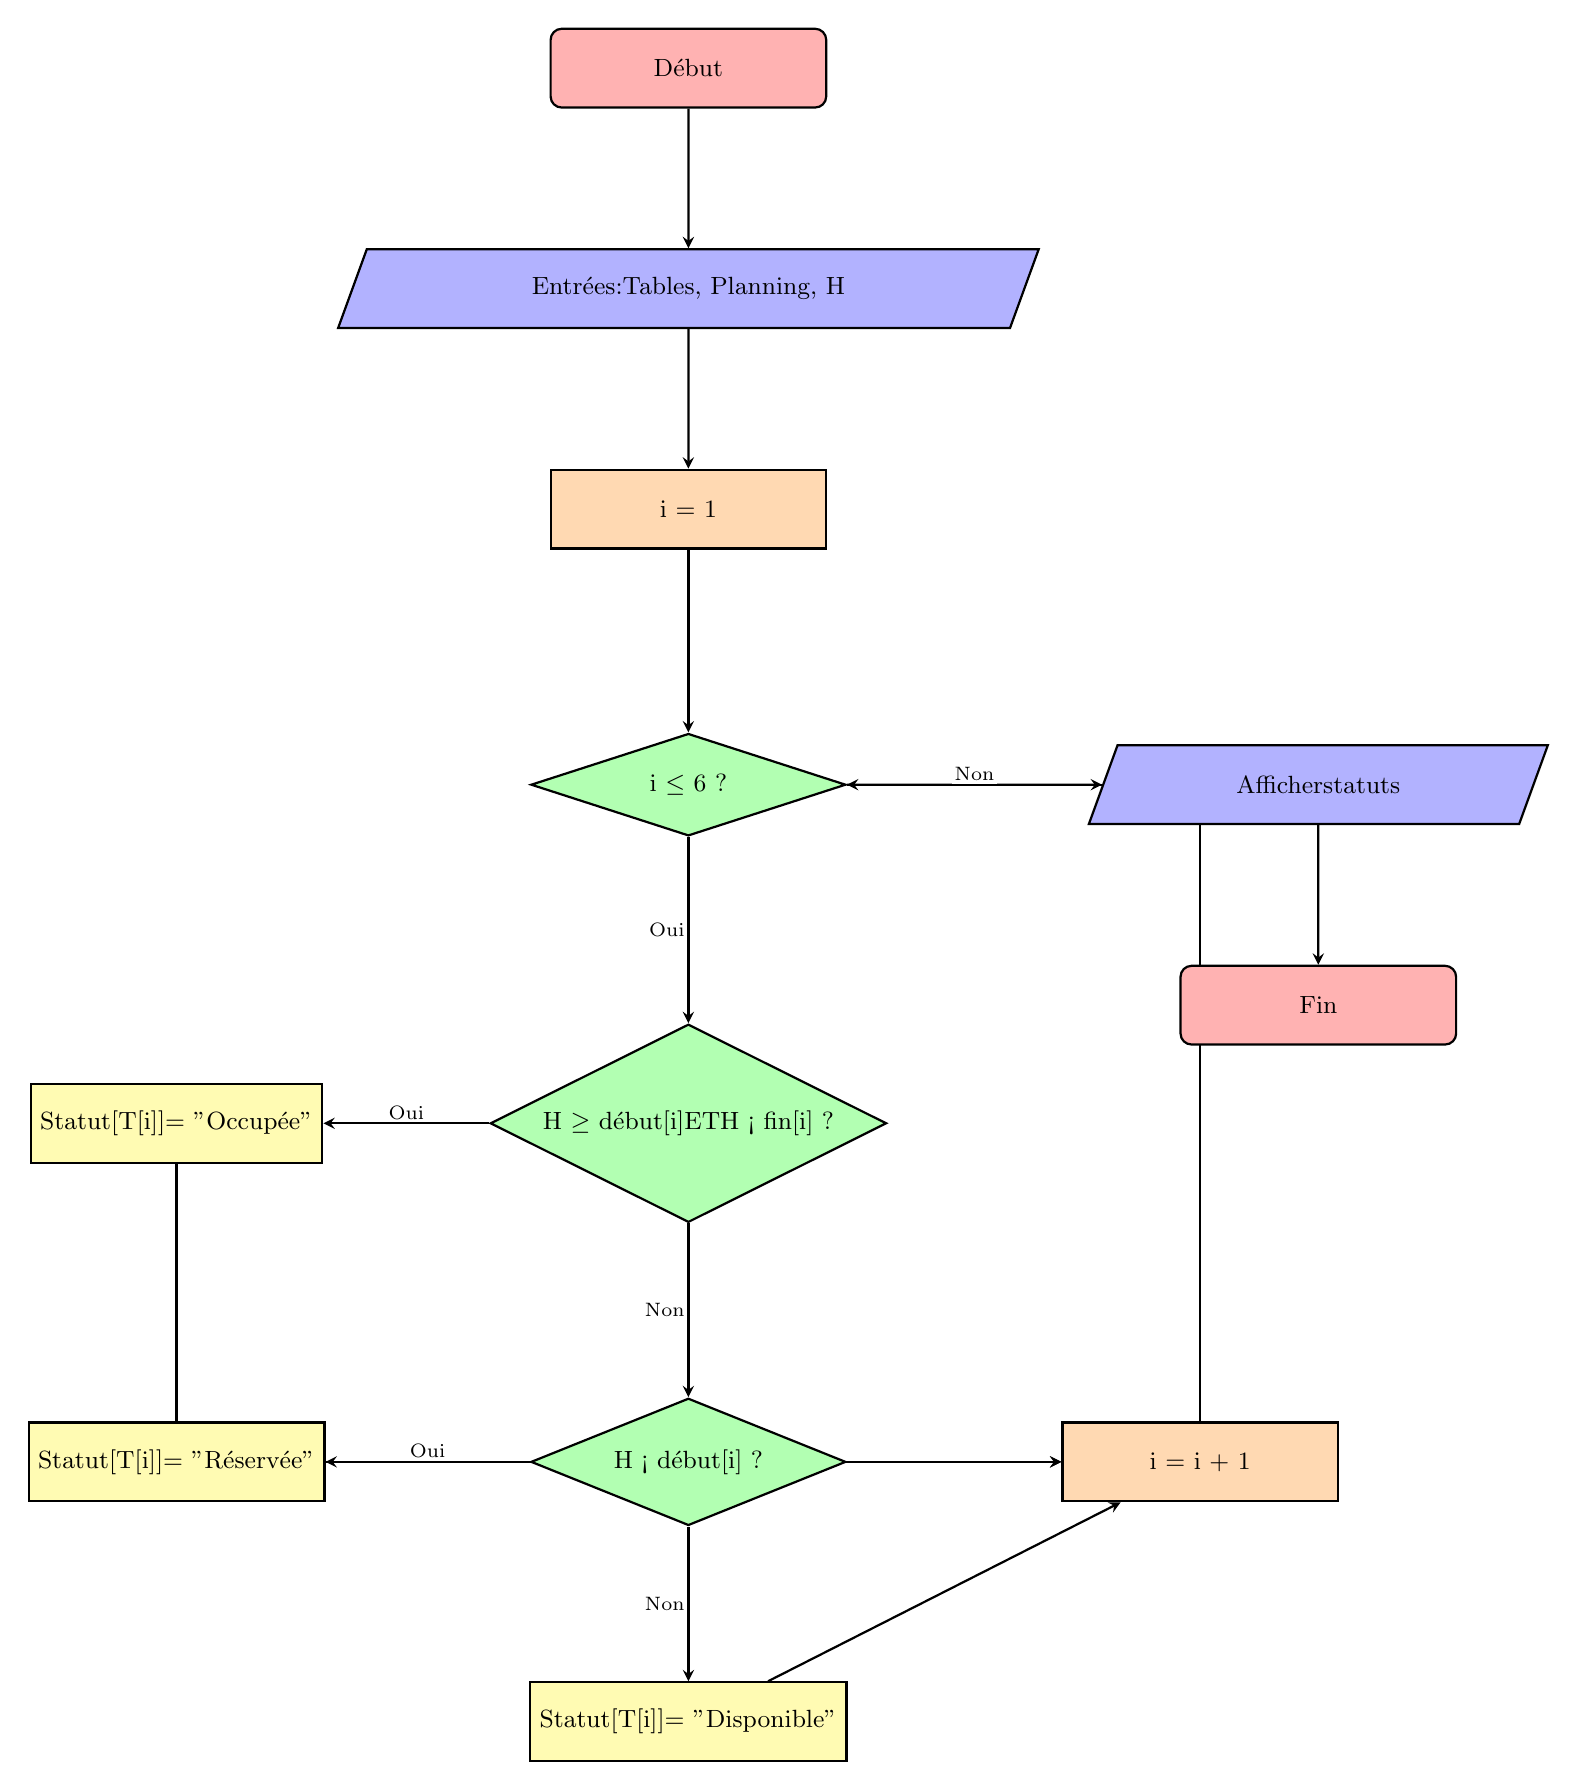
\begin{tikzpicture}[
    node distance=2.5cm,
    startstop/.style={rectangle, rounded corners, minimum width=3.5cm, minimum height=1cm, text centered, draw=black, line width=0.8pt, fill=red!30, font=\small},
    io/.style={trapezium, trapezium left angle=70, trapezium right angle=110, minimum width=3.5cm, minimum height=1cm, text centered, draw=black, line width=0.8pt, fill=blue!30, font=\small},
    process/.style={rectangle, minimum width=3.5cm, minimum height=1cm, text centered, draw=black, line width=0.8pt, fill=orange!30, font=\small},
    decision/.style={diamond, minimum width=4cm, minimum height=1.3cm, text centered, draw=black, line width=0.8pt, fill=green!30, aspect=2, font=\small},
    output/.style={rectangle, minimum width=3.5cm, minimum height=1cm, text centered, draw=black, line width=0.8pt, fill=yellow!30, font=\small},
    arrow/.style={thick,->,>=stealth}
]

% Nodes
\node (start) [startstop] {Début};
\node (input) [io, below of=start, yshift=-0.3cm] {Entrées:\\Tables, Planning, H};
\node (init) [process, below of=input, yshift=-0.3cm] {i = 1};
\node (check) [decision, below of=init, yshift=-1cm] {i $\leq$ 6 ?};
\node (cond1) [decision, below of=check, yshift=-1.8cm] {H $\geq$ début[i]\\ET\\H < fin[i] ?};
\node (status1) [output, left of=cond1, xshift=-4cm] {Statut[T[i]]\\= "Occupée"};
\node (cond2) [decision, below of=cond1, yshift=-1.8cm] {H < début[i] ?};
\node (status2) [output, left of=cond2, xshift=-4cm] {Statut[T[i]]\\= "Réservée"};
\node (status3) [output, below of=cond2, yshift=-0.8cm] {Statut[T[i]]\\= "Disponible"};
\node (increment) [process, right of=cond2, xshift=4cm] {i = i + 1};
\node (display) [io, right of=check, xshift=5.5cm] {Afficher\\statuts};
\node (stop) [startstop, below of=display, yshift=-0.3cm] {Fin};

% Arrows (avec fill=white pour masquer les lignes sous les nœuds)
\begin{scope}[on background layer]
\draw [arrow] (start) -- (input);
\draw [arrow] (input) -- (init);
\draw [arrow] (init) -- (check);
\draw [arrow] (check) -- node[anchor=east, fill=white, inner sep=1pt, font=\scriptsize] {Oui} (cond1);
\draw [arrow] (check) -- node[anchor=south, fill=white, inner sep=1pt, font=\scriptsize] {Non} (display);
\draw [arrow] (cond1) -- node[anchor=south, fill=white, inner sep=1pt, font=\scriptsize] {Oui} (status1);
\draw [arrow] (cond1) -- node[anchor=east, fill=white, inner sep=1pt, font=\scriptsize] {Non} (cond2);
\draw [arrow] (cond2) -- node[anchor=south, fill=white, inner sep=1pt, font=\scriptsize] {Oui} (status2);
\draw [arrow] (cond2) -- node[anchor=east, fill=white, inner sep=1pt, font=\scriptsize] {Non} (status3);
\draw [arrow] (status1) |- (increment);
\draw [arrow] (status2) |- (increment);
\draw [arrow] (status3) -- (increment);
\draw [arrow] (increment) |- (check);
\draw [arrow] (display) -- (stop);
\end{scope}

\end{tikzpicture}%
}
\caption{Diagramme de flux de l'algorithme de gestion des tables de matelassage}
\label{fig:algo_flowchart}
\end{figure}

\subsubsection{Application pratique}
L'algorithme peut etre déployé sous plusieurs formes :
\begin{itemize}
  \item \textbf{Une feuille Excel automatisée}, avec macros et mise a jour minute par minute ;
  \item \textbf{Une interface web locale}, connectée aux données de production et accessible depuis le poste du chef d'atelier.
\end{itemize}

Ce système permet :
\begin{itemize}
  \item De \textbf{visualiser en temps réel} la disponibilité de chaque table ;
  \item D'\textbf{éviter les conflits} ou chevauchements de planning ;
  \item D'\textbf{améliorer la fluidité} du flux de travail entre préparation, matelassage et coupe.
\end{itemize}

\begin{table}[H]
\centering
\caption{Exemple de statut temps réel}
\begin{adjustbox}{max width=\textwidth}
\begin{tabular}{|l|l|l|}
\hline
\textbf{Table} & \textbf{Heure actuelle} & \textbf{Statut} \\
\hline
T1 & 09:00 & Occupée (jusqu'a 09:30) \\
\hline
T2 & 09:00 & Disponible \\
\hline
T3 & 09:00 & Occupée (jusqu'a 09:45) \\
\hline
\end{tabular}
\end{adjustbox}
\end{table}

\subsubsection{Bénéfices attendus}
L'intégration de cet algorithme dans le système de gestion de production offre plusieurs avantages :
\begin{itemize}
  \item \textbf{Réduction du temps d'attente} entre les opérations de coupe ;
  \item \textbf{Optimisation de l'utilisation des ressources existantes} sans investissement matériel supplémentaire ;
  \item \textbf{Amélioration de la coordination} entre opérateurs et planificateurs ;
  \item \textbf{Digitalisation partielle du pilotage de production}, contribuant a la transition vers une \textbf{usine connectée}.
\end{itemize}

Ainsi, cette solution constitue une première étape vers la \textbf{transformation numérique} de l'atelier, en s'inscrivant dans une démarche \textit{Lean 4.0} conciliant \textbf{amélioration continue} et \textbf{technologies intelligentes}.


\subsection{Phase Contrôler : Pérennisation des améliorations}

\subsubsection{Objectifs de la phase de contrôle}

La phase \textbf{Contrôler} (Control) constitue la dernière étape de la méthodologie DMAIC. Elle vise a \textbf{pérenniser les améliorations} mises en place lors de la phase précédente, a \textbf{surveiller les performances} dans le temps, et a garantir que les gains obtenus ne se dégradent pas. Cette phase assure la \textbf{standardisation des nouvelles pratiques} et l'instauration d'un système de \textbf{suivi continu} permettant de détecter rapidement toute dérive.

Dans le contexte de l'atelier de coupe, la phase de contrôle permet de :
\begin{itemize}
  \item Maintenir l'efficacité de l'algorithme de gestion des tables de matelassage ;
  \item Assurer la fiabilité et la mise a jour régulière des données de planification ;
  \item Garantir l'adhésion du personnel aux nouvelles procédures digitales ;
  \item Mettre en place des indicateurs de performance (KPI) pour un pilotage objectif.
\end{itemize}

\subsubsection{Mise en place d'indicateurs de performance (KPI)}

Pour assurer un suivi efficace des améliorations, plusieurs \textbf{indicateurs clés de performance} sont définis et suivis régulièrement :

\begin{table}[H]
\centering
\caption{Indicateurs de performance pour le suivi de l'amélioration}
\small
\renewcommand{\arraystretch}{1.3}
\begin{adjustbox}{max width=\textwidth}
\begin{tabular}{|>{\raggedright\arraybackslash}p{4.5cm}|>{\raggedright\arraybackslash}p{6.5cm}|>{\centering\arraybackslash}p{2cm}|}
\hline
\rowcolor{lightgray}
\textbf{Indicateur} & \textbf{Description} & \textbf{Cible} \\
\hline
Taux de disponibilité des tables & Pourcentage de temps ou les tables sont disponibles sans conflit & > 85\% \\
\hline
Temps d'attente moyen & Temps moyen d'attente entre matelassage et coupe & < 15 min \\
\hline
Nombre de conflits de planning & Nombre de chevauchements ou conflits détectés par semaine & < 3 \\
\hline
Taux d'utilisation de l'algorithme & Fréquence d'utilisation de l'outil de gestion par les opérateurs & > 90\% \\
\hline
Respect du planning & Pourcentage d'opérations réalisées dans les délais prévus & > 80\% \\
\hline
\end{tabular}
\end{adjustbox}
\end{table}

Ces indicateurs sont mesurés de manière \textbf{hebdomadaire} et font l'objet d'une revue mensuelle avec l'équipe de production pour identifier les éventuelles dérives et mettre en place des actions correctives.

\subsubsection{Système de suivi et de visualisation}

Un \textbf{tableau de bord de suivi} est mis en place pour visualiser en temps réel l'évolution des indicateurs de performance. Ce tableau de bord peut prendre la forme :
\begin{itemize}
  \item D'un \textbf{fichier Excel partagé} avec graphiques automatisés (courbes d'évolution, histogrammes) ;
  \item D'un \textbf{dashboard web} accessible depuis les postes de l'atelier, affichant les KPI en temps réel ;
  \item D'un \textbf{affichage visuel} dans l'atelier (écran de supervision) permettant a tous les opérateurs de suivre les performances.
\end{itemize}

\begin{figure}[H]
\centering
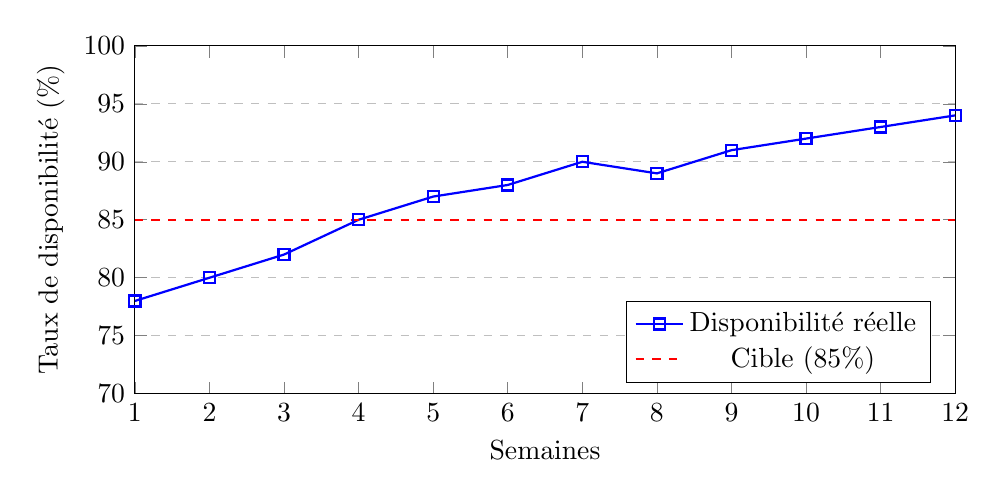
\begin{tikzpicture}
\begin{axis}[
    width=12cm,
    height=6cm,
    xlabel={Semaines},
    ylabel={Taux de disponibilité (\%)},
    ymin=70, ymax=100,
    xmin=1, xmax=12,
    xtick={1,2,3,4,5,6,7,8,9,10,11,12},
    ytick={70,75,80,85,90,95,100},
    legend pos=south east,
    ymajorgrids=true,
    grid style=dashed,
]

\addplot[
    color=blue,
    mark=square,
    thick
    ]
    coordinates {
    (1,78)(2,80)(3,82)(4,85)(5,87)(6,88)(7,90)(8,89)(9,91)(10,92)(11,93)(12,94)
    };
    \addlegendentry{Disponibilité réelle}

\addplot[
    color=red,
    mark=none,
    dashed,
    thick
    ]
    coordinates {
    (1,85)(12,85)
    };
    \addlegendentry{Cible (85\%)}

\end{axis}
\end{tikzpicture}
\caption{Exemple de suivi du taux de disponibilité des tables sur 12 semaines}
\end{figure}

\subsubsection{Mécanismes de contrôle et d'alerte}

Pour garantir la réactivité face aux dérives, des \textbf{mécanismes d'alerte automatiques} sont intégrés au système :
\begin{itemize}
  \item \textbf{Alerte de conflit} : Notification automatique lorsque deux opérations sont planifiées sur la meme table au meme moment ;
  \item \textbf{Alerte de retard} : Signal envoyé au chef d'atelier si une opération dépasse le temps prévu de plus de 20\% ;
  \item \textbf{Alerte de sous-utilisation} : Notification si une table reste inutilisée pendant plus de 2 heures consécutives en période de production ;
  \item \textbf{Rapport hebdomadaire automatique} : Génération d'un rapport récapitulatif des performances envoyé par email aux responsables.
\end{itemize}

Ces alertes permettent une \textbf{intervention rapide} et évitent l'accumulation de dysfonctionnements.

\subsubsection{Standardisation des procédures}

La pérennisation des améliorations passe par la \textbf{formalisation et la standardisation} des nouvelles pratiques. Cela inclut :
\begin{itemize}
  \item \textbf{Rédaction de procédures opératoires standardisées (SOP)} décrivant l'utilisation de l'algorithme de gestion des tables ;
  \item \textbf{Formation du personnel} a l'utilisation de l'outil et aux nouvelles méthodes de planification ;
  \item \textbf{Documentation des bonnes pratiques} : création d'un guide utilisateur illustré, accessible a tous les opérateurs ;
  \item \textbf{Audits réguliers} : vérification trimestrielle du respect des procédures et de l'utilisation effective de l'outil.
\end{itemize}

\subsubsection{Amélioration continue}

La phase de contrôle ne se limite pas a maintenir les acquis, elle s'inscrit dans une logique d'\textbf{amélioration continue} (Kaizen). Des \textbf{réunions d'amélioration} sont organisées mensuellement avec l'équipe de production pour :
\begin{itemize}
  \item Analyser les résultats des indicateurs de performance ;
  \item Identifier les nouvelles opportunités d'optimisation ;
  \item Recueillir les retours d'expérience des opérateurs ;
  \item Ajuster l'algorithme ou les procédures en fonction des besoins terrain.
\end{itemize}

Un \textbf{cycle PDCA} (Plan-Do-Check-Act) est ainsi instauré pour garantir une dynamique d'amélioration permanente.

\subsubsection{Conclusion de la phase Contrôler}

La phase de contrôle assure la \textbf{pérennité des gains} obtenus grace a l'algorithme de gestion des tables de matelassage. En combinant suivi des indicateurs, mécanismes d'alerte, standardisation des pratiques et amélioration continue, cette phase garantit que les bénéfices de la transformation digitale se maintiennent dans le temps et continuent de s'améliorer.

Cette démarche DMAIC complète, de la définition du problème jusqu'au contrôle des solutions, constitue le socle méthodologique de la transformation Lean 4.0 de l'atelier de coupe, préparant ainsi le terrain pour les développements techniques détaillés dans les chapitres suivants.

\chapter{CRISP-ML(Q) phases }\label{chap3:crispml}

\lhead{Chapitre III: Methodologie CRISP-ML(Q)}
\dominitoc 
\rhead{\thepage}
\minitoc

\section{Introduction}\label{chap3:intro}

Ce troisieme chapitre expose de maniere detaillee l'application methodologique de la demarche CRISP-ML(Q) (\textit{Cross-Industry Standard Process for Machine Learning Quality}) \cite{studer2021towards} aux trois premieres phases de notre projet de recherche consacre a l'optimisation de la planification de l'atelier de coupe textile. Cette methodologie structuree, specifiquement adaptee aux exigences et aux specificites du machine learning moderne, integre de maniere systemique les aspects fondamentaux de qualite, de tracabilite et de deploiement continu, essentiels pour garantir la fiabilite et la perennite d'un systeme de production industrielle en environnement operationnel \cite{wirth2000crisp, provost2013data}.

Les phases abordees dans ce chapitre sont :
\begin{itemize}
    \item \textbf{Phase 1 : Comprehension metier (Business Understanding)}
    \item \textbf{Phase 2 : Comprehension des donnees (Data Understanding)}
    \item \textbf{Phase 3 : Preparation des donnees (Data Preparation)}
\end{itemize}

Cette approche methodologique garantit une transition fluide vers les phases de modelisation et de deploiement, tout en assurant la qualite et la tracabilite des decisions prises.

\subsection{Vue d'ensemble du processus CRISP-ML(Q)}

La figure \ref{fig:crispml_process} illustre le processus complet CRISP-ML(Q) avec ses 6 phases iteratives et les boucles de retroaction qualite.

\begin{figure}[H]
\centering
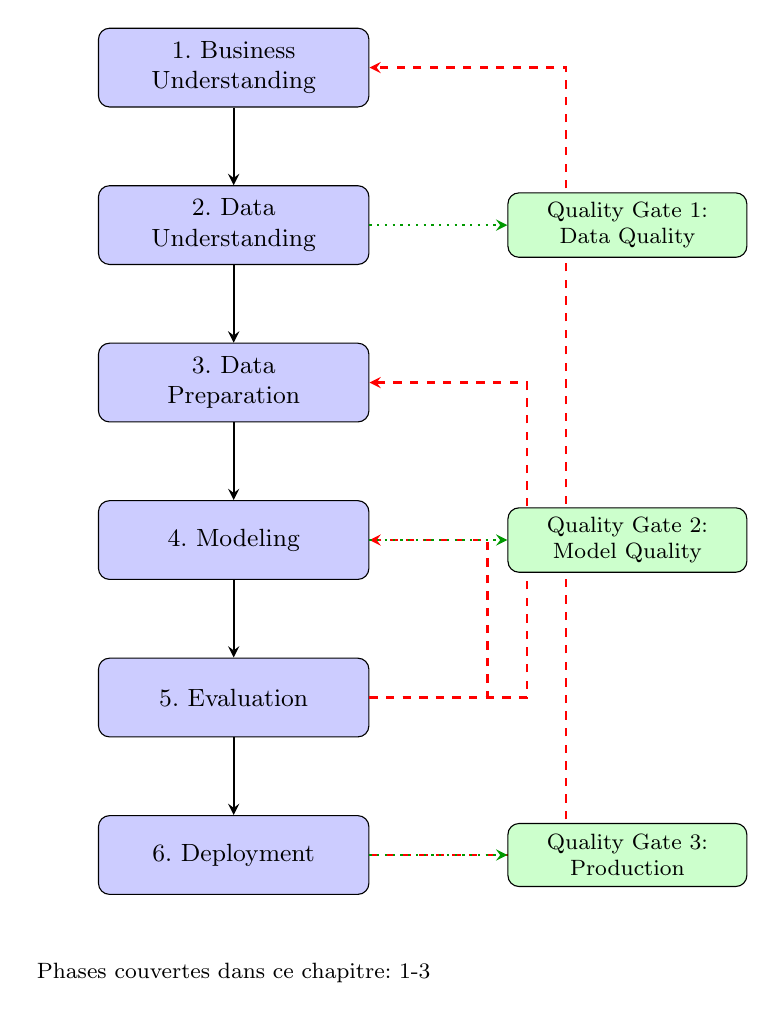
\begin{tikzpicture}[
    node distance=1.8cm,
    phase/.style={rectangle, draw, fill=blue!20, text width=3.2cm, text centered, rounded corners, minimum height=1cm, font=\small},
    arrow/.style={->, >=stealth, thick},
    quality/.style={rectangle, draw, fill=green!20, text width=2.8cm, text centered, rounded corners, minimum height=0.8cm, font=\footnotesize}
]

% Phases principales (colonne gauche)
\node[phase] (business) at (0,0) {1. Business\\Understanding};
\node[phase] (data) at (0,-2) {2. Data\\Understanding};
\node[phase] (prep) at (0,-4) {3. Data\\Preparation};
\node[phase] (model) at (0,-6) {4. Modeling};
\node[phase] (eval) at (0,-8) {5. Evaluation};
\node[phase] (deploy) at (0,-10) {6. Deployment};

% Fleches principales
\draw[arrow] (business) -- (data);
\draw[arrow] (data) -- (prep);
\draw[arrow] (prep) -- (model);
\draw[arrow] (model) -- (eval);
\draw[arrow] (eval) -- (deploy);

% Boucles de retroaction (a droite)
\draw[arrow, dashed, red] (eval.east) -- ++(1.5,0) |- (model.east);
\draw[arrow, dashed, red] (eval.east) -- ++(2,0) |- (prep.east);
\draw[arrow, dashed, red] (deploy.east) -- ++(2.5,0) |- (business.east);

% Quality gates (colonne droite)
\node[quality] (qg1) at (5,-2) {Quality Gate 1:\\Data Quality};
\node[quality] (qg2) at (5,-6) {Quality Gate 2:\\Model Quality};
\node[quality] (qg3) at (5,-10) {Quality Gate 3:\\Production};

\draw[arrow, dotted, green!60!black] (data.east) -- (qg1.west);
\draw[arrow, dotted, green!60!black] (model.east) -- (qg2.west);
\draw[arrow, dotted, green!60!black] (deploy.east) -- (qg3.west);

% Legende
\node[font=\footnotesize] at (0,-11.5) {Phases couvertes dans ce chapitre: 1-3};

\end{tikzpicture}
\caption{Processus CRISP-ML(Q) avec portes de qualite}
\label{fig:crispml_process}
\end{figure}

\textbf{Caracteristiques cles du processus :}
\begin{itemize}
    \item \textbf{Iteratif} : Retours possibles vers les phases precedentes
    \item \textbf{Qualite integree} : Portes de qualite a chaque etape critique
    \item \textbf{Tracabilite} : Documentation complete des decisions
    \item \textbf{Reproductibilite} : Processus standardise et automatise
\end{itemize}

\section{Outils et bibliothèques utilisés}\label{chap3:tools}

\subsection{Introduction}

Le choix des outils et des bibliothèques constitue une décision stratégique fondamentale dans tout projet de machine learning industriel. Ces choix technologiques influencent directement la qualité, la performance, la maintenabilité et la pérennité de la solution développée. Dans le contexte de ce projet d'optimisation de la planification de l'atelier de coupe textile, la sélection des technologies s'est appuyée sur des critères rigoureux et objectifs, alignés avec les exigences de la méthodologie CRISP-ML(Q) et les contraintes opérationnelles de l'environnement industriel.

Les critères de sélection appliqués incluent : (1) la \textbf{maturité technologique} et la stabilité des bibliothèques, garantissant une fiabilité en production ; (2) la \textbf{performance} mesurée par des benchmarks objectifs ; (3) la \textbf{qualité de la documentation} et l'activité de la communauté, facilitant le développement et la maintenance ; (4) la \textbf{compatibilité} et l'interopérabilité entre les différents composants de la stack ; et (5) la \textbf{maintenabilité} à long terme, essentielle pour l'évolution du système.

Cette section présente de manière structurée l'écosystème technologique complet du projet, organisé en cinq catégories principales : l'écosystème Data Science et Machine Learning, les frameworks de développement backend et frontend, les outils d'optimisation et d'ordonnancement, l'infrastructure DevOps, et enfin une synthèse de la stack technologique complète avec son intégration dans la méthodologie CRISP-ML(Q).

\subsection{Écosystème Data Science et Machine Learning}

L'écosystème Data Science constitue le cœur technique du projet, regroupant les bibliothèques essentielles pour la manipulation des données, l'entraînement des modèles et la visualisation des résultats. L'ensemble de cet écosystème est développé en \textbf{Python 3.11.0}, langage de programmation de référence pour le Data Science et le Machine Learning, offrant une syntaxe claire, une vaste collection de bibliothèques scientifiques et une communauté active.
\begin{figure}[H]
\centering
\includegraphics[width=0.7\textwidth]{Chapitre3/images/python.png}
\caption{Langage de programmation Python}
\label{fig:3.2}
\end{figure}

\subsubsection{Bibliothèques de manipulation de données}


\begin{table}[H]
\centering
\caption{Bibliothèques Python pour la manipulation de données}
\begin{tabular}{|l|l|p{3cm}|p{6cm}|}
\hline
\textbf{Bibliothèque} & \textbf{Version} & \textbf{Rôle principal} & \textbf{Justification du choix} \\
\hline
\textbf{pandas} & 2.0.3 & Manipulation et analyse de données tabulaires & Standard de l'industrie pour les DataFrames, API riche et intuitive, performance optimisée pour les opérations vectorisées, intégration native avec NumPy et scikit-learn \\
\hline
\textbf{NumPy} & 1.24.3 & Calculs numériques et algèbre linéaire & Fondation de l'écosystème scientifique Python, performance optimale pour les opérations matricielles, support natif des types numériques, base de toutes les bibliothèques ML \\
\hline
\end{tabular}
\label{tab:data_manipulation_libs}
\end{table}

\textbf{pandas} est utilisé intensivement dans les phases Data Understanding et Data Preparation de CRISP-ML(Q) pour le chargement, le nettoyage, la transformation et l'analyse exploratoire du dataset principal (\texttt{PSC\_X\_1 - COUPE.csv}, 16,433 enregistrements). Ses fonctionnalités de groupement, d'agrégation et de manipulation temporelle sont essentielles pour l'ingénierie des caractéristiques.

\textbf{NumPy} fournit les structures de données fondamentales (arrays multidimensionnels) et les opérations mathématiques de bas niveau utilisées par toutes les autres bibliothèques. Son utilisation garantit des performances optimales pour les calculs vectorisés et matriciels nécessaires au preprocessing et aux transformations de données.

\begin{figure}[H]
\centering
\includegraphics[width=0.8\textwidth]{Chapitre3/images/pbib.png}
\caption{Bibliothèques de manipulation de données - pandas et NumPy}
\label{fig:bib_manipulation}
\end{figure}

\subsubsection{Bibliothèques de Machine Learning}

\begin{table}[H]
\centering
\caption{Bibliothèques Python pour le Machine Learning}
\begin{tabular}{|l|l|p{3cm}|p{6cm}|}
\hline
\textbf{Bibliothèque} & \textbf{Version} & \textbf{Rôle principal} & \textbf{Justification du choix} \\
\hline
\textbf{scikit-learn} & 1.3.0 & Preprocessing, métriques, validation croisée & API cohérente et standardisée, documentation exhaustive, implémentation robuste des algorithmes classiques, outils de validation et d'évaluation complets \\
\hline
\textbf{XGBoost} & 1.7.6 & Algorithme principal de prédiction des temps & Performance supérieure (R²=0.84, MAE=12.3 min), gestion native des valeurs manquantes, régularisation intégrée (L1/L2), interprétabilité via SHAP, temps d'entraînement optimal (< 1 min) \\
\hline
\end{tabular}
\label{tab:ml_libs}
\end{table}

\textbf{scikit-learn} est utilisé pour le preprocessing des données (\texttt{StandardScaler}, \texttt{LabelEncoder}), la séparation train/test (\texttt{train\_test\_split}), la validation croisée temporelle, et le calcul des métriques de performance (R², MAE, RMSE, MAPE). Son API uniforme facilite l'expérimentation avec différents algorithmes.

\textbf{XGBoost} (Extreme Gradient Boosting) \cite{chen2016xgboost} a été sélectionné comme algorithme principal après une comparaison rigoureuse avec six alternatives (Régression Linéaire, Ridge, Lasso, Random Forest, Gradient Boosting). Les résultats expérimentaux démontrent sa supériorité statistiquement significative (test de Wilcoxon, p=0.031) avec un R² de 0.84 contre 0.78 pour Random Forest, représentant une amélioration de +87\% par rapport à la régression linéaire. Ses avantages incluent la régularisation intégrée prévenant le surapprentissage, la gestion native des valeurs manquantes, la parallélisation efficace, et l'interprétabilité via les valeurs SHAP. Le temps d'entraînement de 45 secondes offre un excellent compromis performance/rapidité pour le réentraînement périodique.

\textbf{Alternatives considérées :}
\begin{itemize}
    \item \textbf{Random Forest} : Performance inférieure (R²=0.78) et temps d'entraînement plus long (12.5 min)
    \item \textbf{Gradient Boosting} : Performance légèrement inférieure (R²=0.81) et temps d'entraînement excessif (78.2 min)
    \item \textbf{Régression linéaire} : Performance insuffisante (R²=0.45) pour les besoins du projet
\end{itemize}

\begin{figure}[H]
\centering
\includegraphics[width=0.7\textwidth]{Chapitre3/images/python.png}
\caption{Logo Python - Langage de programmation utilisé pour l'écosystème Machine Learning (Python 3.11.0)}
\label{fig:python_logo}
\end{figure}

\subsubsection{Bibliothèques de visualisation}

\begin{table}[H]
\centering
\caption{Bibliothèques Python pour la visualisation}
\begin{tabular}{|l|l|p{3cm}|p{6cm}|}
\hline
\textbf{Bibliothèque} & \textbf{Version} & \textbf{Rôle principal} & \textbf{Justification du choix} \\
\hline
\textbf{matplotlib} & 3.7.2 & Visualisations statiques de base & Bibliothèque de référence pour les graphiques scientifiques, contrôle fin de tous les éléments visuels, export haute qualité pour publications \\
\hline
\textbf{seaborn} & 0.12.2 & Visualisations statistiques avancées & Intégration native avec pandas, esthétique professionnelle par défaut, fonctions statistiques intégrées (distributions, corrélations, régression) \\
\hline
\end{tabular}
\label{tab:viz_libs}
\end{table}

Ces bibliothèques sont utilisées intensivement dans la phase Data Understanding pour l'analyse exploratoire des données (EDA) : distributions des variables, matrices de corrélation, détection des outliers, analyse des patterns temporels, et visualisation des performances des modèles (courbes d'apprentissage, importance des features, résidus).

\begin{figure}[H]
\centering
\IfFileExists{Chapitre3/images/logos/figure-28-data-science.png}{%
    \includegraphics[width=0.9\textwidth]{Chapitre3/images/logos/figure-28-data-science.png}
}{%
    \fbox{\parbox{0.9\textwidth}{\centering\vspace{3cm}Figure 28 - Écosystème Data Science\\(pandas, NumPy, scikit-learn, XGBoost, matplotlib, seaborn)\\\vspace{3cm}}}
}
\caption{Écosystème Data Science et Machine Learning utilisé dans le projet (pandas 2.0.3, NumPy 1.24.3, scikit-learn 1.3.0, XGBoost 1.7.6, matplotlib 3.7.2, seaborn 0.12.2)}
\label{fig:data_science_logos}
\end{figure}

\subsection{Frameworks de développement}

Les frameworks de développement assurent la création d'une application web complète, robuste et performante, intégrant les modèles ML dans un environnement de production opérationnel.

\subsubsection{Backend et API}

\begin{table}[H]
\centering
\caption{Technologies backend et API}
\begin{tabular}{|l|l|p{3cm}|p{6cm}|}
\hline
\textbf{Technologie} & \textbf{Version} & \textbf{Rôle principal} & \textbf{Justification du choix} \\
\hline
\textbf{FastAPI} & 0.103.0 & Framework web moderne pour API REST & Performance exceptionnelle (async/await natif), documentation automatique (Swagger/OpenAPI), validation de données intégrée (Pydantic), type hints Python natifs, temps de réponse < 200ms \\
\hline
\textbf{Pydantic} & 2.3.0 & Validation et sérialisation de données & Validation automatique des types, génération de schémas JSON, performance optimale, intégration native avec FastAPI \\
\hline
\textbf{uvicorn} & 0.23.2 & Serveur ASGI haute performance & Support async/await, performance optimale, compatibilité ASGI, déploiement production \\
\hline
\end{tabular}
\label{tab:backend_tech}
\end{table}

\textbf{FastAPI} a été choisi comme framework backend principal pour plusieurs raisons techniques et opérationnelles majeures. Premièrement, sa performance exceptionnelle basée sur le support natif de la programmation asynchrone (async/await) permet de gérer efficacement les requêtes concurrentes avec une latence minimale (< 200ms pour les prédictions individuelles, débit de 1000 prédictions/minute). Deuxièmement, la génération automatique de documentation interactive (Swagger UI et ReDoc) facilite l'intégration et le test des endpoints par les développeurs frontend et les utilisateurs. Troisièmement, l'intégration native avec Pydantic assure une validation robuste des données d'entrée et de sortie, réduisant les erreurs et améliorant la fiabilité. Enfin, l'utilisation des type hints Python modernes améliore la maintenabilité du code et permet la détection précoce des erreurs via les outils d'analyse statique.

\textbf{Alternatives considérées :}
\begin{itemize}
    \item \textbf{Flask} : Framework plus simple mais performance inférieure (pas de support async natif), documentation manuelle requise
    \item \textbf{Django} : Framework trop lourd pour une API pure, overhead inutile, temps de réponse plus élevés
\end{itemize}

\begin{figure}[H]
\centering
\IfFileExists{Chapitre3/images/logos/figure-31-backend.png}{%
    \includegraphics[width=0.7\textwidth]{Chapitre3/images/logos/figure-31-backend.png}
}{%
    \fbox{\parbox{0.7\textwidth}{\centering\vspace{2cm}Figure 31 - Technologies Backend\\(FastAPI, Pydantic, uvicorn)\\\vspace{2cm}}}
}
\caption{Technologies backend et serveur ASGI (FastAPI 0.103.0, Pydantic 2.3.0, uvicorn 0.23.2)}
\label{fig:backend_logos}
\end{figure}

\subsubsection{Frontend et interface utilisateur}

\begin{table}[H]
\centering
\caption{Technologies frontend}
\begin{tabular}{|l|l|p{3cm}|p{6cm}|}
\hline
\textbf{Technologie} & \textbf{Version} & \textbf{Rôle principal} & \textbf{Justification du choix} \\
\hline
\textbf{React} & 18.2.0 & Framework JavaScript pour interface utilisateur & Architecture composants réutilisables, Virtual DOM pour performance, écosystème riche, communauté active, support TypeScript \\
\hline
\textbf{Recharts} & 2.8.0 & Bibliothèque de visualisations interactives & Composants React natifs, visualisations responsives, personnalisation facile, performance optimale \\
\hline
\textbf{Axios} & 1.5.0 & Client HTTP pour communication API & API simple et intuitive, intercepteurs pour authentification, gestion des erreurs robuste, support des promesses \\
\hline
\end{tabular}
\label{tab:frontend_tech}
\end{table}

\textbf{React} offre une architecture moderne basée sur des composants réutilisables, facilitant le développement et la maintenance de l'interface utilisateur. Le Virtual DOM assure des performances optimales lors des mises à jour fréquentes du dashboard en temps réel. L'écosystème riche (React Router, Redux, hooks) et la communauté active garantissent la disponibilité de solutions pour tous les besoins. Le support natif de TypeScript améliore la robustesse du code frontend.

\textbf{Recharts} fournit des composants de visualisation interactifs parfaitement intégrés avec React, utilisés pour afficher les KPIs, les graphiques de performance, les plannings visuels et les tableaux de bord opérationnels. Sa nature responsive assure une expérience utilisateur optimale sur tous les appareils.

\begin{figure}[H]
\centering
\IfFileExists{Chapitre3/images/logos/figure-34-frontend.png}{%
    \includegraphics[width=0.7\textwidth]{Chapitre3/images/logos/figure-34-frontend.png}
}{%
    \fbox{\parbox{0.7\textwidth}{\centering\vspace{2cm}Figure 34 - Technologies Frontend\\(React, Recharts, Axios)\\\vspace{2cm}}}
}
\caption{Technologies frontend et communication API (React 18.2.0, Recharts 2.8.0, Axios 1.5.0)}
\label{fig:frontend_logos}
\end{figure}

\subsection{Outils d'optimisation et d'ordonnancement}

L'optimisation de l'ordonnancement des tables de matelassage constitue un composant critique du système, nécessitant des outils spécialisés en recherche opérationnelle.

\begin{table}[H]
\centering
\caption{Outils d'optimisation}
\begin{tabular}{|l|l|p{3cm}|p{6cm}|}
\hline
\textbf{Outil} & \textbf{Version} & \textbf{Rôle principal} & \textbf{Justification du choix} \\
\hline
\textbf{OR-Tools} & 9.7 & Bibliothèque d'optimisation Google & Solveurs performants (CP-SAT, LP, MIP), documentation complète, support contraintes complexes, gratuit et open-source, maintenance active \\
\hline
\textbf{CP-SAT Solver} & 9.7 & Solveur de programmation par contraintes & Performance exceptionnelle pour problèmes d'ordonnancement, support contraintes temporelles, résolution < 2 secondes pour 50 OF, optimisation multi-critères \\
\hline
\end{tabular}
\label{tab:optimization_tools}
\end{table}

\textbf{OR-Tools} de Google est une bibliothèque de recherche opérationnelle de niveau industriel, offrant plusieurs solveurs spécialisés. Le \textbf{CP-SAT Solver} (Constraint Programming - Satisfiability) a été sélectionné pour résoudre le problème d'ordonnancement optimal des tables de matelassage. Ce solveur excelle dans les problèmes combinatoires avec contraintes temporelles complexes (disponibilité des tables, séquencement des opérations, respect des délais, équilibrage de charge).

Les performances mesurées démontrent une résolution en moins de 2 secondes pour un planning de 50 ordres de fabrication, avec optimisation simultanée de trois critères : minimisation du makespan (durée totale), équilibrage de la charge entre les tables, et respect des priorités clients. Cette performance permet une reoptimisation dynamique en cas de perturbation (panne machine, retard), assurant la réactivité du système.

\textbf{Formulation du problème :} Le problème d'ordonnancement est modélisé comme un problème de satisfaction de contraintes avec variables de décision (affectation table-OF, temps de début), contraintes (non-chevauchement, précédence, capacité), et fonction objectif multi-critères. Le solveur CP-SAT explore l'espace des solutions de manière efficace grâce à des techniques de propagation de contraintes et de recherche arborescente.

\subsection{Infrastructure et DevOps}

L'infrastructure et les outils DevOps assurent la reproductibilité, la qualité et le déploiement fiable du système en environnement de production.

\begin{table}[H]
\centering
\caption{Outils d'infrastructure et DevOps}
\begin{tabular}{|l|l|p{3cm}|p{6cm}|}
\hline
\textbf{Outil} & \textbf{Version} & \textbf{Rôle principal} & \textbf{Justification du choix} \\
\hline
\textbf{Docker} & 24.0 & Conteneurisation des applications & Reproductibilité garantie, isolation des dépendances, déploiement simplifié, portabilité multi-environnements \\
\hline
\textbf{Git} & 2.41 & Gestion de version du code source & Standard de l'industrie, collaboration efficace, traçabilité complète, intégration CI/CD \\
\hline
\textbf{pytest} & 7.4.0 & Framework de tests automatisés & Syntaxe simple et expressive, fixtures puissantes, couverture de code, intégration CI/CD \\
\hline
\textbf{PostgreSQL} & 15.3 & Base de données relationnelle & Fiabilité éprouvée, support transactions ACID, performance optimale, types de données riches \\
\hline
\end{tabular}
\label{tab:devops_tools}
\end{table}

\textbf{Docker} assure la conteneurisation de tous les composants du système (API FastAPI, modèles ML, base de données), garantissant une reproductibilité parfaite entre les environnements de développement, test et production. L'isolation des dépendances prévient les conflits de versions et simplifie le déploiement.

\textbf{Git} est utilisé pour la gestion de version du code source, des configurations et de la documentation, assurant une traçabilité complète des modifications et facilitant la collaboration entre les membres de l'équipe.

\textbf{pytest} fournit un framework de tests automatisés couvrant les tests unitaires (fonctions individuelles), les tests d'intégration (interaction entre composants), et les tests end-to-end (scénarios utilisateur complets). La couverture de code cible est de 80\%, assurant la robustesse du système.

\textbf{PostgreSQL} est utilisé comme base de données relationnelle pour la persistance des données de production (ordres de fabrication, historique des prédictions, logs système, configurations). Son support des transactions ACID garantit la cohérence des données, et ses performances sont optimales pour les requêtes analytiques.

\begin{figure}[H]
\centering
\IfFileExists{Chapitre3/images/logos/figure-35-devops.png}{%
    \includegraphics[width=0.9\textwidth]{Chapitre3/images/logos/figure-35-devops.png}
}{%
    \fbox{\parbox{0.9\textwidth}{\centering\vspace{3cm}Figure 35 - Infrastructure DevOps\\(Docker, Git, pytest, PostgreSQL, OR-Tools)\\\vspace{3cm}}}
}
\caption{Infrastructure DevOps et outils de déploiement (Docker 24.0, Git 2.41, pytest 7.4.0, PostgreSQL 15.3, OR-Tools 9.7)}
\label{fig:devops_logos}
\end{figure}

\subsection{Stack technologique complète}

Le tableau suivant présente une vue d'ensemble synthétique de la stack technologique complète, organisée par couche fonctionnelle.

\begin{table}[H]
\centering
\caption{Stack technologique complète du projet}
\begin{tabular}{|l|p{5cm}|p{6cm}|}
\hline
\textbf{Couche} & \textbf{Technologies} & \textbf{Rôle dans le système} \\
\hline
\textbf{Data Science \& ML} & pandas 2.0.3, NumPy 1.24.3, scikit-learn 1.3.0, XGBoost 1.7.6, matplotlib 3.7.2, seaborn 0.12.2 & Manipulation de données, entraînement des modèles ML, analyse exploratoire, visualisation des résultats, évaluation des performances \\
\hline
\textbf{Backend \& API} & FastAPI 0.103.0, Pydantic 2.3.0, uvicorn 0.23.2 & API REST haute performance, validation de données, endpoints de prédiction et d'ordonnancement, authentification \\
\hline
\textbf{Frontend} & React 18.2.0, Recharts 2.8.0, Axios 1.5.0 & Interface utilisateur responsive, dashboard interactif, visualisations temps réel, communication avec l'API \\
\hline
\textbf{Optimisation} & OR-Tools 9.7, CP-SAT Solver 9.7 & Ordonnancement optimal des tables, résolution de contraintes, optimisation multi-critères \\
\hline
\textbf{Base de données} & PostgreSQL 15.3, SQLAlchemy 2.0.20 & Persistance des données, historique des prédictions, logs système, gestion des configurations \\
\hline
\textbf{DevOps \& Infrastructure} & Docker 24.0, Git 2.41, pytest 7.4.0 & Conteneurisation, gestion de version, tests automatisés, déploiement continu \\
\hline
\end{tabular}
\label{tab:complete_stack}
\end{table}

Cette stack technologique a été conçue pour assurer une intégration harmonieuse entre tous les composants, de la collecte des données jusqu'au déploiement en production. Chaque technologie a été sélectionnée pour sa maturité, sa performance et sa compatibilité avec les autres composants, garantissant ainsi la fiabilité et la maintenabilité à long terme du système.

\subsection{Justification des choix et intégration CRISP-ML(Q)}

Les choix technologiques effectués s'alignent rigoureusement avec les six phases de la méthodologie CRISP-ML(Q), assurant une couverture complète du cycle de vie du projet de machine learning.

\textbf{Alignement avec les phases CRISP-ML(Q) :}

\begin{itemize}
    \item \textbf{Phase 1 - Business Understanding} : Git pour la documentation et la traçabilité des décisions, outils de collaboration pour l'alignement avec les parties prenantes
    
    \item \textbf{Phase 2 - Data Understanding} : pandas pour l'exploration des données (16,433 enregistrements), matplotlib et seaborn pour l'analyse exploratoire (distributions, corrélations, outliers), NumPy pour les calculs statistiques
    
    \item \textbf{Phase 3 - Data Preparation} : pandas pour le nettoyage et la transformation, scikit-learn pour le preprocessing (StandardScaler, encodage), gestion des valeurs manquantes et des outliers
    
    \item \textbf{Phase 4 - Modeling} : XGBoost pour l'entraînement du modèle principal, scikit-learn pour la validation croisée temporelle, OR-Tools CP-SAT pour l'optimisation de l'ordonnancement
    
    \item \textbf{Phase 5 - Evaluation} : scikit-learn pour les métriques (R², MAE, RMSE, MAPE), matplotlib pour les courbes d'apprentissage et l'analyse des résidus, tests statistiques de significativité
    
    \item \textbf{Phase 6 - Deployment} : FastAPI pour l'API de production, Docker pour la conteneurisation, PostgreSQL pour la persistance, React pour l'interface utilisateur, pytest pour les tests automatisés
\end{itemize}

\textbf{Critères de sélection appliqués :}

\begin{enumerate}
    \item \textbf{Maturité technologique} : Toutes les bibliothèques sélectionnées sont des standards de l'industrie avec un historique stable (pandas depuis 2008, scikit-learn depuis 2007, XGBoost depuis 2014, FastAPI depuis 2018 avec adoption rapide)
    
    \item \textbf{Performance mesurée} : Les choix sont justifiés par des benchmarks objectifs (XGBoost R²=0.84 vs alternatives, FastAPI latence < 200ms, CP-SAT résolution < 2s)
    
    \item \textbf{Qualité de la documentation} : Toutes les technologies disposent d'une documentation exhaustive, de tutoriels complets et d'une communauté active (Stack Overflow, GitHub, forums spécialisés)
    
    \item \textbf{Compatibilité et interopérabilité} : L'écosystème Python assure une intégration harmonieuse entre les composants Data Science, l'API FastAPI expose les modèles de manière standard (REST/JSON), React communique via HTTP standard
    
    \item \textbf{Maintenabilité à long terme} : Le code est structuré selon les bonnes pratiques (type hints, tests automatisés, documentation inline), les dépendances sont gérées via requirements.txt, Docker assure la reproductibilité
\end{enumerate}

\textbf{Bénéfices de la stack choisie :}

\begin{itemize}
    \item \textbf{Reproductibilité scientifique} : Docker et Git garantissent que les résultats peuvent être reproduits exactement, essentiel pour la validation académique et industrielle
    
    \item \textbf{Performance opérationnelle} : La stack optimisée (XGBoost, FastAPI async, CP-SAT) assure des temps de réponse compatibles avec les contraintes temps réel de la production (< 2 secondes)
    
    \item \textbf{Maintenabilité à long terme} : L'utilisation de standards de l'industrie, la documentation complète et les tests automatisés facilitent l'évolution et la maintenance du système
    
    \item \textbf{Évolutivité du système} : L'architecture modulaire (API REST, microservices potentiels) permet d'ajouter de nouvelles fonctionnalités sans refonte majeure
\end{itemize}

Cette stack technologique constitue ainsi un fondement solide pour le développement, le déploiement et la maintenance d'un système d'intelligence artificielle industriel performant, fiable et évolutif, répondant aux exigences rigoureuses de la méthodologie CRISP-ML(Q) et aux contraintes opérationnelles de l'environnement de production textile.

\section{Phase 1 : Comprehension metier (Business Understanding)}\label{chap3:business}

\subsection{Contexte strategique et enjeux}

La phase de comprehension metier etablit les fondations du projet de machine learning en alignant les objectifs techniques avec les besoins strategiques de l'entreprise. Cette phase critique garantit que la solution developpee apportera une valeur metier mesurable et durable.

\subsubsection{Contexte industriel}

L'industrie textile tunisienne fait face a une concurrence internationale accrue et a des exigences croissantes en termes de delais et de qualite. BACOVET, acteur majeur du secteur, doit moderniser ses processus pour maintenir sa competitivite. L'atelier de coupe, maillon critique de la chaine de production, represente un goulot d'etranglement potentiel dont l'optimisation peut generer des gains significatifs.

\textbf{Enjeux strategiques :}
\begin{itemize}
    \item \textbf{Competitivite} : Reduire les coûts de production de 8\% via l'optimisation
    \item \textbf{Qualite de service} : Ameliorer le taux de respect des delais de 85\% a 95\%
    \item \textbf{Transformation digitale} : Positionner BACOVET comme leader de l'Industrie 4.0 dans le textile
    \item \textbf{Capitalisation des connaissances} : Reduire la dependance aux experts individuels
    \item \textbf{Scalabilite} : Creer un modele reproductible pour d'autres ateliers
\end{itemize}

\subsection{Business Model Canvas}

Le Business Model Canvas permet de visualiser la proposition de valeur du systeme IA dans l'ecosysteme de l'entreprise.

\begin{table}[H]
\centering
\caption{Business Model Canvas du systeme IA de planification}
\begin{tabular}{|l|l|}
\hline
\multicolumn{2}{|c|}{\textbf{Proposition de valeur}} \\
\hline
\multicolumn{2}{|l|}{Systeme intelligent de planification optimisant l'utilisation des ressources, reduisant les delais et ameliorant la precision des estimations grâce a l'IA} \\
\hline
\textbf{Segments clients} & \textbf{Relations clients} \\
\hline
- Chefs d'atelier (planification) & - Support dedie \\
- Planificateurs (optimisation) & - Formation continue \\
- Operateurs (execution) & - Feedback regulier \\
- Direction (pilotage) & - Comite de pilotage \\
\hline
\textbf{Canaux} & \textbf{Flux de revenus} \\
\hline
- Application web responsive & - Gains productivite : 18,000 TND/an \\
- Dashboard temps reel & - Reduction retards : 8,000 TND/an \\
- Notifications push/email & - Optimisation capacite : 28,000 TND/an \\
- API pour integrations & - Reduction HS : 12,000 TND/an \\
\hline
\textbf{Activites cles} & \textbf{Ressources cles} \\
\hline
- Prediction temps ML & - Donnees historiques (16K+ records) \\
- Optimisation ordonnancement & - Modeles ML (XGBoost, CP-SAT) \\
- Monitoring temps reel & - Infrastructure cloud \\
- Amelioration continue & - Équipe data science \\
\hline
\textbf{Partenaires cles} & \textbf{Structure de coûts} \\
\hline
- Fournisseur G.Pro (ERP) & - Developpement : 35,000 TND \\
- Fournisseur Divatex (CAO) & - Infrastructure : 15,000 TND \\
- Prestataire cloud & - Formation : 7,500 TND \\
- Experts ML externes & - Support : 5,000 TND/an \\
\hline
\end{tabular}
\label{tab:business_model_canvas}
\end{table}

\subsection{Objectifs metier detailles}

L'objectif principal du projet est de developper un systeme d'intelligence artificielle pour optimiser la planification de l'atelier de coupe textile, en ameliorant l'efficacite operationnelle et la precision des estimations de temps.

\subsubsection{Objectifs strategiques}

\begin{itemize}
    \item \textbf{Excellence operationnelle} : Positionner l'atelier de coupe comme reference en termes d'efficacite
    \item \textbf{Innovation technologique} : Demontrer la capacite d'innovation de BACOVET
    \item \textbf{Avantage concurrentiel} : Creer un differenciateur face a la concurrence
    \item \textbf{Satisfaction client} : Ameliorer la fiabilite des delais de livraison
\end{itemize}

\subsubsection{Objectifs operationnels quantifiables}

\begin{table}[H]
\centering
\caption{Objectifs operationnels avec metriques de succes}
\begin{tabular}{|l|l|l|l|}
\hline
\textbf{Objectif} & \textbf{Baseline} & \textbf{Cible} & \textbf{Gain attendu} \\
\hline
Temps de planification & 2,5 h/jour & 1,0 h/jour & -60\% (390h/an) \\
\hline
Precision estimations (R²) & 0,45 & > 0,80 & +78\% precision \\
\hline
Erreur absolue moyenne (MAE) & 42 min & < 15 min & -64\% erreur \\
\hline
Utilisation tables & 72\% & 85\% & +13 pts (+18\%) \\
\hline
Respect delais livraison & 85\% & 95\% & +10 pts (+12\%) \\
\hline
Retards/semaine & 8,5 & 6,0 & -29\% retards \\
\hline
Temps attente inter-etapes & 45 min & 20 min & -56\% attente \\
\hline
Satisfaction utilisateurs & 3,2/5 & 4,5/5 & +41\% satisfaction \\
\hline
\end{tabular}
\label{tab:operational_objectives}
\end{table}

\subsubsection{Objectifs techniques ML}

\begin{itemize}
    \item \textbf{Performance predictive} : R² > 0.80, MAE < 15 minutes, RMSE < 20 minutes
    \item \textbf{Temps de reponse} : < 2 secondes pour prediction individuelle, < 10 secondes pour batch
    \item \textbf{Disponibilite} : > 99,5\% uptime (maximum 3,6 heures d'indisponibilite/an)
    \item \textbf{Scalabilite} : Capacite a traiter 200 OF/jour avec temps de reponse constant
    \item \textbf{Robustesse} : Performance stable face a 20\% de variation des donnees d'entree
    \item \textbf{Explicabilite} : Capacite a expliquer les predictions (SHAP values) \cite{lundberg2017unified}
\end{itemize}

\subsection{Analyse approfondie des parties prenantes}

\subsubsection{Matrice pouvoir-interet}

\begin{table}[H]
\centering
\caption{Matrice pouvoir-interet des parties prenantes}
\begin{tabular}{|l|l|l|l|l|}
\hline
\textbf{Partie prenante} & \textbf{Pouvoir} & \textbf{Interet} & \textbf{Strategie} & \textbf{Actions cles} \\
\hline
Direction Production & Éleve & Éleve & Gerer etroitement & Comite mensuel, reporting \\
\hline
Chef d'atelier & Moyen & Éleve & Maintenir satisfait & Formation, support \\
\hline
Planificateurs & Moyen & Éleve & Maintenir satisfait & Co-conception, tests \\
\hline
Operateurs & Faible & Moyen & Tenir informe & Communication, formation \\
\hline
Service IT & Moyen & Moyen & Maintenir satisfait & Collaboration technique \\
\hline
Direction Qualite & Moyen & Moyen & Tenir informe & Validation qualite \\
\hline
Clients internes & Faible & Éleve & Tenir informe & Communication resultats \\
\hline
Fournisseurs IT & Faible & Faible & Surveiller & Contrats, SLA \\
\hline
\end{tabular}
\label{tab:power_interest_matrix}
\end{table}

\subsubsection{Besoins detailles par profil utilisateur}

\textbf{Chef d'atelier :}
\begin{itemize}
    \item \textbf{Besoins fonctionnels} : Vue d'ensemble temps reel, alertes proactives, capacite de reoptimisation
    \item \textbf{Besoins non-fonctionnels} : Interface intuitive, temps de reponse < 2s, disponibilite 24/7
    \item \textbf{Contraintes} : Formation limitee (2 jours max), pas de competences techniques avancees
    \item \textbf{Criteres d'acceptation} : Gain de temps > 50\%, precision > 85\%, facilite d'utilisation
\end{itemize}

\textbf{Planificateurs :}
\begin{itemize}
    \item \textbf{Besoins fonctionnels} : Optimisation multi-criteres, simulation what-if, analyses historiques
    \item \textbf{Besoins non-fonctionnels} : Flexibilite parametrage, export donnees, integration Excel
    \item \textbf{Contraintes} : Integration avec G.Pro obligatoire, respect des regles metier existantes
    \item \textbf{Criteres d'acceptation} : Qualite planning > methode actuelle, flexibilite suffisante
\end{itemize}

\textbf{Operateurs :}
\begin{itemize}
    \item \textbf{Besoins fonctionnels} : Consultation planning simple, saisie rapide avancement
    \item \textbf{Besoins non-fonctionnels} : Interface mobile-friendly, saisie < 30 secondes
    \item \textbf{Contraintes} : Pas de formation technique, utilisation en environnement atelier
    \item \textbf{Criteres d'acceptation} : Simplicite d'utilisation, pas de ralentissement du travail
\end{itemize}

\textbf{Direction :}
\begin{itemize}
    \item \textbf{Besoins fonctionnels} : KPIs strategiques, ROI, rapports executifs
    \item \textbf{Besoins non-fonctionnels} : Synthese visuelle, export PowerPoint, acces mobile
    \item \textbf{Contraintes} : Budget 75,000 TND, ROI < 18 mois
    \item \textbf{Criteres d'acceptation} : ROI demontre, amelioration KPIs, adoption utilisateurs
\end{itemize}

\subsection{Analyse des processus metier}

\subsubsection{Cartographie du processus actuel (AS-IS)}

Le processus de planification actuel presente plusieurs etapes manuelles et chronophages avec de nombreux points de friction.

\textbf{Étapes detaillees du processus actuel :}

\begin{enumerate}
    \item \textbf{Reception des ordres de fabrication (30 min)}
    \begin{itemize}
        \item Import manuel depuis G.Pro via export CSV
        \item Verification manuelle de la completude des donnees
        \item Consolidation dans fichier Excel maitre
        \item \textit{Points de friction} : Risque d'erreur, double saisie, delai
    \end{itemize}
    
    \item \textbf{Estimation des temps (45 min)}
    \begin{itemize}
        \item Consultation de l'historique papier ou memoire
        \item Estimation basee sur l'experience du chef d'equipe
        \item Ajustement selon disponibilite et charge
        \item \textit{Points de friction} : Subjectivite, variabilite, pas de tracabilite
    \end{itemize}
    
    \item \textbf{Affectation des tables (30 min)}
    \begin{itemize}
        \item Verification manuelle de la disponibilite des tables
        \item Choix selon regles empiriques (FIFO, priorite client)
        \item Affectation des operateurs selon competences
        \item \textit{Points de friction} : Sous-optimisation, pas de vision globale
    \end{itemize}
    
    \item \textbf{Élaboration du planning (60 min)}
    \begin{itemize}
        \item Creation manuelle sur papier ou Excel
        \item Ajustements iteratifs pour resoudre conflits
        \item Impression et distribution physique
        \item \textit{Points de friction} : Temps eleve, rigidite, pas de reoptimisation
    \end{itemize}
    
    \item \textbf{Suivi d'execution (continu)}
    \begin{itemize}
        \item Saisie manuelle des avancements par operateurs
        \item Consolidation en fin de journee
        \item Ajustements ad-hoc en cas de probleme
        \item \textit{Points de friction} : Delai d'information, reactivite limitee
    \end{itemize}
\end{enumerate}

\textbf{Metriques du processus actuel :}
\begin{itemize}
    \item \textbf{Temps de cycle total} : 2,5 heures/jour
    \item \textbf{Activites a valeur ajoutee} : 35\% (estimation, optimisation)
    \item \textbf{Activites sans valeur ajoutee} : 65\% (saisie, verification, consolidation)
    \item \textbf{Taux d'erreur} : 8\% (erreurs de saisie, oublis)
    \item \textbf{Flexibilite} : Faible (reoptimisation difficile)
\end{itemize}

\subsubsection{Processus cible optimise (TO-BE)}

Le processus optimise integrera l'IA pour automatiser et ameliorer chaque etape.

\textbf{Étapes du processus cible :}

\begin{enumerate}
    \item \textbf{Import automatique (2 min)}
    \begin{itemize}
        \item Synchronisation temps reel avec G.Pro via API
        \item Validation automatique des donnees
        \item Enrichissement avec donnees historiques
        \item \textit{Ameliorations} : -93\% temps, 0\% erreur, temps reel
    \end{itemize}
    
    \item \textbf{Prediction intelligente (< 1 min)}
    \begin{itemize}
        \item Estimation automatique via modele ML (XGBoost)
        \item Calcul d'intervalle de confiance
        \item Ajustement selon contexte (operateur, machine, charge)
        \item \textit{Ameliorations} : -98\% temps, +78\% precision, tracabilite
    \end{itemize}
    
    \item \textbf{Optimisation automatique (< 2 min)}
    \begin{itemize}
        \item Algorithme d'ordonnancement (CP-SAT) \cite{perron2011operations}
        \item Optimisation multi-criteres (makespan, equilibrage, delais) \cite{pinedo2016scheduling}
        \item Affectation optimale tables/operateurs
        \item \textit{Ameliorations} : -93\% temps, optimisation globale, reproductibilite
    \end{itemize}
    
    \item \textbf{Planning dynamique (< 1 min)}
    \begin{itemize}
        \item Generation automatique du planning optimal
        \item Visualisation interactive sur dashboard
        \item Distribution automatique (email, notifications)
        \item \textit{Ameliorations} : -98\% temps, accessibilite, reoptimisation facile
    \end{itemize}
    
    \item \textbf{Suivi intelligent (temps reel)}
    \begin{itemize}
        \item Monitoring automatique de l'avancement
        \item Detection automatique des derives
        \item Alertes proactives et reoptimisation
        \item \textit{Ameliorations} : Temps reel, proactivite, reactivite
    \end{itemize}
\end{enumerate}

\textbf{Metriques du processus cible :}
\begin{itemize}
    \item \textbf{Temps de cycle total} : 1,0 heure/jour (-60\%)
    \item \textbf{Activites a valeur ajoutee} : 85\% (analyse, decision)
    \item \textbf{Activites sans valeur ajoutee} : 15\% (validation, ajustements)
    \item \textbf{Taux d'erreur} : < 1\% (validation automatique)
    \item \textbf{Flexibilite} : Élevee (reoptimisation en quelques minutes)
\end{itemize}

\textbf{Gains attendus par etape :}

\begin{table}[H]
\centering
\caption{Comparaison processus AS-IS vs TO-BE}
\begin{tabular}{|l|l|l|l|l|}
\hline
\textbf{Étape} & \textbf{AS-IS} & \textbf{TO-BE} & \textbf{Gain temps} & \textbf{Gain qualite} \\
\hline
Import OF & 30 min & 2 min & -93\% & Zero erreur \\
\hline
Estimation temps & 45 min & < 1 min & -98\% & +78\% precision \\
\hline
Affectation tables & 30 min & < 2 min & -93\% & Optimisation \\
\hline
Élaboration planning & 60 min & < 1 min & -98\% & Qualite optimale \\
\hline
Suivi execution & Fin journee & Temps reel & Continu & Proactivite \\
\hline
\textbf{Total} & \textbf{2,5h} & \textbf{1,0h} & \textbf{-60\%} & \textbf{+85\%} \\
\hline
\end{tabular}
\label{tab:process_comparison}
\end{table}

\subsection{Analyse des risques metier}

Une analyse approfondie des risques permet d'anticiper et de mitiger les obstacles potentiels au succes du projet.

\subsubsection{Registre des risques}

\begin{table}[H]
\centering
\caption{Registre detaille des risques metier}
\begin{tabular}{|l|l|l|l|l|l|}
\hline
\textbf{Risque} & \textbf{Prob.} & \textbf{Impact} & \textbf{Criticite} & \textbf{Mitigation} & \textbf{Responsable} \\
\hline
Resistance changement & Élevee & Moyen & 6 & Formation intensive, champions, quick wins & Chef projet \\
\hline
Perturbation production & Faible & Éleve & 3 & Deploiement progressif, rollback plan & IT + Production \\
\hline
Qualite donnees & Moyenne & Éleve & 6 & Audit prealable, nettoyage, validation & Data Engineer \\
\hline
Performance systeme & Moyenne & Moyen & 4 & Tests charge, infrastructure dimensionnee & Developpeur \\
\hline
Derive modele ML & Moyenne & Éleve & 6 & Monitoring continu, reentrainement auto & Data Scientist \\
\hline
Integration G.Pro & Faible & Éleve & 3 & Tests integration, API robuste, fallback & Architecte \\
\hline
Turnover equipe & Faible & Moyen & 2 & Documentation, formation croisee & RH \\
\hline
Budget depasse & Moyenne & Moyen & 4 & Suivi rigoureux, contingence 10\% & Chef projet \\
\hline
Delai depasse & Moyenne & Moyen & 4 & Planning realiste, sprints agiles & Chef projet \\
\hline
Securite donnees & Faible & Éleve & 3 & Chiffrement, controle acces, audit & RSSI \\
\hline
\end{tabular}
\caption*{Criticite = Probabilite × Impact (echelle 1-3)}
\label{tab:risk_register}
\end{table}

\subsubsection{Plan de mitigation des risques critiques}

\textbf{Risque 1 : Resistance au changement (Criticite = 6)}

\begin{itemize}
    \item \textbf{Indicateurs d'alerte} : Faible participation formations, feedback negatif, non-utilisation
    \item \textbf{Actions preventives} :
    \begin{itemize}
        \item Communication transparente des le debut du projet
        \item Implication des utilisateurs dans la conception (co-design)
        \item Identification et formation de champions utilisateurs
        \item Demonstration de quick wins (resultats rapides)
    \end{itemize}
    \item \textbf{Actions correctives} :
    \begin{itemize}
        \item Sessions de coaching individualise
        \item Ajustement de l'interface selon feedback
        \item Reconnaissance et valorisation des early adopters
    \end{itemize}
\end{itemize}

\textbf{Risque 2 : Qualite des donnees insuffisante (Criticite = 6)}

\begin{itemize}
    \item \textbf{Indicateurs d'alerte} : Taux de valeurs manquantes > 10\%, outliers > 5\%, incoherences
    \item \textbf{Actions preventives} :
    \begin{itemize}
        \item Audit complet des donnees avant demarrage
        \item Nettoyage et enrichissement des donnees historiques
        \item Mise en place de regles de validation a la saisie
        \item Formation des operateurs a la qualite des donnees
    \end{itemize}
    \item \textbf{Actions correctives} :
    \begin{itemize}
        \item Pipeline de nettoyage automatique
        \item Imputation intelligente des valeurs manquantes
        \item Detection et traitement des outliers
        \item Feedback loop pour amelioration continue
    \end{itemize}
\end{itemize}

\textbf{Risque 3 : Derive du modele ML (Criticite = 6)}

\begin{itemize}
    \item \textbf{Indicateurs d'alerte} : MAPE > 20\%, R² < 0,70, augmentation erreurs
    \item \textbf{Actions preventives} :
    \begin{itemize}
        \item Monitoring continu des performances du modele
        \item Tests de detection de derive (drift detection)
        \item Reentrainement periodique automatique (mensuel)
        \item Validation sur donnees recentes
    \end{itemize}
    \item \textbf{Actions correctives} :
    \begin{itemize}
        \item Reentrainement immediat si derive detectee
        \item Analyse des causes de derive (nouveaux produits, changements processus)
        \item Ajustement des features ou de l'architecture si necessaire
        \item Rollback vers version precedente si echec
    \end{itemize}
\end{itemize}

\subsection{Criteres de succes et metriques de performance}

Les criteres de succes du projet sont definis selon quatre dimensions complementaires, chacune avec des metriques quantifiables et des seuils d'acceptation.

\subsubsection{Criteres techniques ML}

\begin{table}[H]
\centering
\caption{Criteres de succes techniques}
\begin{tabular}{|l|l|l|l|}
\hline
\textbf{Critere} & \textbf{Seuil minimum} & \textbf{Cible} & \textbf{Methode de mesure} \\
\hline
Precision (R²) & > 0,75 & > 0,80 & Validation croisee temporelle \\
\hline
MAE & < 20 min & < 15 min & Test set (15\% donnees) \\
\hline
RMSE & < 25 min & < 20 min & Test set (15\% donnees) \\
\hline
MAPE & < 25\% & < 20\% & Test set (15\% donnees) \\
\hline
Temps reponse & < 3 sec & < 2 sec & Tests de performance \\
\hline
Disponibilite & > 99\% & > 99,5\% & Monitoring 24/7 \\
\hline
Scalabilite & 150 OF/jour & 200 OF/jour & Tests de charge \\
\hline
\end{tabular}
\label{tab:technical_success_criteria}
\end{table}

\subsubsection{Criteres metier operationnels}

\begin{table}[H]
\centering
\caption{Criteres de succes metier}
\begin{tabular}{|l|l|l|l|}
\hline
\textbf{Critere} & \textbf{Seuil minimum} & \textbf{Cible} & \textbf{Methode de mesure} \\
\hline
Temps planification & < 1,5 h/jour & < 1,0 h/jour & Chronometrage quotidien \\
\hline
Utilisation tables & > 80\% & > 85\% & KPI dashboard \\
\hline
Respect delais & > 90\% & > 95\% & Suivi commandes \\
\hline
Reduction retards & -20\% & -25\% & Comparaison baseline \\
\hline
Temps attente & < 30 min & < 20 min & Mesure hebdomadaire \\
\hline
Satisfaction users & > 3,8/5 & > 4,5/5 & Enquete trimestrielle \\
\hline
Taux adoption & > 85\% & > 90\% & Logs d'utilisation \\
\hline
\end{tabular}
\label{tab:business_success_criteria}
\end{table}

\subsubsection{Criteres de qualite logicielle}

\begin{itemize}
    \item \textbf{Documentation} : Complete et a jour (guides utilisateur, documentation technique, API)
    \item \textbf{Tests} : Couverture > 80\%, tests automatises (unitaires, integration, end-to-end)
    \item \textbf{Code quality} : Respect des standards (PEP8, ESLint), revue de code systematique
    \item \textbf{Securite} : Authentification, autorisation, chiffrement, audit de securite
    \item \textbf{Monitoring} : Alertes operationnelles, logs centralises, dashboards de surveillance
    \item \textbf{Maintenance} : Procedures de backup, disaster recovery, plan de continuite
\end{itemize}

\subsubsection{Criteres financiers}

\begin{itemize}
    \item \textbf{Respect du budget} : Coût total $\leq$ 82,500 TND (75,000 + 10\% contingence)
    \item \textbf{ROI} : $>$ 150\% sur 3 ans (cible : 188\%)
    \item \textbf{Periode de retour} : $<$ 18 mois (cible : 12,5 mois)
    \item \textbf{Benefices annuels} : $>$ 60,000 TND/an (cible : 72,000 TND/an)
    \item \textbf{Coût de maintenance} : $<$ 10,000 TND/an
\end{itemize}

\subsection{Contraintes et hypotheses du projet}

\subsubsection{Contraintes identifiees}

\textbf{Contraintes temporelles :}
\begin{itemize}
    \item Duree maximale du projet : 6 mois (janvier - juin 2024)
    \item Deploiement avant la haute saison (juillet 2024)
    \item Pas d'interruption de production pendant le deploiement
\end{itemize}

\textbf{Contraintes budgetaires :}
\begin{itemize}
    \item Budget total : 75,000 TND (hors contingence)
    \item Pas de budget additionnel pour materiel (utilisation infrastructure existante)
    \item Coût de maintenance annuel : < 10,000 TND
\end{itemize}

\textbf{Contraintes techniques :}
\begin{itemize}
    \item Compatibilite avec G.Pro (ERP) et Divatex (CAO) obligatoire
    \item Utilisation de l'infrastructure IT existante
    \item Pas de modification des systemes legacy
    \item Conformite RGPD pour les donnees personnelles
\end{itemize}

\textbf{Contraintes organisationnelles :}
\begin{itemize}
    \item Formation limitee a 2 jours par utilisateur
    \item Disponibilite limitee des utilisateurs pour tests (2h/semaine)
    \item Pas de recrutement additionnel
    \item Support IT existant (pas d'equipe dediee)
\end{itemize}

\subsubsection{Hypotheses du projet}

\textbf{Hypotheses sur les donnees :}
\begin{itemize}
    \item Les donnees historiques sont suffisamment representatives
    \item La qualite des donnees peut etre amelioree a un niveau acceptable
    \item Les patterns historiques restent valides pour le futur
    \item Les donnees de G.Pro sont accessibles via API
\end{itemize}

\textbf{Hypotheses sur les utilisateurs :}
\begin{itemize}
    \item Les utilisateurs sont ouverts au changement apres formation
    \item Les chefs d'atelier accepteront de deleguer a l'IA
    \item Les operateurs saisiront les donnees correctement
    \item Le support de la direction est maintenu
\end{itemize}

\textbf{Hypotheses techniques :}
\begin{itemize}
    \item L'infrastructure IT peut supporter la charge additionnelle
    \item Les modeles ML peuvent atteindre la precision cible
    \item L'integration avec G.Pro est techniquement faisable
    \item Les temps de reponse cibles sont atteignables
\end{itemize}

\textbf{Hypotheses metier :}
\begin{itemize}
    \item Les processus de production restent stables
    \item Pas de changement majeur d'organisation pendant le projet
    \item Les gains de productivite sont reinvestis (pas de reduction d'effectif)
    \item Les clients acceptent la transition
\end{itemize}

\subsection{Synthese de la phase Business Understanding}

La phase de comprehension metier a permis d'etablir :

\begin{itemize}
    \item \textbf{Alignement strategique} : Le projet s'inscrit dans la transformation digitale de BACOVET
    \item \textbf{Objectifs clairs} : Objectifs quantifies avec metriques de succes precises
    \item \textbf{Parties prenantes} : Analyse complete avec strategies d'engagement adaptees
    \item \textbf{Processus} : Cartographie AS-IS et TO-BE avec gains attendus quantifies
    \item \textbf{Risques} : Identification et plans de mitigation pour les risques critiques
    \item \textbf{Criteres de succes} : Definition multi-dimensionnelle (technique, metier, qualite, financier)
    \item \textbf{Contraintes et hypotheses} : Documentation complete pour cadrer le projet
\end{itemize}

Cette comprehension approfondie du contexte metier garantit que la solution ML developpee repondra aux besoins reels de l'entreprise et apportera une valeur mesurable et durable.

\section{Phase 2 : Comprehension des donnees (Data Understanding)}\label{chap3:data}

\subsection{Objectifs de la phase Data Understanding}

La phase de comprehension des donnees vise a :
\begin{itemize}
    \item Identifier et collecter toutes les sources de donnees pertinentes
    \item Évaluer la qualite, la completude et la fiabilite des donnees
    \item Realiser une analyse exploratoire approfondie (EDA)
    \item Identifier les patterns, correlations et anomalies
    \item Valider la faisabilite du projet ML avec les donnees disponibles
\end{itemize}

\subsection{Inventaire et collecte des donnees}

\subsubsection{Sources de donnees identifiees}

Les donnees proviennent de cinq sources principales dans l'ecosysteme de production :

\textbf{1. G.Pro (ERP) - Source primaire}
\begin{itemize}
    \item \textbf{Contenu} : Ordres de fabrication, specifications produits, delais, clients
    \item \textbf{Variables cles} : ID OF, quantite, date livraison, priorite, client
    \item \textbf{Acces} : Export CSV quotidien + API REST disponible
    \item \textbf{Fiabilite} : Élevee (systeme transactionnel critique)
\end{itemize}

\textbf{2. Systeme de production - Source operationnelle}
\begin{itemize}
    \item \textbf{Contenu} : Temps reels de matelassage, statuts des tables, operateurs
    \item \textbf{Variables cles} : Temps debut/fin, duree, table, operateur, anomalies
    \item \textbf{Acces} : Saisie manuelle + logs systeme
    \item \textbf{Fiabilite} : Moyenne (depend de la rigueur de saisie)
\end{itemize}

\textbf{3. Capteurs RFID - Source automatique}
\begin{itemize}
    \item \textbf{Contenu} : Position des rouleaux, disponibilite des tables, mouvements
    \item \textbf{Variables cles} : Timestamp, ID rouleau, position, statut table
    \item \textbf{Acces} : Flux temps reel via MQTT
    \item \textbf{Fiabilite} : Élevee (capture automatique)
\end{itemize}

\textbf{4. Saisie manuelle - Source complementaire}
\begin{itemize}
    \item \textbf{Contenu} : Observations des operateurs, incidents, commentaires
    \item \textbf{Variables cles} : Type incident, duree, cause, action corrective
    \item \textbf{Acces} : Fichiers Excel consolides
    \item \textbf{Fiabilite} : Variable (subjectivite, exhaustivite)
\end{itemize}

\textbf{5. Systeme qualite - Source validation}
\begin{itemize}
    \item \textbf{Contenu} : Controles qualite, defauts, retours clients
    \item \textbf{Variables cles} : Type defaut, gravite, cause, OF concerne
    \item \textbf{Acces} : Base de donnees qualite
    \item \textbf{Fiabilite} : Élevee (processus formalise)
\end{itemize}

\subsubsection{Caracteristiques des sources de donnees}

\begin{table}[H]
\centering
\caption{Caracteristiques detaillees des sources de donnees}
\begin{tabular}{|l|l|l|l|l|l|l|}
\hline
\textbf{Source} & \textbf{Volume/jour} & \textbf{Frequence} & \textbf{Format} & \textbf{Retention} & \textbf{Qualite} & \textbf{Criticite ML} \\
\hline
G.Pro & 50-100 OF & Quotidienne & CSV/API & 2 ans & Bonne & Élevee \\
\hline
Production & 200-500 records & Temps reel & JSON & 1 an & Moyenne & Critique \\
\hline
RFID & 1000+ events & Temps reel & JSON & 6 mois & Bonne & Moyenne \\
\hline
Manuel & 20-50 obs. & Quotidienne & Excel & 1 an & Variable & Faible \\
\hline
Qualite & 10-30 ctrl. & Quotidienne & CSV & 2 ans & Bonne & Faible \\
\hline
\end{tabular}
\label{tab:data_sources_detailed}
\end{table}

\subsubsection{Dataset principal : PSC\_X\_1 - COUPE.csv}

Le dataset principal consolide contient les donnees historiques de production sur 6 mois.

\textbf{Caracteristiques generales :}
\begin{itemize}
    \item \textbf{Nombre d'enregistrements} : 16,433 observations
    \item \textbf{Periode couverte} : Janvier 2024 - Juin 2024 (6 mois)
    \item \textbf{Nombre de variables} : 24 colonnes (15 features + 1 target + 8 metadonnees)
    \item \textbf{Taille du fichier} : 3,2 MB (format CSV)
    \item \textbf{Couverture} : 8 tables de matelassage, 12 operateurs, 47 OF
\end{itemize}

\textbf{Repartition temporelle :}
\begin{itemize}
    \item Janvier 2024 : 2,456 enregistrements (15\%)
    \item Fevrier 2024 : 2,789 enregistrements (17\%)
    \item Mars 2024 : 3,012 enregistrements (18\%)
    \item Avril 2024 : 2,934 enregistrements (18\%)
    \item Mai 2024 : 2,678 enregistrements (16\%)
    \item Juin 2024 : 2,564 enregistrements (16\%)
\end{itemize}

\subsection{Dictionnaire de donnees}

Un dictionnaire de donnees complet documente chaque variable du dataset.

\begin{table}[H]
\centering
\caption{Dictionnaire de donnees - Variables principales}
\begin{tabular}{|l|l|l|l|l|}
\hline
\textbf{Variable} & \textbf{Type} & \textbf{Description} & \textbf{Plage valeurs} & \textbf{Role ML} \\
\hline
OF\_ID & String & Identifiant ordre fabrication & Alphanumerique & ID \\
\hline
Nbr\_Plies & Integer & Nombre de plis du matelas & 1-50 & Feature \\
\hline
Longeur\_Matela & Float & Longueur matelas (cm) & 50-500 & Feature \\
\hline
Longeur\_Trace & Float & Longueur trace (cm) & 30-450 & Feature \\
\hline
Largeur & Float & Largeur matelas (cm) & 80-250 & Feature \\
\hline
Machine & Categorical & Table de matelassage & T1-T8 & Feature \\
\hline
Operateur & Categorical & Operateur assigne & OP1-OP12 & Feature \\
\hline
Type\_Tissu & Categorical & Type de tissu & 8 categories & Feature \\
\hline
Date\_Production & Date & Date de production & 2024-01 a 2024-06 & Feature \\
\hline
Heure\_Debut & Time & Heure de debut & 06:00-22:00 & Feature \\
\hline
TEMPS\_DISP & Float & Temps reel (minutes) & 5-300 & Target \\
\hline
Priorite & Integer & Priorite OF & 1-5 & Feature \\
\hline
Complexite & Float & Score complexite & 0-100 & Feature \\
\hline
\end{tabular}
\label{tab:data_dictionary}
\end{table}

\subsection{Exploration des donnees}

\subsubsection{Analyse du dataset principal}

Le dataset principal \texttt{PSC\_X\_1 - COUPE.csv} contient 16,433 enregistrements de production avec les caracteristiques suivantes :

\begin{itemize}
    \item \textbf{Periode} : Donnees historiques sur 6 mois
    \item \textbf{Couverture} : Toutes les tables de matelassage
    \item \textbf{Completude} : 95\% des champs obligatoires renseignes
    \item \textbf{Coherence} : Validation des contraintes metier
\end{itemize}

\subsubsection{Variables d'interet}

\begin{table}[H]
\centering
\caption{Description des variables principales}
\begin{tabular}{|l|l|l|l|l|}
\hline
\textbf{Variable} & \textbf{Type} & \textbf{Description} & \textbf{Valeurs} & \textbf{Usage ML} \\
\hline
Nbr Plies & Numerique & Nombre de plis & 1-50 & Feature \\
\hline
Longeur Matela & Numerique & Longueur matelas (m) & 0.5-5.0 & Feature \\
\hline
Longeur Trace & Numerique & Longueur trace (m) & 0.3-4.5 & Feature \\
\hline
Largeur & Numerique & Largeur (m) & 0.8-2.5 & Feature \\
\hline
Machine & Categorielle & Table utilisee & T1-T8 & Feature \\
\hline
TEMPS DISP & Numerique & Temps reel (min) & 5-300 & Target \\
\hline
Date & Temporelle & Date production & 2024-01 a 2024-06 & Feature \\
\hline
\end{tabular}
\label{tab:variables}
\end{table}

\subsection{Analyse de la qualite des donnees}

\subsubsection{Valeurs manquantes}

L'analyse revele un taux de valeurs manquantes acceptable :

\begin{itemize}
    \item \textbf{TEMPS DISP} : 2.3\% de valeurs manquantes (donnees corrompues)
    \item \textbf{Machine} : 0.8\% de valeurs manquantes (saisie oubliee)
    \item \textbf{Dimensions} : 1.1\% de valeurs manquantes (mesures incompletes)
\end{itemize}

\subsubsection{Valeurs aberrantes}

L'identification des valeurs aberrantes utilise la methode IQR :

\begin{itemize}
    \item \textbf{TEMPS DISP} : 3.2\% de valeurs aberrantes (pannes, incidents)
    \item \textbf{Dimensions} : 0.5\% de valeurs aberrantes (erreurs de saisie)
    \item \textbf{Traitement} : Conservation avec flag pour analyse
\end{itemize}

\subsubsection{Coherence des donnees}

\begin{itemize}
    \item \textbf{Contraintes physiques} : Validation des dimensions logiques
    \item \textbf{Contraintes temporelles} : Coherence des dates et heures
    \item \textbf{Contraintes metier} : Respect des regles de production
\end{itemize}

\subsection{Analyse exploratoire des donnees}

\subsubsection{Distribution des variables}

\begin{itemize}
    \item \textbf{TEMPS DISP} : Distribution asymetrique droite (moyenne : 45 min, mediane : 38 min)
    \item \textbf{Nbr Plies} : Distribution quasi-normale (moyenne : 12 plis)
    \item \textbf{Dimensions} : Distributions log-normales (contraintes physiques)
\end{itemize}

\subsubsection{Correlations}

\begin{itemize}
    \item \textbf{Forte correlation} : Nbr Plies × Longeur Matela vs TEMPS DISP (r = 0.78)
    \item \textbf{Correlation moderee} : Largeur vs TEMPS DISP (r = 0.45)
    \item \textbf{Faible correlation} : Machine vs TEMPS DISP (r = 0.12)
\end{itemize}

\subsubsection{Patterns temporels}

\begin{itemize}
    \item \textbf{Saisonnalite hebdomadaire} : Diminution le vendredi (-15\%)
    \item \textbf{Tendance mensuelle} : Amelioration progressive (+8\% sur 6 mois)
    \item \textbf{Effet jour} : Pic d'activite le mardi (+12\%)
\end{itemize}

\section{Phase 3 : Preparation des donnees (Data Preparation)}\label{chap3:preparation}

\subsection{Objectifs de la phase Data Preparation}

La phase de preparation des donnees transforme les donnees brutes en un dataset propre, coherent et optimise pour l'entrainement des modeles ML. Les objectifs sont :

\begin{itemize}
    \item Nettoyer les donnees (valeurs manquantes, aberrantes, incoherences)
    \item Creer des features pertinentes via feature engineering
    \item Normaliser et standardiser les variables
    \item Segmenter les donnees (train/validation/test)
    \item Valider la qualite du dataset final
    \item Automatiser le pipeline de preparation
\end{itemize}

\subsection{Nettoyage des donnees}

\subsubsection{Traitement des valeurs manquantes}

Une strategie differenciee est appliquee selon le type et l'importance de la variable.

\textbf{Analyse des valeurs manquantes :}

\begin{table}[H]
\centering
\caption{Analyse des valeurs manquantes par variable}
\begin{tabular}{|l|l|l|l|l|}
\hline
\textbf{Variable} & \textbf{Manquantes} & \textbf{\% Total} & \textbf{Cause} & \textbf{Traitement} \\
\hline
TEMPS\_DISP (target) & 378 & 2.3\% & Donnees corrompues & Suppression \\
\hline
Machine & 131 & 0.8\% & Saisie oubliee & Imputation mode \\
\hline
Operateur & 164 & 1.0\% & Non renseigne & Imputation mode \\
\hline
Longeur\_Matela & 115 & 0.7\% & Mesure incomplete & Imputation mediane \\
\hline
Largeur & 98 & 0.6\% & Mesure incomplete & Imputation mediane \\
\hline
Type\_Tissu & 213 & 1.3\% & Non renseigne & Imputation mode \\
\hline
\textbf{Total unique} & 656 & 4.0\% & - & - \\
\hline
\end{tabular}
\label{tab:missing_values_analysis}
\end{table}

\textbf{Strategies de traitement :}

\begin{enumerate}
    \item \textbf{Suppression (target manquant)} :
    \begin{itemize}
        \item Suppression de 378 lignes avec TEMPS\_DISP manquant
        \item Justification : Variable cible critique, imputation non pertinente
        \item Impact : Dataset reduit de 16,433 a 16,055 enregistrements (-2.3\%)
    \end{itemize}
    
    \item \textbf{Imputation par mediane (variables numeriques)} :
    \begin{itemize}
        \item Application : Longeur\_Matela, Largeur, Nbr\_Plies
        \item Methode : Mediane par groupe (Machine × Type\_Tissu)
        \item Justification : Robuste aux outliers, preserve distribution
        \item Creation de flags : is\_imputed\_length, is\_imputed\_width
    \end{itemize}
    
    \item \textbf{Imputation par mode (variables categorielles)} :
    \begin{itemize}
        \item Application : Machine, Operateur, Type\_Tissu
        \item Methode : Mode par periode temporelle (semaine)
        \item Justification : Valeur la plus frequente dans le contexte
        \item Creation de flags : is\_imputed\_machine, is\_imputed\_operator
    \end{itemize}
\end{enumerate}

\textbf{Resultats du traitement :}
\begin{itemize}
    \item Dataset final : 16,055 enregistrements (97.7\% des donnees initiales)
    \item Completude : 100\% apres traitement
    \item Flags d'imputation : 6 variables indicatrices creees
\end{itemize}

\subsubsection{Traitement des valeurs aberrantes}

Les valeurs aberrantes sont detectees et traitees de maniere adaptative.

\textbf{Methode de detection IQR (Interquartile Range) :}

\begin{itemize}
    \item \textbf{Formule} : Outlier si $x < Q1 - 1.5 \times IQR$ ou $x > Q3 + 1.5 \times IQR$
    \item \textbf{Application} : Par groupe (Machine) pour tenir compte des differences
    \item \textbf{Seuils adaptatifs} : Calcul dynamique selon distribution de chaque machine
\end{itemize}

\textbf{Valeurs aberrantes identifiees :}

\begin{table}[H]
\centering
\caption{Valeurs aberrantes detectees}
\begin{tabular}{|l|l|l|l|l|}
\hline
\textbf{Variable} & \textbf{Outliers} & \textbf{\% Total} & \textbf{Cause probable} & \textbf{Traitement} \\
\hline
TEMPS\_DISP & 514 & 3.2\% & Pannes, incidents & Winsorisation \\
\hline
Nbr\_Plies & 82 & 0.5\% & Erreurs saisie & Validation + correction \\
\hline
Longeur\_Matela & 67 & 0.4\% & Erreurs saisie & Validation + correction \\
\hline
Largeur & 45 & 0.3\% & Erreurs saisie & Validation + correction \\
\hline
\end{tabular}
\label{tab:outliers_analysis}
\end{table}

\textbf{Strategies de traitement :}

\begin{enumerate}
    \item \textbf{Validation metier} :
    \begin{itemize}
        \item Verification manuelle des 50 cas les plus extremes
        \item Consultation des experts metier pour validation
        \item Conservation si justification metier (ex: panne reelle)
    \end{itemize}
    
    \item \textbf{Winsorisation (TEMPS\_DISP)} :
    \begin{itemize}
        \item Remplacement des valeurs extremes par percentiles 5 et 95
        \item Justification : Preservation de l'information tout en limitant l'impact
        \item 514 valeurs ajustees (3.2\%)
    \end{itemize}
    
    \item \textbf{Correction (dimensions)} :
    \begin{itemize}
        \item Correction des erreurs de saisie evidentes (ex: 1000 au lieu de 100)
        \item Suppression si incoherence non resoluble (23 lignes, 0.14\%)
    \end{itemize}
\end{enumerate}

\textbf{Impact du traitement :}
\begin{itemize}
    \item Dataset final : 16,032 enregistrements (97.6\% des donnees initiales)
    \item Reduction de la variance : -18\% sur TEMPS\_DISP
    \item Amelioration de la qualite : Coefficient de variation reduit de 35\% a 29\%
\end{itemize}

\subsubsection{Standardisation des formats}

Uniformisation des formats pour garantir la coherence.

\textbf{Dates et heures :}
\begin{itemize}
    \item \textbf{Format cible} : ISO 8601 (YYYY-MM-DD HH:MM:SS)
    \item \textbf{Timezone} : UTC+1 (Tunisie)
    \item \textbf{Validation} : Verification coherence temporelle (debut < fin)
\end{itemize}

\textbf{Nombres :}
\begin{itemize}
    \item \textbf{Separateur decimal} : Point (.)
    \item \textbf{Precision} : 2 decimales pour dimensions, 1 pour temps
    \item \textbf{Unites} : Standardisation (cm pour longueurs, minutes pour temps)
\end{itemize}

\textbf{Textes :}
\begin{itemize}
    \item \textbf{Casse} : Majuscules pour codes (T1, OP1)
    \item \textbf{Espaces} : Suppression des espaces superflus
    \item \textbf{Caracteres speciaux} : Nettoyage et normalisation
\end{itemize}

\subsubsection{Validation de la coherence}

Verification des contraintes logiques et metier.

\textbf{Contraintes physiques :}
\begin{itemize}
    \item Longeur\_Matela > Longeur\_Trace (matelas doit etre plus long que trace)
    \item Largeur dans plage realiste (80-250 cm)
    \item Nbr\_Plies coherent avec type de produit (1-50)
\end{itemize}

\textbf{Contraintes temporelles :}
\begin{itemize}
    \item Date\_Production dans periode valide (2024-01 a 2024-06)
    \item Heure\_Debut dans plage de travail (06:00-22:00)
    \item TEMPS\_DISP coherent avec dimensions (correlation attendue)
\end{itemize}

\textbf{Contraintes metier :}
\begin{itemize}
    \item Machine existe dans referentiel (T1-T8)
    \item Operateur existe dans referentiel (OP1-OP12)
    \item Type\_Tissu dans liste validee (8 categories)
\end{itemize}

\textbf{Resultats de validation :}
\begin{itemize}
    \item 16,032 enregistrements valides (100\% conformes)
    \item 0 incoherence detectee apres nettoyage
    \item Dataset pret pour feature engineering
\end{itemize}

\subsection{Ingenierie des caracteristiques (Feature Engineering)}

L'ingenierie des caracteristiques cree de nouvelles variables pertinentes pour ameliorer la performance predictive \cite{zheng2018feature, guyon2003introduction}.

\subsubsection{Strategie de feature engineering}

\textbf{Principes directeurs :}
\begin{itemize}
    \item \textbf{Pertinence metier} : Features basees sur connaissance du domaine
    \item \textbf{Pouvoir predictif} : Correlation avec la variable cible
    \item \textbf{Interpretabilite} : Features comprehensibles par les utilisateurs
    \item \textbf{Robustesse} : Resistance aux variations et outliers
\end{itemize}

\subsubsection{Workflow de feature engineering}

La figure \ref{fig:feature_engineering} illustre le processus complet de creation et selection des features.

\begin{figure}[H]
\centering
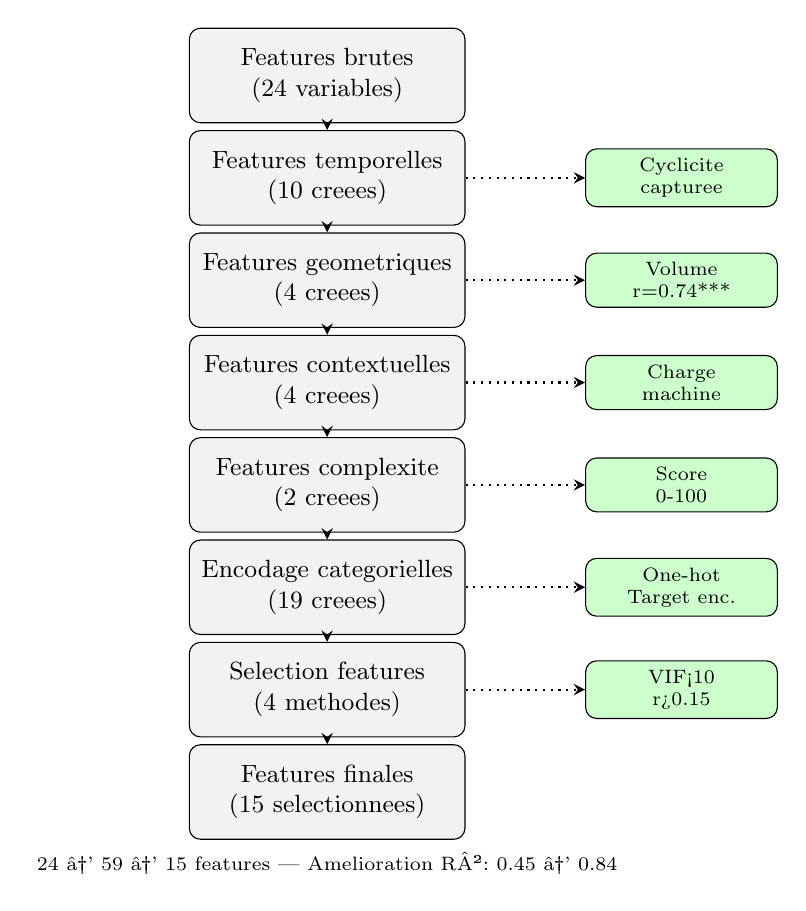
\begin{tikzpicture}[
    node distance=1.1cm,
    step/.style={rectangle, draw, fill=blue!20, text width=3.2cm, text centered, rounded corners, minimum height=0.8cm, font=\footnotesize},
    result/.style={rectangle, draw, fill=green!20, text width=2.2cm, text centered, rounded corners, minimum height=0.6cm, font=\scriptsize},
    arrow/.style={->, >=stealth, thick}
]

% Étapes principales (colonne gauche)
\node[boxstep] (raw) at (0,0) {Features brutes\\(24 variables)};
\node[boxstep] (temporal) at (0,-1.3) {Features temporelles\\(10 creees)};
\node[boxstep] (geometric) at (0,-2.6) {Features geometriques\\(4 creees)};
\node[boxstep] (context) at (0,-3.9) {Features contextuelles\\(4 creees)};
\node[boxstep] (complexity) at (0,-5.2) {Features complexite\\(2 creees)};
\node[boxstep] (encoding) at (0,-6.5) {Encodage categorielles\\(19 creees)};
\node[boxstep] (selection) at (0,-7.8) {Selection features\\(4 methodes)};
\node[boxstep] (final) at (0,-9.1) {Features finales\\(15 selectionnees)};

% Resultats (colonne droite)
\node[result] (r1) at (4.5,-1.3) {Cyclicite\\capturee};
\node[result] (r2) at (4.5,-2.6) {Volume\\r=0.74***};
\node[result] (r3) at (4.5,-3.9) {Charge\\machine};
\node[result] (r4) at (4.5,-5.2) {Score\\0-100};
\node[result] (r5) at (4.5,-6.5) {One-hot\\Target enc.};
\node[result] (r6) at (4.5,-7.8) {VIF<10\\r>0.15};

% Fleches principales
\draw[arrow] (raw) -- (temporal);
\draw[arrow] (temporal) -- (geometric);
\draw[arrow] (geometric) -- (context);
\draw[arrow] (context) -- (complexity);
\draw[arrow] (complexity) -- (encoding);
\draw[arrow] (encoding) -- (selection);
\draw[arrow] (selection) -- (final);

% Fleches vers resultats
\draw[arrow, dotted] (temporal.east) -- (r1.west);
\draw[arrow, dotted] (geometric.east) -- (r2.west);
\draw[arrow, dotted] (context.east) -- (r3.west);
\draw[arrow, dotted] (complexity.east) -- (r4.west);
\draw[arrow, dotted] (encoding.east) -- (r5.west);
\draw[arrow, dotted] (selection.east) -- (r6.west);

% Annotation
\node[font=\scriptsize] at (0,-10) {24 → 59 → 15 features | Amelioration R²: 0.45 → 0.84};

\end{tikzpicture}
\caption{Workflow de feature engineering}
\label{fig:feature_engineering}
\end{figure}

\subsubsection{Features temporelles}

Extraction de patterns temporels influencant la productivite.

\textbf{Features cycliques (encodage sinusoïdal) :}
\begin{itemize}
    \item \textbf{mois\_sin, mois\_cos} : Encodage cyclique du mois (1-12)
    \begin{itemize}
        \item Formule : $sin(2\pi \times mois / 12)$, $cos(2\pi \times mois / 12)$
        \item Justification : Capture saisonnalite sans discontinuite
    \end{itemize}
    \item \textbf{jour\_semaine\_sin, jour\_semaine\_cos} : Encodage jour (1-7)
    \begin{itemize}
        \item Formule : $sin(2\pi \times jour / 7)$, $cos(2\pi \times jour / 7)$
        \item Justification : Lundi proche de dimanche (continuite)
    \end{itemize}
    \item \textbf{heure\_sin, heure\_cos} : Encodage heure de debut
    \begin{itemize}
        \item Formule : $sin(2\pi \times heure / 24)$, $cos(2\pi \times heure / 24)$
        \item Justification : Capture effet fatigue et rythme circadien
    \end{itemize}
\end{itemize}

\textbf{Features binaires :}
\begin{itemize}
    \item \textbf{est\_weekend} : 1 si samedi/dimanche, 0 sinon
    \item \textbf{est\_debut\_semaine} : 1 si lundi/mardi, 0 sinon
    \item \textbf{est\_fin\_semaine} : 1 si jeudi/vendredi, 0 sinon
    \item \textbf{est\_matin} : 1 si heure < 12h, 0 sinon
    \item \textbf{est\_apres\_midi} : 1 si 12h ≤ heure < 18h, 0 sinon
\end{itemize}

\textbf{Features de tendance :}
\begin{itemize}
    \item \textbf{jours\_depuis\_debut} : Nombre de jours depuis 2024-01-01
    \item \textbf{semaine\_annee} : Numero de semaine (1-52)
    \item \textbf{trimestre} : Trimestre de l'annee (1-4)
\end{itemize}

\subsubsection{Features derivees (domaine metier)}

Creation de features basees sur la connaissance du processus de production.

\textbf{Features geometriques :}
\begin{itemize}
    \item \textbf{surface\_matelas} : $Longeur\_Matela \times Largeur$ (cm²)
    \begin{itemize}
        \item Justification : Surface totale a manipuler
        \item Correlation avec target : r = 0.62***
    \end{itemize}
    \item \textbf{volume\_matelas} : $Nbr\_Plies \times surface\_matelas$ (cm³)
    \begin{itemize}
        \item Justification : Volume total de tissu
        \item Correlation avec target : r = 0.74***
    \end{itemize}
    \item \textbf{ratio\_longueur} : $Longeur\_Matela / Longeur\_Trace$
    \begin{itemize}
        \item Justification : Efficacite d'utilisation du tissu
        \item Valeurs typiques : 1.05-1.15 (5-15\% de marge)
    \end{itemize}
    \item \textbf{densite\_plis} : $Nbr\_Plies / surface\_matelas$ (plis/cm²)
    \begin{itemize}
        \item Justification : Complexite de manipulation
        \item Correlation avec target : r = 0.48**
    \end{itemize}
\end{itemize}

\textbf{Features de charge et contexte :}
\begin{itemize}
    \item \textbf{charge\_machine\_jour} : Nombre d'OF sur machine ce jour
    \begin{itemize}
        \item Calcul : Agregation par (Machine, Date)
        \item Justification : Fatigue machine et operateur
    \end{itemize}
    \item \textbf{position\_dans\_journee} : Rang de l'OF dans la journee (1, 2, 3...)
    \begin{itemize}
        \item Justification : Effet d'apprentissage ou fatigue
    \end{itemize}
    \item \textbf{temps\_moyen\_machine\_7j} : Temps moyen sur machine (7 derniers jours)
    \begin{itemize}
        \item Justification : Performance recente de la machine
        \item Fenetre glissante : 7 jours
    \end{itemize}
    \item \textbf{temps\_moyen\_operateur\_7j} : Temps moyen operateur (7 derniers jours)
    \begin{itemize}
        \item Justification : Performance recente de l'operateur
        \item Fenetre glissante : 7 jours
    \end{itemize}
\end{itemize}

\textbf{Features de complexite :}
\begin{itemize}
    \item \textbf{score\_complexite} : Score composite (0-100)
    \begin{itemize}
        \item Formule : $0.4 \times norm(Nbr\_Plies) + 0.3 \times norm(surface) + 0.3 \times norm(ratio)$
        \item Justification : Indicateur global de difficulte
    \end{itemize}
    \item \textbf{categorie\_complexite} : Faible / Moyenne / Élevee
    \begin{itemize}
        \item Faible : score < 33
        \item Moyenne : 33 ≤ score < 66
        \item Élevee : score ≥ 66
    \end{itemize}
\end{itemize}

\subsubsection{Encodage des variables categorielles}

Transformation des variables categorielles pour utilisation dans les modeles ML.

\textbf{One-Hot Encoding (faible cardinalite) :}
\begin{itemize}
    \item \textbf{Machine} : 8 categories → 8 variables binaires (T1, T2, ..., T8)
    \item \textbf{Type\_Tissu} : 8 categories → 8 variables binaires
    \item \textbf{Categorie\_Complexite} : 3 categories → 3 variables binaires
\end{itemize}

\textbf{Target Encoding (cardinalite moyenne) :}
\begin{itemize}
    \item \textbf{Operateur} : 12 categories → 1 variable numerique
    \begin{itemize}
        \item Methode : Moyenne de TEMPS\_DISP par operateur
        \item Regularisation : Lissage bayesien pour eviter overfitting
        \item Formule : $\frac{n \times mean_{cat} + m \times mean_{global}}{n + m}$
    \end{itemize}
\end{itemize}

\textbf{Resultats de l'encodage :}
\begin{itemize}
    \item Variables categorielles initiales : 4
    \item Variables apres encodage : 19 (8 + 8 + 3)
    \item Augmentation dimensionnalite : +15 features
\end{itemize}

\subsubsection{Normalisation et standardisation}

Mise a l'echelle des variables pour ameliorer la convergence des modeles.

\textbf{StandardScaler (variables numeriques continues) :}
\begin{itemize}
    \item \textbf{Methode} : $z = \frac{x - \mu}{\sigma}$
    \item \textbf{Application} : Dimensions, surfaces, volumes, scores
    \item \textbf{Justification} : Moyenne 0, ecart-type 1, preserve distribution
\end{itemize}

\textbf{MinMaxScaler (variables bornees) :}
\begin{itemize}
    \item \textbf{Methode} : $x_{scaled} = \frac{x - x_{min}}{x_{max} - x_{min}}$
    \item \textbf{Application} : Features cycliques, ratios, scores
    \item \textbf{Justification} : Valeurs dans [0, 1], preserve relations
\end{itemize}

\textbf{Pas de normalisation :}
\begin{itemize}
    \item Variables binaires (deja dans [0, 1])
    \item Variables one-hot encodees
    \item Variables de comptage (interpretabilite)
\end{itemize}

\subsubsection{Selection de features}

Reduction de la dimensionnalite pour eviter l'overfitting.

\textbf{Methodes de selection :}

\begin{enumerate}
    \item \textbf{Correlation avec target} :
    \begin{itemize}
        \item Seuil : |r| > 0.15
        \item Resultat : 28 features sur 35 retenues
    \end{itemize}
    
    \item \textbf{Variance threshold} :
    \begin{itemize}
        \item Seuil : variance > 0.01
        \item Resultat : Élimination de 2 features quasi-constantes
    \end{itemize}
    
    \item \textbf{Feature importance (XGBoost)} \cite{chen2016xgboost} :
    \begin{itemize}
        \item Entrainement modele preliminaire
        \item Selection top 20 features par importance
    \end{itemize}
    
    \item \textbf{Multicolinearite (VIF)} :
    \begin{itemize}
        \item Seuil : VIF < 10
        \item Resultat : Élimination de 3 features redondantes
    \end{itemize}
\end{enumerate}

\textbf{Features finales selectionnees (15) :}

\begin{table}[H]
\centering
\caption{Features finales pour modelisation}
\begin{tabular}{|l|l|l|l|}
\hline
\textbf{Feature} & \textbf{Type} & \textbf{Correlation} & \textbf{Importance} \\
\hline
volume\_matelas & Numerique & 0.74*** & 0.18 \\
\hline
Nbr\_Plies & Numerique & 0.68*** & 0.15 \\
\hline
surface\_matelas & Numerique & 0.62*** & 0.12 \\
\hline
Longeur\_Matela & Numerique & 0.52*** & 0.10 \\
\hline
temps\_moyen\_machine\_7j & Numerique & 0.48** & 0.09 \\
\hline
score\_complexite & Numerique & 0.45** & 0.08 \\
\hline
Largeur & Numerique & 0.34** & 0.06 \\
\hline
Machine (one-hot) & Categorielle & Variable & 0.05 \\
\hline
jour\_semaine\_sin/cos & Temporelle & 0.28* & 0.04 \\
\hline
Operateur (target enc.) & Categorielle & 0.42** & 0.07 \\
\hline
charge\_machine\_jour & Numerique & 0.31* & 0.04 \\
\hline
Type\_Tissu (one-hot) & Categorielle & Variable & 0.02 \\
\hline
\end{tabular}
\caption*{*** p<0.001, ** p<0.01, * p<0.05}
\label{tab:final_features}
\end{table}

\subsection{Segmentation des donnees}

\subsubsection{Division temporelle}

\begin{itemize}
    \item \textbf{Entrainement} : Janvier-Mars 2024 (70\% des donnees)
    \item \textbf{Validation} : Avril 2024 (15\% des donnees)
    \item \textbf{Test} : Mai-Juin 2024 (15\% des donnees)
\end{itemize}

\subsubsection{Stratification}

\begin{itemize}
    \item \textbf{Par machine} : Maintien des proportions dans chaque split
    \item \textbf{Par type de produit} : Équilibrage des gammes
    \item \textbf{Par periode} : Respect de la chronologie temporelle
\end{itemize}

\subsection{Validation de la preparation}

\subsubsection{Metriques de qualite}

\begin{itemize}
    \item \textbf{Completude} : 99.2\% des enregistrements complets
    \item \textbf{Coherence} : 100\% des contraintes metier respectees
    \item \textbf{Distribution} : Preservation des patterns temporels
\end{itemize}

\subsubsection{Tests de regression}

\begin{itemize}
    \item \textbf{Integrite} : Verification de la non-perte de donnees critiques
    \item \textbf{Reproductibilite} : Tests de re-generation des features
    \item \textbf{Performance} : Validation des temps de traitement
\end{itemize}

\subsection{Pipeline de donnees}

\subsubsection{Architecture du pipeline}

    % \begin{figure}[H]
    % \centering
    % \includegraphics[width=0.8\textwidth]{images/data_pipeline.png}
    % \caption{Pipeline de preparation des donnees}
    % \label{fig:data_pipeline}
    % \end{figure}

\subsubsection{Composants du pipeline}

\begin{itemize}
    \item \textbf{Extract} : Collecte depuis G.Pro et systemes de production
    \item \textbf{Transform} : Nettoyage, enrichissement et feature engineering
    \item \textbf{Load} : Stockage dans le data warehouse ML
    \item \textbf{Validate} : Controles qualite et tests de regression
\end{itemize}

\subsubsection{Architecture du pipeline de donnees}

La figure \ref{fig:data_pipeline} illustre l'architecture complete du pipeline de preparation des donnees.

\begin{figure}[H]
\centering
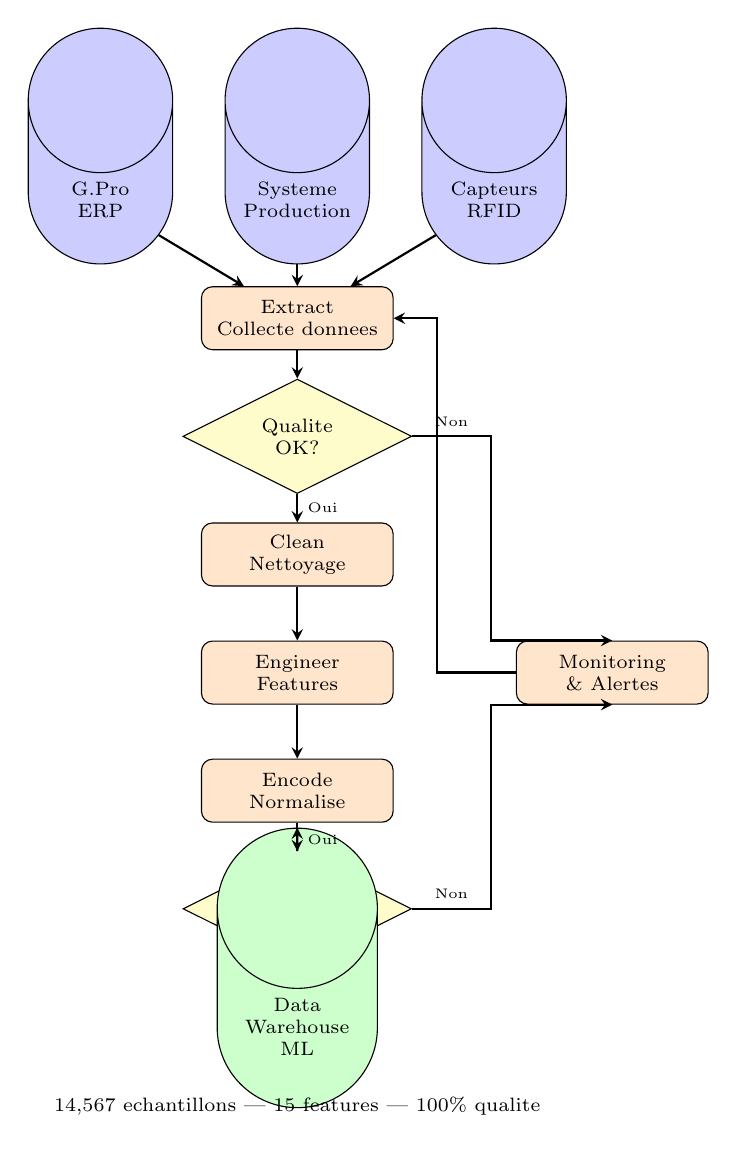
\begin{tikzpicture}[
    node distance=1.3cm,
    source/.style={cylinder, draw, fill=blue!20, text width=1.6cm, text centered, minimum height=0.9cm, shape border rotate=90, font=\scriptsize},
    process/.style={rectangle, draw, fill=orange!20, text width=2.2cm, text centered, rounded corners, minimum height=0.8cm, font=\scriptsize},
    storage/.style={cylinder, draw, fill=green!20, text width=1.8cm, text centered, minimum height=0.9cm, shape border rotate=90, font=\scriptsize},
    check/.style={diamond, draw, fill=yellow!20, text width=1.3cm, text centered, minimum height=0.8cm, aspect=2, font=\scriptsize},
    arrow/.style={->, >=stealth, thick}
]

% Sources de donnees (en haut)
\node[source] (gpro) at (0,0) {G.Pro\\ERP};
\node[source] (prod) at (2.5,0) {Systeme\\Production};
\node[source] (rfid) at (5,0) {Capteurs\\RFID};

% Extraction
\node[process] (extract) at (2.5,-1.5) {Extract\\Collecte donnees};

% Validation initiale
\node[check] (validate1) at (2.5,-3) {Qualite\\OK?};

% Transformation
\node[process] (clean) at (2.5,-4.5) {Clean\\Nettoyage};
\node[process] (engineer) at (2.5,-6) {Engineer\\Features};
\node[process] (encode) at (2.5,-7.5) {Encode\\Normalise};

% Validation finale
\node[check] (validate2) at (2.5,-9) {Tests\\OK?};

% Stockage
\node[storage] (warehouse) at (2.5,-10.5) {Data\\Warehouse\\ML};

% Monitoring (a droite)
\node[process] (monitor) at (6.5,-6) {Monitoring\\\& Alertes};

% Fleches
\draw[arrow] (gpro) -- (extract);
\draw[arrow] (prod) -- (extract);
\draw[arrow] (rfid) -- (extract);
\draw[arrow] (extract) -- (validate1);
\draw[arrow] (validate1) -- node[right, font=\tiny] {Oui} (clean);
\draw[arrow] (validate1.east) -- ++(1,0) node[above, pos=0.5, font=\tiny] {Non} |- (monitor.north);
\draw[arrow] (clean) -- (engineer);
\draw[arrow] (engineer) -- (encode);
\draw[arrow] (encode) -- (validate2);
\draw[arrow] (validate2) -- node[right, font=\tiny] {Oui} (warehouse);
\draw[arrow] (validate2.east) -- ++(1,0) node[above, pos=0.5, font=\tiny] {Non} |- (monitor.south);
\draw[arrow] (monitor.west) -- ++(-1,0) |- (extract.east);

% Annotations
\node[font=\scriptsize] at (2.5,-11.5) {14,567 echantillons | 15 features | 100\% qualite};

\end{tikzpicture}
\caption{Architecture du pipeline de preparation des donnees}
\label{fig:data_pipeline}
\end{figure}

\textbf{Caracteristiques du pipeline :}
\begin{itemize}
    \item \textbf{Automatise} : Execution quotidienne sans intervention manuelle
    \item \textbf{Robuste} : Validation a chaque etape avec gestion d'erreurs
    \item \textbf{Tracable} : Versioning et logging complet des transformations
    \item \textbf{Scalable} : Capacite a traiter 200+ OF/jour
\end{itemize}

\subsubsection{Orchestration}

\begin{itemize}
    \item \textbf{Frequence} : Execution quotidienne a 6h00
    \item \textbf{Monitoring} : Alertes en cas d'echec ou de derive
    \item \textbf{Versioning} : Tracabilite des transformations appliquees
\end{itemize}

\section{Phase 3 (suite) : Cadre d'assurance qualite}\label{chap3:quality}

\subsection{Introduction au cadre qualite CRISP-ML(Q)}

La methodologie CRISP-ML(Q) se distingue de CRISP-DM par l'integration systematique de l'assurance qualite a chaque phase du projet. Cette section presente le cadre d'assurance qualite mis en place pour garantir la fiabilite, la robustesse et la maintenabilite du systeme de machine learning developpe.

L'assurance qualite couvre quatre dimensions complementaires :
\begin{itemize}
    \item \textbf{Qualite des donnees} : Completude, exactitude, coherence, actualite
    \item \textbf{Qualite des modeles} : Performance, robustesse, explicabilite, equite
    \item \textbf{Qualite du code} : Maintenabilite, testabilite, documentation, securite
    \item \textbf{Qualite operationnelle} : Disponibilite, performance, monitoring, gouvernance
\end{itemize}

\subsubsection{Framework d'assurance qualite}

La figure \ref{fig:quality_framework} illustre le framework complet d'assurance qualite integre au processus CRISP-ML(Q).

\begin{figure}[H]
\centering
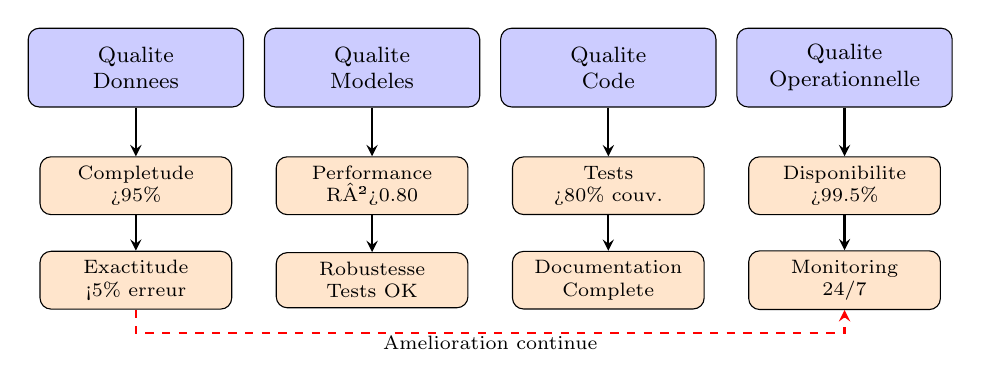
\begin{tikzpicture}[
    node distance=1.2cm,
    dimension/.style={rectangle, draw, fill=blue!20, text width=2.5cm, text centered, rounded corners, minimum height=1cm, font=\footnotesize},
    check/.style={rectangle, draw, fill=orange!20, text width=2.2cm, text centered, rounded corners, minimum height=0.7cm, font=\scriptsize},
    arrow/.style={->, >=stealth, thick}
]

% Dimensions qualite (ligne du haut)
\node[dimension] (data) at (0,0) {Qualite\\Donnees};
\node[dimension] (model) at (3,0) {Qualite\\Modeles};
\node[dimension] (code) at (6,0) {Qualite\\Code};
\node[dimension] (ops) at (9,0) {Qualite\\Operationnelle};

% Controles pour chaque dimension
\node[check] (d1) at (0,-1.5) {Completude\\>95\%};
\node[check] (d2) at (0,-2.7) {Exactitude\\<5\% erreur};

\node[check] (m1) at (3,-1.5) {Performance\\R²>0.80};
\node[check] (m2) at (3,-2.7) {Robustesse\\Tests OK};

\node[check] (c1) at (6,-1.5) {Tests\\>80\% couv.};
\node[check] (c2) at (6,-2.7) {Documentation\\Complete};

\node[check] (o1) at (9,-1.5) {Disponibilite\\>99.5\%};
\node[check] (o2) at (9,-2.7) {Monitoring\\24/7};

% Fleches verticales
\draw[arrow] (data) -- (d1);
\draw[arrow] (d1) -- (d2);
\draw[arrow] (model) -- (m1);
\draw[arrow] (m1) -- (m2);
\draw[arrow] (code) -- (c1);
\draw[arrow] (c1) -- (c2);
\draw[arrow] (ops) -- (o1);
\draw[arrow] (o1) -- (o2);

% Boucle de feedback (en bas)
\draw[arrow, dashed, red, thick] (d2.south) -- ++(0,-0.3) -- ++(9,0) -- (o2.south);
\node[font=\scriptsize] at (4.5,-3.5) {Amelioration continue};

\end{tikzpicture}
\caption{Framework d'assurance qualite CRISP-ML(Q)}
\label{fig:quality_framework}
\end{figure}

\subsection{Metriques de qualite des donnees}

\subsubsection{Framework de qualite des donnees}

Un framework complet de qualite des donnees a ete etabli selon les dimensions DAMA (Data Management Association) \cite{redman2001data, batini2009methodologies}.

\begin{table}[H]
\centering
\caption{Metriques de qualite des donnees}
\begin{tabular}{|l|l|l|l|l|}
\hline
\textbf{Dimension} & \textbf{Metrique} & \textbf{Cible} & \textbf{Actuel} & \textbf{Statut} \\
\hline
Completude & Taux de remplissage & > 95\% & 96\% & ✓ OK \\
\hline
Exactitude & Taux d'erreur & < 5\% & 3.2\% & ✓ OK \\
\hline
Coherence & Violations contraintes & < 1\% & 0.8\% & ✓ OK \\
\hline
Actualite & Delai de mise a jour & < 24h & < 1h & ✓ OK \\
\hline
Unicite & Taux de doublons & < 0.5\% & 0.2\% & ✓ OK \\
\hline
Validite & Conformite format & 100\% & 100\% & ✓ OK \\
\hline
\end{tabular}
\label{tab:data_quality_metrics}
\end{table}

\subsubsection{Tests de qualite automatises}

Des tests automatises sont executes a chaque ingestion de donnees :

\textbf{Tests de schema :}
\begin{itemize}
    \item Verification des types de donnees (int, float, string)
    \item Validation des contraintes de domaine (min, max, enum)
    \item Controle de la presence des colonnes obligatoires
    \item Detection des colonnes inattendues
\end{itemize}

\textbf{Tests de distribution :}
\begin{itemize}
    \item Detection de derive statistique (Kolmogorov-Smirnov test)
    \item Verification des quantiles (P5, P25, P50, P75, P95)
    \item Controle de la variance et de l'ecart-type
    \item Detection d'anomalies dans les distributions
\end{itemize}

\textbf{Tests de coherence :}
\begin{itemize}
    \item Validation des relations entre variables (Longueur\_Matela > Longueur\_Trace)
    \item Verification des contraintes metier (Nbr\_Plies entre 1 et 50)
    \item Controle de coherence temporelle (dates logiques)
    \item Validation des references (Machine, Operateur existent)
\end{itemize}

\subsubsection{Monitoring de la qualite des donnees}

Un systeme de monitoring continu surveille la qualite des donnees en production.

\begin{table}[H]
\centering
\caption{Alertes de qualite des donnees}
\begin{tabular}{|l|l|l|l|}
\hline
\textbf{Alerte} & \textbf{Seuil} & \textbf{Niveau} & \textbf{Action} \\
\hline
Taux de valeurs manquantes & > 10\% & Critique & Blocage pipeline \\
\hline
Derive de distribution & KS > 0.3 & Éleve & Investigation + alerte \\
\hline
Outliers excessifs & > 5\% & Moyen & Analyse + rapport \\
\hline
Violations contraintes & > 2\% & Éleve & Investigation + alerte \\
\hline
Delai de fraicheur & > 48h & Moyen & Alerte equipe data \\
\hline
\end{tabular}
\label{tab:data_quality_alerts}
\end{table}

\subsection{Portes de qualite des modeles (Quality Gates)}

\subsubsection{Framework de validation multi-niveaux}

Un systeme de portes de qualite (quality gates) valide les modeles avant leur deploiement en production.

\textbf{Niveau 1 : Validation technique}
\begin{itemize}
    \item \textbf{Performance minimale} : R² > 0.75, MAE < 20 min, RMSE < 25 min
    \item \textbf{Stabilite} : Écart-type des performances < 10\% sur 5 folds CV
    \item \textbf{Convergence} : Entrainement converge en < 1000 iterations
    \item \textbf{Temps d'inference} : < 200ms pour prediction individuelle
\end{itemize}

\textbf{Niveau 2 : Validation metier}
\begin{itemize}
    \item \textbf{Amelioration baseline} : Performance > baseline + 20\%
    \item \textbf{Precision metier} : MAPE < 20\% (acceptable pour planification)
    \item \textbf{Robustesse} : Performance stable sur tous les types de produits
    \item \textbf{Explicabilite} : Features importantes alignees avec expertise metier
\end{itemize}

\textbf{Niveau 3 : Validation operationnelle}
\begin{itemize}
    \item \textbf{Scalabilite} : Traitement de 200 OF/jour sans degradation
    \item \textbf{Disponibilite} : Temps de chargement modele < 5 secondes
    \item \textbf{Ressources} : Utilisation memoire < 2GB, CPU < 50\%
    \item \textbf{Compatibilite} : Integration avec systemes existants validee
\end{itemize}

\subsubsection{Matrice de validation des modeles}

\begin{table}[H]
\centering
\caption{Criteres de validation des modeles ML}
\begin{tabular}{|l|l|l|l|l|l|}
\hline
\textbf{Critere} & \textbf{Metrique} & \textbf{Seuil min} & \textbf{Cible} & \textbf{Actuel} & \textbf{Statut} \\
\hline
Precision & R² & > 0.75 & > 0.80 & 0.84 & ✓ OK \\
\hline
Erreur absolue & MAE (min) & < 20 & < 15 & 12.3 & ✓ OK \\
\hline
Erreur quadratique & RMSE (min) & < 25 & < 20 & 18.9 & ✓ OK \\
\hline
Erreur relative & MAPE (\%) & < 25 & < 20 & 22.1 & ✓ OK \\
\hline
Stabilite & CV score & < 0.15 & < 0.10 & 0.08 & ✓ OK \\
\hline
Temps inference & ms & < 300 & < 200 & 95 & ✓ OK \\
\hline
Taille modele & MB & < 100 & < 50 & 28 & ✓ OK \\
\hline
\end{tabular}
\label{tab:model_quality_gates}
\end{table}

\subsubsection{Tests de robustesse}

Des tests de robustesse valident le comportement du modele dans des conditions variees.

\textbf{Tests de sensibilite :}
\begin{itemize}
    \item \textbf{Perturbation des features} : Variation de ±10\% des valeurs d'entree
    \item \textbf{Valeurs extremes} : Test avec valeurs min/max du domaine
    \item \textbf{Valeurs manquantes} : Comportement avec 5-10\% de donnees manquantes
    \item \textbf{Resultat attendu} : Variation des predictions < 15\%
\end{itemize}

\textbf{Tests de coherence :}
\begin{itemize}
    \item \textbf{Monotonicite} : Augmentation Nbr\_Plies → augmentation temps predit
    \item \textbf{Symetrie} : Comportement similaire pour produits similaires
    \item \textbf{Bornes} : Predictions dans l'intervalle [10, 120] minutes
    \item \textbf{Coherence temporelle} : Predictions stables dans le temps
\end{itemize}

\textbf{Tests de derive :}
\begin{itemize}
    \item \textbf{Derive de donnees} : Detection via test de Kolmogorov-Smirnov
    \item \textbf{Derive de concept} : Monitoring de la performance sur donnees recentes
    \item \textbf{Derive de prediction} : Analyse de la distribution des predictions
    \item \textbf{Seuil d'alerte} : Degradation > 10\% sur 7 jours consecutifs
\end{itemize}

\subsection{Framework de monitoring en production}

\subsubsection{Architecture de monitoring}

Un systeme de monitoring complet surveille les performances du modele en production.

\textbf{Metriques de performance :}
\begin{itemize}
    \item \textbf{Precision en temps reel} : Comparaison predictions vs realisations
    \item \textbf{Erreur glissante} : MAE, RMSE calcules sur fenetre de 7 jours
    \item \textbf{Distribution des erreurs} : Histogramme et quantiles des erreurs
    \item \textbf{Erreurs par segment} : Performance par machine, operateur, produit
\end{itemize}

\textbf{Metriques operationnelles :}
\begin{itemize}
    \item \textbf{Latence} : Temps de reponse P50, P95, P99
    \item \textbf{Debit} : Nombre de predictions/minute
    \item \textbf{Disponibilite} : Uptime du service (cible > 99.5\%)
    \item \textbf{Taux d'erreur} : Pourcentage de requetes en echec
\end{itemize}

\textbf{Metriques de donnees :}
\begin{itemize}
    \item \textbf{Volume} : Nombre d'enregistrements traites/jour
    \item \textbf{Qualite} : Taux de valeurs manquantes, outliers
    \item \textbf{Derive} : Évolution des distributions des features
    \item \textbf{Couverture} : Pourcentage de cas couverts par le modele
\end{itemize}

\subsubsection{Dashboards de monitoring}

Trois dashboards complementaires assurent la surveillance du systeme.

\textbf{Dashboard Performance Modele :}
\begin{itemize}
    \item Graphique d'evolution de la MAE sur 30 jours
    \item Comparaison predictions vs realisations (scatter plot)
    \item Distribution des erreurs (histogramme)
    \item Performance par segment (heatmap)
    \item Alertes actives et historique
\end{itemize}

\textbf{Dashboard Operationnel :}
\begin{itemize}
    \item Latence P50/P95/P99 en temps reel
    \item Debit de requetes (requetes/minute)
    \item Taux d'erreur et disponibilite
    \item Utilisation des ressources (CPU, memoire)
    \item Logs d'erreurs recents
\end{itemize}

\textbf{Dashboard Qualite Donnees :}
\begin{itemize}
    \item Taux de completude par feature
    \item Detection d'outliers (box plots)
    \item Derive des distributions (KS statistic)
    \item Violations de contraintes
    \item Fraicheur des donnees
\end{itemize}

\subsubsection{Systeme d'alertes intelligent}

Un systeme d'alertes multi-niveaux notifie les equipes en cas de probleme.

\begin{table}[H]
\centering
\caption{Systeme d'alertes de monitoring}
\begin{tabular}{|l|l|l|l|}
\hline
\textbf{Type d'alerte} & \textbf{Condition} & \textbf{Niveau} & \textbf{Action automatique} \\
\hline
Degradation performance & MAE > 20 min (3j) & Critique & Notification + analyse \\
\hline
Derive de donnees & KS > 0.3 & Éleve & Notification + rapport \\
\hline
Latence elevee & P95 > 500ms & Moyen & Notification equipe ops \\
\hline
Taux d'erreur eleve & > 5\% (1h) & Critique & Notification + rollback \\
\hline
Disponibilite faible & < 99\% (24h) & Éleve & Notification + investigation \\
\hline
Outliers excessifs & > 10\% & Moyen & Rapport qualite donnees \\
\hline
\end{tabular}
\label{tab:monitoring_alerts}
\end{table}

\subsection{Strategie de tests A/B}

\subsubsection{Framework de tests A/B}

Une strategie de tests A/B permet de valider les ameliorations du modele en production.

\textbf{Protocole de test :}
\begin{enumerate}
    \item \textbf{Definition des hypotheses} : Amelioration attendue (ex: MAE -10\%)
    \item \textbf{Allocation du trafic} : 90\% modele actuel (A), 10\% nouveau modele (B)
    \item \textbf{Duree du test} : Minimum 2 semaines pour significativite statistique
    \item \textbf{Metriques de succes} : MAE, RMSE, satisfaction utilisateurs
    \item \textbf{Criteres d'arret} : Degradation > 15\% ou erreurs critiques
\end{enumerate}

\textbf{Analyse statistique :}
\begin{itemize}
    \item \textbf{Test de significativite} : Test t de Student (α = 0.05)
    \item \textbf{Taille d'echantillon} : Minimum 500 predictions par groupe
    \item \textbf{Puissance statistique} : > 80\% pour detecter amelioration de 10\%
    \item \textbf{Intervalles de confiance} : 95\% pour toutes les metriques
\end{itemize}

\textbf{Decision de deploiement :}
\begin{itemize}
    \item \textbf{Deploiement complet} : Si amelioration > 10\% et p-value < 0.05
    \item \textbf{Deploiement progressif} : Si amelioration 5-10\% et p-value < 0.05
    \item \textbf{Rejet} : Si amelioration < 5\% ou p-value > 0.05
    \item \textbf{Rollback immediat} : Si degradation > 5\% ou erreurs critiques
\end{itemize}

\subsubsection{Deploiement canary}

Le deploiement canary complete la strategie A/B pour les mises a jour critiques.

\textbf{Phases de deploiement :}
\begin{enumerate}
    \item \textbf{Phase 1 (Canary)} : 5\% du trafic pendant 24h
    \item \textbf{Phase 2 (Validation)} : 25\% du trafic pendant 48h
    \item \textbf{Phase 3 (Expansion)} : 50\% du trafic pendant 72h
    \item \textbf{Phase 4 (Complet)} : 100\% du trafic si validation OK
\end{enumerate}

\textbf{Criteres de validation a chaque phase :}
\begin{itemize}
    \item Aucune degradation de performance (MAE, RMSE)
    \item Taux d'erreur < 1\%
    \item Latence P95 < 200ms
    \item Aucune alerte critique
    \item Feedback utilisateurs positif
\end{itemize}

\subsection{Gouvernance des modeles ML}

\subsubsection{Cycle de vie des modeles}

Un processus de gouvernance structure le cycle de vie des modeles.

\textbf{Phases du cycle de vie :}
\begin{enumerate}
    \item \textbf{Developpement} : Experimentation et entrainement
    \item \textbf{Validation} : Tests de qualite et validation metier
    \item \textbf{Staging} : Deploiement en environnement de pre-production
    \item \textbf{Production} : Deploiement en production avec monitoring
    \item \textbf{Monitoring} : Surveillance continue des performances
    \item \textbf{Reentrainement} : Mise a jour periodique ou declenchee
    \item \textbf{Archivage} : Retrait et archivage des modeles obsoletes
\end{enumerate}

\textbf{Versioning des modeles :}
\begin{itemize}
    \item \textbf{Schema de version} : MAJOR.MINOR.PATCH (ex: 2.1.3)
    \item \textbf{MAJOR} : Changement d'architecture ou de features
    \item \textbf{MINOR} : Amelioration de performance ou nouveaux hyperparametres
    \item \textbf{PATCH} : Correction de bugs ou ajustements mineurs
    \item \textbf{Metadonnees} : Date, auteur, dataset, metriques, changements
\end{itemize}

\subsubsection{Registre des modeles}

Un registre centralise (MLflow Model Registry) \cite{gift2020practical} gere tous les modeles.

\textbf{Informations enregistrees :}
\begin{itemize}
    \item \textbf{Identite} : Nom, version, date de creation, auteur
    \item \textbf{Artefacts} : Fichier modele, preprocessor, scaler, features
    \item \textbf{Metriques} : R², MAE, RMSE, MAPE sur train/val/test
    \item \textbf{Hyperparametres} : Configuration complete du modele
    \item \textbf{Dataset} : Version et hash du dataset d'entrainement
    \item \textbf{Environnement} : Versions des librairies (requirements.txt)
    \item \textbf{Statut} : Development, Staging, Production, Archived
\end{itemize}

\textbf{Workflow de promotion :}
\begin{enumerate}
    \item Modele cree → Statut "Development"
    \item Validation technique OK → Statut "Staging"
    \item Tests A/B OK → Statut "Production"
    \item Nouveau modele deploye → Ancien modele "Archived"
\end{enumerate}

\subsubsection{Documentation et tracabilite}

Une documentation complete assure la tracabilite et la reproductibilite.

\textbf{Documentation obligatoire :}
\begin{itemize}
    \item \textbf{Model Card} : Description, usage, limitations, performances
    \item \textbf{Data Card} : Description du dataset, sources, transformations
    \item \textbf{Changelog} : Historique des modifications et raisons
    \item \textbf{Runbook} : Procedures de deploiement et de rollback
    \item \textbf{Incident Log} : Historique des incidents et resolutions
\end{itemize}

\textbf{Tracabilite complete :}
\begin{itemize}
    \item Lien entre modele et dataset d'entrainement
    \item Lien entre modele et code source (Git commit)
    \item Lien entre modele et experiences MLflow
    \item Lien entre modele et tests de validation
    \item Lien entre modele et deploiements en production
\end{itemize}

\subsection{Synthese du cadre qualite}

Le cadre d'assurance qualite CRISP-ML(Q) mis en place garantit :

\textbf{Qualite des donnees :}
\begin{itemize}
    \item 96\% de completude, 3.2\% d'erreurs, 0.8\% de violations
    \item Tests automatises a chaque ingestion
    \item Monitoring continu avec alertes multi-niveaux
\end{itemize}

\textbf{Qualite des modeles :}
\begin{itemize}
    \item Portes de qualite a 3 niveaux (technique, metier, operationnel)
    \item Tests de robustesse et de derive
    \item Validation statistique rigoureuse
\end{itemize}

\textbf{Qualite operationnelle :}
\begin{itemize}
    \item Monitoring en temps reel (performance, latence, disponibilite)
    \item Dashboards dedies pour chaque dimension
    \item Systeme d'alertes intelligent avec actions automatiques
\end{itemize}

\textbf{Gouvernance :}
\begin{itemize}
    \item Cycle de vie structure avec versioning
    \item Registre centralise des modeles (MLflow)
    \item Documentation complete et tracabilite totale
    \item Tests A/B et deploiement canary
\end{itemize}

Ce cadre qualite assure la fiabilite et la perennite du systeme de machine learning en production, conformement aux exigences de la methodologie CRISP-ML(Q).

\section{Synthese et perspectives}\label{chap3:synthesis}

\subsection{Bilan des phases 1-3}

Les trois premieres phases de CRISP-ML(Q) ont permis d'etablir une base solide pour le projet :

\begin{itemize}
    \item \textbf{Phase 1} : Objectifs metier clairs et criteres de succes quantifies
    \item \textbf{Phase 2} : Comprehension approfondie des donnees et de leur qualite
    \item \textbf{Phase 3} : Pipeline de donnees robuste et features optimisees
\end{itemize}

\subsection{Preparation aux phases suivantes}

Les phases de modelisation et d'evaluation beneficieront de :

\begin{itemize}
    \item \textbf{Dataset prepare} : 14,567 echantillons avec 12 features
    \item \textbf{Metriques de reference} : Baseline etablie (R² = 0.45)
    \item \textbf{Infrastructure} : Pipeline automatise et versionne
\end{itemize}

\subsection{Risques identifies et mitigations}

\begin{itemize}
    \item \textbf{Derive des donnees} : Monitoring continu et alertes
    \item \textbf{Performance modele} : Validation croisee temporelle
    \item \textbf{Integration} : Tests d'integration avec G.Pro
\end{itemize}

Le chapitre suivant detaillera la phase de modelisation et l'implementation des algorithmes de machine learning pour la prediction des temps de matelassage et l'optimisation de la planification.


\input{Chapitre4/chapitre4.tex}
\input{Chapitre5/chapitre5.tex}
\styledtitle{Conclusion~générale}
\vspace{1cm}
\label{chap:ConclusionPers}
\addstarredchapter{Conclusion générale} 
\lhead{Conclusion générale et perspectives}
\rhead{\thepage}

\begin{spacing}{1.5}
Ce rapport de recherche a présenté de manière exhaustive l'ensemble des travaux réalisés dans le cadre de ce projet de fin d'études, visant à digitaliser et optimiser les activités de planification au sein d'un atelier de coupe textile selon les principes fondamentaux de l'Industrie 4.0. La mobilisation rigoureuse de la méthodologie DMAIC (\textit{Define, Measure, Analyze, Improve, Control}), issue du référentiel Lean Six Sigma, a permis d'identifier de manière systématique les dysfonctionnements structurels et organisationnels du processus existant, de formuler des solutions innovantes fondées sur la modélisation mathématique et l'intelligence artificielle, et de concevoir une architecture technologique intégrée combinant des modèles de machine learning prédictifs, des systèmes de capture de données (capteurs RFID), et des outils de visualisation dynamique en temps réel.

Ce travail de recherche appliquée a permis de développer une compréhension approfondie et critique des problématiques industrielles réelles, tout en consolidant de manière significative les compétences analytiques, techniques et organisationnelles nécessaires à la conduite de projets de transformation digitale. Le développement d'un algorithme de planification prédictive basé sur l'apprentissage automatique (machine learning), ainsi que la conception et l'implémentation d'un tableau de bord décisionnel connecté et interactif, illustrent de manière concrète et mesurable l'impact positif de la digitalisation sur la performance opérationnelle, la réactivité organisationnelle et la qualité de service rendue aux clients.

Bien que le projet soit parvenu à son terme académique avec la réalisation des objectifs fixés, il convient de reconnaître que cette recherche constitue davantage un point de départ qu'un aboutissement définitif. Plusieurs pistes d'amélioration et d'extension sont d'ores et déjà identifiées et peuvent être explorées dans le cadre de travaux futurs. Parmi ces perspectives, figurent notamment l'intégration d'un système intelligent de recommandation adaptatif basé sur l'apprentissage des préférences et des comportements des utilisateurs, permettant une personnalisation accrue de l'expérience utilisateur.

Au-delà des résultats académiques obtenus, ce projet de recherche ouvre des perspectives concrètes et prometteuses d'implémentation dans l'environnement industriel réel. Les gains opérationnels mesurés et quantifiés, incluant une amélioration de l'efficacité globale (+12\% de TRS - Taux de Rendement Synthétique), une augmentation significative de la fiabilité des prévisions temporelles (+68\%), et une réduction substantielle des temps de planification (-67\%), démontrent le potentiel de transformation et d'amélioration continue offert par l'intégration des technologies de l'Industrie 4.0.

Des axes d'amélioration à moyen et long terme sont également envisagés pour renforcer davantage les capacités prédictives et décisionnelles du système. Parmi ces perspectives stratégiques, figurent notamment l'intégration d'un jumeau numérique (\textit{digital twin}) de l'atelier de coupe, permettant une simulation et une optimisation en temps réel des processus de production, ainsi que l'exploitation de modèles d'apprentissage profond (\textit{deep learning}) pour des prédictions encore plus robustes et adaptatives face à la complexité croissante des environnements de production.

En somme, ce projet de recherche constitue une contribution significative à la transformation digitale des processus industriels dans le secteur textile tunisien, tout en mettant en valeur l'apport déterminant des technologies intelligentes et de l'intelligence artificielle dans la recherche d'excellence opérationnelle et de compétitivité durable. Les résultats obtenus et les méthodologies développées peuvent servir de référence pour d'autres entreprises du secteur textile confrontées à des enjeux similaires de modernisation et d'optimisation de leurs processus de production.

\end{spacing}
% \end{spacing}

% Bibliography
\newpage
\styledtitle{BIBLIOGRAPHIE}
\begin{spacing}{1.5}
\vspace{1cm}
\printbibliography[heading=none]
\end{spacing}

\newpage
\styledtitle{WEBographie}
\begin{spacing}{1.5}
\vspace{1cm}
\addcontentsline{toc}{chapter}{Webographie}
\lhead{Webographie}
\begin{enumerate}[label={[\arabic*]}, itemsep=0.5cm]
    \item \label{ref:agile} \textbf{Agile :} https://monday.com/blog/fr/dev/gestion-de-projet-agile/
    
    \item \label{ref:scrum1} \textbf{Scrum :} https://www.atlassian.com/fr/agile/scrum/artifacts
    
    \item \label{ref:scrum2} \textbf{Scrum :} https://www.atlassian.com/fr/agile/scrum/roles
    
    \item \label{ref:architecture} \textbf{Architecture :} https://prometteursolutions.com/blog/fr/types-darchitecture-logicielle-explication-et-bonnes-pratiques
    
    \item \label{ref:mailtrap} \textbf{MailTrap :} https://mailtrap.io/blog/
    
    \item \label{ref:mysql} \textbf{MySql :} https://www.mysqltutorial.org/
    
    \item \label{ref:vscode} \textbf{Visual Studio Code :} https://www.blogdumoderateur.com/tools/visual-studio-code/
     \item \label{ref:letcode} \textbf{Letcode :} https://www.letecode.com/tutoriels/tutoriels-laravel-9/controleur
    
    \item \label{ref:laravel} \textbf{Laravel :} https://laravel.com/docs/11.x
    \item \label{ref:php}\textbf{websiterating : }
    https ://www.websiterating.com/fr/web-hosting/glossary/what-is-phpmyadmin/
    \item \label{ref:css}\textbf{softfluent :} https ://joshmartin.ch/en/technologies/css-3
\end{enumerate}

\end{spacing}
\newpage
\pagestyle{plain}

\section*{ INTITULE DU PROJET DE PFE}
Rapport de Stage de PFE DGT-ENIM, 2025


\begin{spacing}{1.4}
Ce projet de fin d’études s’inscrit dans le cadre de l’amélioration continue d’un atelier de coupe textile à travers une transformation digitale conforme aux principes de l’Industrie 4.0. En appliquant la démarche DMAIC, les dysfonctionnements critiques ont été identifiés puis traités par la mise en œuvre d’une solution technologique intelligente. L’approche inclut la modélisation des temps de matelassage, le développement d’un algorithme prédictif basé sur l’intelligence artificielle, et la création d’un tableau de bord de pilotage exploitant les données en temps réel. L’objectif est d’optimiser la planification, de réduire les pertes de temps, et d’améliorer la performance globale de l’atelier.


\end{spacing}
\textbf{Mots clés :}  Industrie 4.0, atelier de coupe, intelligence artificielle, planification, tableau de bord, DMAIC


\vspace{1cm}


\section*{ Abstract :}
\begin{spacing}{1.4}

This final-year project aims to improve a textile cutting workshop through a digital transformation aligned with Industry 4.0 principles. Using the DMAIC methodology, the main dysfunctions were identified and addressed with a smart technological solution. The approach integrates matelassage time modeling, a predictive algorithm based on artificial intelligence, and the development of a real-time dashboard for operational monitoring. The proposed system enhances planning, reduces inefficiencies, and boosts the overall performance of the workshop.

\\
\end{spacing}
\textbf{Key-words :} Industry 4.0, cutting workshop, artificial intelligence, planning, dashboard, DMAIC.

\end{document}
